\chapter{\java{} Applications on SGX}
\label{chap:civet}


\newcommand{\sysname}{Civet}
\newcommand{\jvm}{JVM}
\newcommand{\jvmname}{OpenJDK 7}
\newcommand{\staticphase}{design-time}
\newcommand{\statictool}{Shredder}
\newcommand{\dynamicphase}{execution-time}
%\newcommand{\dynamicframework}{Escalator}
\newcommand{\dynamicframework}{Connector}
\newcommand{\tcbsize}{trusted code size}


\makeatletter
\newcommand{\Capitalize}[1]{%
	\edef\@tempa{\expandafter\@gobble\string#1}%
	\edef\@tempb{\expandafter\@car\@tempa\@nil}%
	\edef\@tempa{\expandafter\@cdr\@tempa\@nil}%
	\uppercase\expandafter{\expandafter\def\expandafter\@tempb\expandafter{\@tempb}}%
	\@namedef{\@tempb\@tempa}{\expandafter\MakeUppercase\expandafter{#1}}}
\makeatother

\Capitalize{\dynamicphase}
\Capitalize{\staticphase}


\makeatletter
\def\input@path{{civet/}}
\makeatother
\graphicspath{{civet/figures/}}

\begin{abstract}

\intel{} \sgx{} hardware enables
applications to protect themselves from potentially-malicious
OSes or hypervisors.  
In cloud computing and other systems, many users and applications
could benefit from SGX. % protections.
Unfortunately, current applications will not work out-of-the-box on SGX.
Although previous work has shown that %, in principle,
a library OS can execute unmodified 
applications on SGX, a belief has developed that 
a library OS will be ruinous for performance and TCB size,
making 
application code modification
an implicit prerequisite to adopting SGX.

%A protected context is called an {\em enclave} include encrypting 


%isolates a program in an encrypted context, 
%called an {\em enclave},
%protecting it against malicious system components (e.g., rootkits),
%or hardware-level attacks (e.g., cold-boot attacks).
%\fixmedp{can we say something more precise?}
%\fixme{is this okay?}
% attacks from a compromised operating system (OS),
% hypervisor, or other sytem software.
%%to resist attacks from 
%%provide a tamper-resistant, isolated execution
%%environment for application code---a promising building block for secure systems.
%%has rapidly gained the attention of developer and research communities.
%Despite the fast-growing interest in \sgx{},
%%Despite a surge of research and development interest in \sgx{},
%adopting the hardware in existing applications has been far from efficient,
%due to the porting effort for overcoming the limitations of legacy frameworks.
%%% Current approaches to legacy application suuport on \sgx{}
%%% requires either modifying the binaries (SCONE, Panoply),
%%% or packaging all binaries into an encrypted archive to be provisioned from a remote server (Haven).
%%% \fixmedp{is this right?  What about Haven?}\fixme{Try to be clear}
%%% These requirements make adopting \sgx{} unstraightforward to unprofessional users.
%%% Moreover, COTS (commercial off-the-shelf) applications cannot be directly
%%% isolated by \sgx{} using the current approaches,
%%% due to difficulty of attesting off-the-shelf binaries
%%% and supporting the system ABI.
%%% For close-source applications or applications that requires modification
%%% to be ported to \sgx{},
%%% users need a framework to accelerate the porting process without the intervention of application developers.
%%% \fixme{is this better?}

%which make \sgx{} harder to adopt, if not impossible
%for closed-source applications without developer support.
%\fixmedp{I would rephrase these as problems, rather than benefits, but I don't understand these points yet:
%(2) reducing (re)deployment cost at upgrades.
%(3) isolating an application at emergency, with the measurement preserved for auditing.
%}

%As existing OS support for \sgx{} requires custom-making applications,
%Not only does Graphene simplify the effort to port an application
%to \sgx{}, but it also introduces benefits including:
%The COTS support not only minimizes the porting effort of an application to merely configuration,
%but introduces benefits such as:
%Using either the \sdk{} or a shielding system
%(e.g., \haven{}~\cite{baumann14haven}),
%the procedure of porting an application to \sgx{} mostly requires centralized effort---one trusted user or entity
%has to be responsible of customizing, packaging and signing the application code to run with \sgx{}, as well as maintaining the correspondent validation and provisioning services.
%%porting of existing applications has been far from efficient,
%%due to the bottleneck on developers to
%%customize, package and authenticate the application code
%%to comply with the legacy frameworks. % (either \sdk{} or \sgx{} \libos{}es).
%%Besides relying on applications tailored to \sgx{},
%Many users %who own an \sgx{}-enabled infrastructure will
%can benefit from a framework that
%seamlessly transits COTS (commercial off-the-shelf) applications to \sgx{} without bottlenecking on porting procedure. 
%%and keeps developers from the critical path of the porting process.
%Some immediate reasons for targeting COTS applications on \sgx{} include
%(1) securing close-source applications only available in stores.
%to facilitate porting executables that heavily rely on dynamic linking (e.g., Apache, OpenJDK),
%and (3) to create throwaway containers for applications abruptly escalated to processing sensitive data, and preserve the attestation information for auditing.
%For reusing legacy applications,
%\sysname{} has the least restriction and human intervention
%compared to its alternatives.


%programming this hardware is cumbersome because of many missing OS abstractions.
%This is fundamental: in order to secure applications from an untrusted OS,
%some risky OS interaction models must be constrained, breaking backward-compatibility.
%%developers often find programming for \sgx{} cumbersome,
%%due to the lack of legacy OS abstractions and APIs in the current infrastructure.
%%To address the problem,
%Developers need a platform with sufficient OS compatibility to get existing code running
%in an enclave quickly (but without defeating the purpose of using \sgx{}), so they can focus on
%their effort on further hardening their applications with other \sgx{} features, such as remote attestation or finer-grained partitioning.
%%so most of an application and its supporting libraries can be reused inside an SGX enclave.
%%The cutting-edge Software Guard Extension (\sgx{}) is at the point of being universally launched
%%in upcoming \intel{} processors.
%%However, the software development for applying this technology, at wherever opportunities lie,
%%falls behind the introduction of the hardware.
%%The main obstacle is
%%the concentration and expertise required
%%for developing software specialized for \sgx{}.
%%As an answer to the issue,


%This paper focuses on Linux COTS applications, to benefit the majority of public clouds
%that use Linux as the backbone OS.
%For securing Linux COTS applications with \sgx{}, two critical challenges present in the legacy frameworks.
%First, Linux executables are commonly linked with shared, local libraries,
%while \sgx{} requires the enclave code to be static and authenticated ahead-of-time.
%%First, for an executable composed of dynamically-linked, regular binaries,
%%the framework must launch the execution with \sgx{} and allow authentication by trusted provisioners.
%Second, the legacy frameworks are not sufficiently compatible with the features
%that many Linux applications depend on.
%A key feature that has been missing is the support of multi-process applications---i.e., ones that \fork{} the isolated execution into another enclave---while retaining the integrity guarantee.

This paper demonstrates that 
these concerns are exaggerated, and 
that a fully-featured
library OS can rapidly deploy unmodified applications on SGX
with overheads
comparable to applications modified to use ``shim'' layers.
%This paper presents \sysname{}, a framework for running unmodified, Linux COTS applications in enclaves.
%This paper describes \sysname{}, a framework for transiting Linux COTS applications to SGX,
%and decentralizing the effort of packaging application code, authenticating benign applications, and building the trust in provisioning services.
We present a port of Graphene to SGX,
as well as a number of improvements to make the security benefits
of SGX more usable, such as integrity support for dynamically-loaded libraries,
and secure multi-process support.
\sysname{} supports a wide range of unmodified applications, including
Apache, GCC, and the R interpreter.
%, and has been used by several other research groups to 
%build concurrent submissions exploring SGX.
%of SGX more usable, such as integrity support for dynamically loaded binaries,
%and secure multi-process support.
%remote attestation, secure inter-process communication, and enclave-level fork.
%Users need only configure and sign the enclave parameters %and sign the configuration.
%to supports a wide range of unmodified applications, including
%both server and desktop workloads.
%Apache, MySQL, the OpenJDK Java Virtual Machine, the Python and R interpreters,
%and Memcached, and has been used by several other research groups to 
%build concurrent submissions exploring SGX.
%\sysname{} is secure, has acceptable performance costs,
%and is can run a range of substantial, unmodified Linux applications in \sgx.
%without any development effort for code modification or recompilation.
%reducing the development effort
%of running Linux applications in an \sgx{} enclave.
%we present \sysname{}, an open-source \libos{}
%for accelerating the software advancement of putting \sgx{} to effective use.
%a fully-ported 
%which is capable of running Linux executables
%inside an \sgx{} enclave.
%\sysname{} includes a 
%\libos{} that encapsulates 
%most OS APIs, and maps these onto a narrower enclave interface.
%\sysname{} designs a narrow enclave interfaces
%with defenses 
%we implement the defense 
%against malicious inputs potentially returned by the untrusted OS
%(i.e., {\em Iago attacks}).
The performance overheads of \sysname{} range from matching a Linux
process to less than $2\times$ in most single-process cases;
these overheads are largely attributable to current SGX hardware 
or missed opportunities to optimize Graphene internals, 
and are not necessarily fundamental to leaving the application unmodified.
%Using the \libos{} reduces the complexity of protecting a broad, state-leaking system interface
%like Linux system calls.
%\sysname{} includes support for multi-process applications,
%where different processes run in separate enclaves;
%\sysname{} also protects multi-process abstractions from the untrusted OS.
% shields the security-sensitive OS states, including ones shared by multi-process applications which span across enclaves.
%For compatibility, \sysname{} implements a major portion of the core Linux system calls,
%supporting xx.x\% \fixme{update this number} of official applications installed on each Ubuntu machine.
\sysname{} is open-source and has been used concurrently by other groups  
for SGX research.


%extends the \graphene{} \libos{}---\graphene{} sustains a narrow interface
%to the untrusted OS, retaining the isolation benefits of an \sgx{} \libos{}.
%Despite this narrow interface, \graphene{} supports and secures many challenging
%Linux features across \sgx{} enclaves, including fork(), signals, namespaces, and other IPC.
%%Below the \libos{}, a narrow interface is exported
%%for integration with rest of the application,
%%and fully configurable for self-validating the inputted resources.
%%The goal of \sysname{} is a framework
%%for loading natively-developed Linux executables into isolated environment,
%%regardless of the deployment and integration models of applications.
%%First, we remove the prerequisite of a trusted server from the dynamic loading process,
%%and use truly application-dependent measurements to establish trustworthy execution.
%%This approach facilitates many options, %deployment and integration options, 
%%Using the multi-process support of \graphene{},
%%our platform contributes several integration options over prior \sgx{} \libos{}es,
%%including process-to-enclave integration, and multi-enclave applications.
%For each application, we make the signatures of \sgx{} enclaves reflect the loaded binaries,
%based on analyzing application dependencies across processes---allowing third-party provisioning servers to attest the execution.
%%The platform has a framework for validating input from the untrusted OS,
%%making several contributions over prior \sgx{} \libos{}es,
%%including asynchronous deployment, enclave-process integration,
%%and multi-enclave environment.
%%\fixmedp{Can you crispen the contributions?}
%%This paper also contributes thorough measurements of applications running with the platform,
%%as well as detailed analysis of the performance overheads of \sgx{} and 
%%tuning strategies to mitigate the pitfalls.
%The \sysname{} framework is contributed back to the open-source \graphene{} project to help 
%accelerate \sgx{} implementation and research.
%%have been 


%Second, \sysname{} exports several SGX features,
%such as attestation and sealing keys,
%as library OS abstractions ready for employment.
%In addition, by using off-the-shelf \intel{} processors for development and evaluation,
%to minimize the gap from the real-world adoption.
%During the development,
%we identify several pivotal factors to the SGX performance,
%which can be fine-tuned in either the \libos{} or applications.
%and provide insights for developers to tune their applications.
%For instance, memory usage impacts the start-up time and paging overhead,
%so we adjust the design toward small memory space and working set.
%In summary, we expect \sysname{} to become the foundation of software development
%for pervasive application protection derived from the rising \sgx{} technology.
%This work is anonymously released as part of the \graphene{} project for early adoption.




%\intel{} \sgx{} enclaves isolate applications
%from untrusted system stacks, as well as attacks to hardware or firmware.
%Previous works have shown how to
%use \sgx{} to isolate a complete, single-process,
%legacy application,
%or a small piece of it---in a single enclave.
%The open problem this work addresses is how to span an application,
%as multi-process and with multiple security principles,
%across several enclaves.
%Due to the lack of tools for developers to partition
%a large application,
%the default approach to using enclaves leads to a large trusted computing base (TCB),
%thereby increasing the risk of exploitable vulnerabilities.
%A multi-enclave model splits the TCB, but introduces
%challenges such as
%extending integrity guarantees to cloned enclaves;
%%minimizing per-enclave provisioning costs;
%and enforcing security policies on shared in-enclave abstractions.

%% \sgx{} hardware can isolate security-critical components of
%% applications in a protected memory space called an {\em enclave}.
%% In an enclave, the CPU guarantees confidentiality and integrity,
%% and offers remote attestation.


%Hardware-isolated execution brought by \sgx{}
%allows applications to guard their most critical security components
%in a sanctuarized memory space ({\it enclave}),
%with confidentiality and integrity guaranteed and attested by processors.
%% Recent works like \haven{}~\cite{baumann14haven} use \libos{}es to
%% facilitate migration of native Windows applications to \sgx{},
%% providing ease of use and
%% a sensible security model to build up the trust for applications
%% running in the cloud.
%% However, users of \haven{} must tolerate the limitations that
%% only single-process Windows applications are supported,
%% and unpacking of application binaries must alway be provisioned
%% from remote servers.
%% Moreover, lack of methods to partition the applications
%% causes large trusted computing base in enclaves,
%% leading to risks of exposing security vulnerabilities to attackers.

%This paper presents {\bf \sysname{}}, %, a shielding system derived from a
%a library OS that creates and coordinates the multi-enclave environment,
%to isolate legacy Linux multi-process applications.
%%supports multi-enclave execution.
%%to migrate Linux applications to \sgx{} enclaves.
%%For multi-process applications, % that are natively partitioned into processes,
%%\sysname{} can place each process in a separate enclave.
%\sysname{} contributes a
%decentralized trust model, where remote hosts
%can attest and provision each binary of an application individually,
%preventing compromised enclaves from
%jeopardizing the security of the whole application.
%\sysname{} also extends hardware integrity measurements to
%dynamically-loaded binaries---a prerequisite for 
%inter-process attestation.
%%We use an off-line model to guarantee the integrity of 
%%by involving software-verified measurements in hardware-generated attestations.
%%We present a
%We evaluate \sysname{} on
%\intel{} \skylake{} processors,
%and contribute baseline measurements of SGX hardware costs.
%Our results show reasonable application performance overheads,
%such as xxx\% throughput cost for the Apache web server and
%xxx\% latency cost on OpenJDK Java virtual machine.

\end{abstract}

%\section{Introduction}
%\label{sec:dcache:introduction}

Operating System kernels commonly cache file system data and metadata in 
a virtual file system (VFS) layer, which abstracts low-level file systems into a common API, 
such as POSIX.  
This caching layer has become a ubiquitous optimization
to hide access latency for 
persistent storage technologies, such as a local disk.
%whether a local disk or a network appliance, 
%have substantially higher access latencies than RAM,
%this caching layer 
%% SOSP Space - kind of quacking on
%% Caching
%% the file system directory hierarchy is particularly important because 
%% low-level file systems often spread this information across 
%% multiple disk sectors.
%% If an application wanted to open a single file on a system without a directory cache, 
%% most low-level file systems would issue numerous disk reads to locate the file and check the permissions
%% on the file and its parent directories;
%% a directory cache can commonly avoid these reads.
The directory cache is not exclusively a performance optimization; it also simplifies 
the implementation of {\tt mount}-ing multiple file systems, 
consistent file handle behavior,
and advanced security 
models, such as SELinux~\citep{selinux}.



%\fixmedp{Be charitable to developers, make our strong claims positively (we are really smarties) rather than calling them dummies}


%% Many observation shows that, in most systems, operations to storage are often
%% dominated by hierarchical structure traversal,
%% and fetching metadata of objects.\fixmetsai{references here}~\citep{duchamp94nfs}
%% In many file systems, traversal and metadata fetching
%% create random access patterns,
%% which are slower than sequential access patterns
%% on many storage media, e.g. magnetic disks.

% dp: I think this is getting down in the weeds.  We need to make the case for the work 
%     more strongly and generally first
%% Directory entry cache, a.k.a \dcache{},
%% is an important optimization in Linux kernels
%% to reduce storage operations for traversal and metadata fetching.
%% The design of \dcache{} is comparable to \vnode{} in BSD and \dnlc{} in Solaris.
%% \dcache{}, as well as \vnode{} and \dnlc{},
%% can be explained as a file system layer that
%% responds to requests on a cache hit,
%% but passes requests down to lower-leveled file systems on a cache miss~\citep{zadok06, skinner93}.

%\fixmedp{F1: Maybe thread together an argument about why no one would have tried a one-hop lookup before?}


%\marginpar{\scriptsize \textcolor{blue}{ Michael, I think the high-order bits are mostly right on Fig~\ref{fig:dcache:lookup-frac},
%but these number may change a bit as we refine the measurement}}

\begin{figure}[t]
\scriptsize
\centering
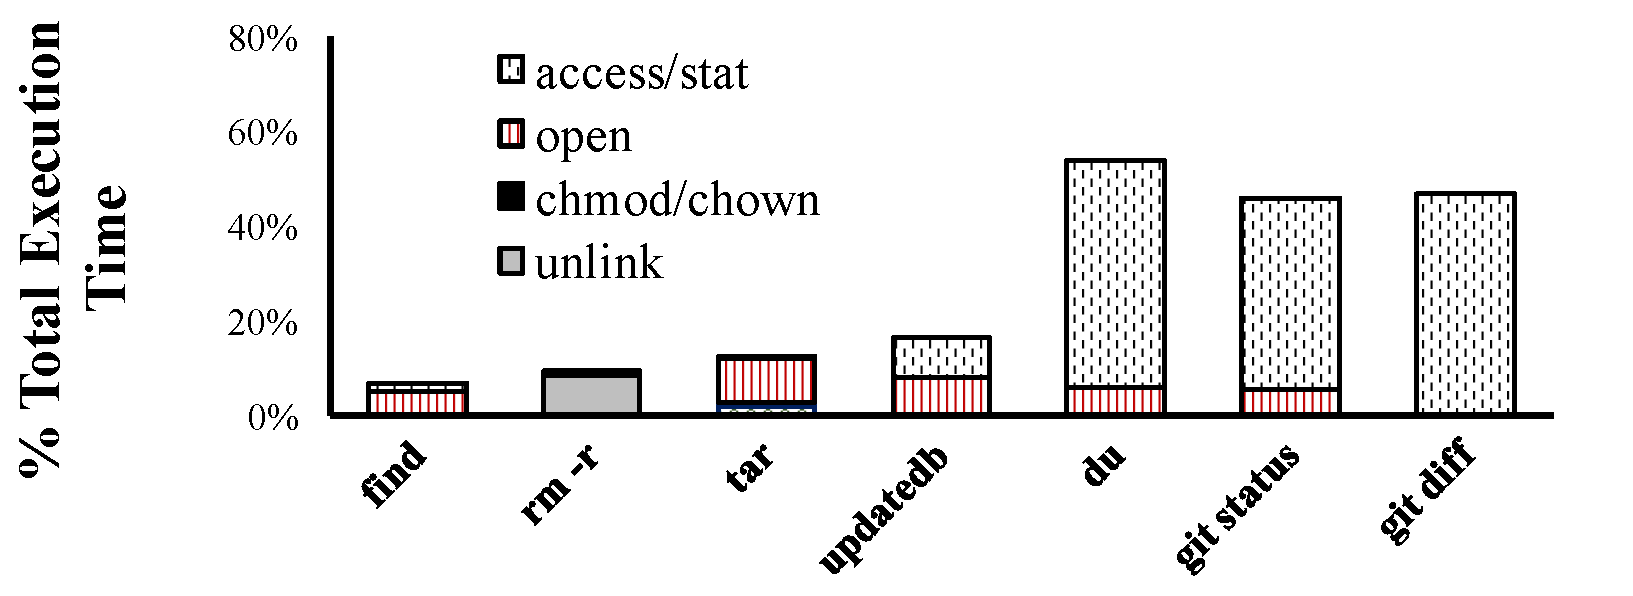
\includegraphics[width=5in]{dcache/plots/syscall-percentage.pdf} \\
\caption[Fraction of execution time on path-based system calls.]
{Fraction of execution time in several common utilities spent
executing path-based system calls with a warm cache, as measured with ftrace.}
\label{fig:dcache:lookup-frac}
%\vspace{-10pt}
\end{figure}

%\fixmedp{Please check these \% against time.  I think git diff is too high.  git status seems ok.}

Directory caches are essential for good application performance.
%Unix was designed such that ``(almost) everything is a file'',
%thus even accesses to in-memory file systems, device files, FIFOs and domain sockets
%first pass through the directory cache.
%In other words, 
Many common system calls must operate on file paths,
which require a directory cache lookup.
For instance, between 10--20\% of all system calls in the iBench system call traces do a path lookup~\citep{filenotafile}. 
Figure~\ref{fig:dcache:lookup-frac} lists the fraction of total execution time
%, as well as system time, 
several common command-line applications spend executing path-based system calls
(more details on these applications and the test machine in \S\ref{sec:dcache:eval}).
We note that these system calls include work other than path lookup,
and that these numbers include some instrumentation overhead;
% are coarse measurements that include  and work than path lookup;
%, and includes some time 
%for synchronous I/O (e.g., during {\tt rename}) as well as non-path tasks (e.g., creating 
%a file handle as part of {\tt open});
nonetheless, in all cases except {\tt rm},
the system call times and counts are dominated by
{\tt stat} and {\tt open}, for which 
%can be serviced from cache and for which 
path lookup is a significant component of execution time.
For these applications, path-based system calls account for 6--54\% of total execution time.
%and 25--77\% of system time.  
This implies that
lowering path lookup latency is
 one of the  biggest 
opportunities for a kernel to improve these applications' execution time.




\begin{figure}[t!]
\centering
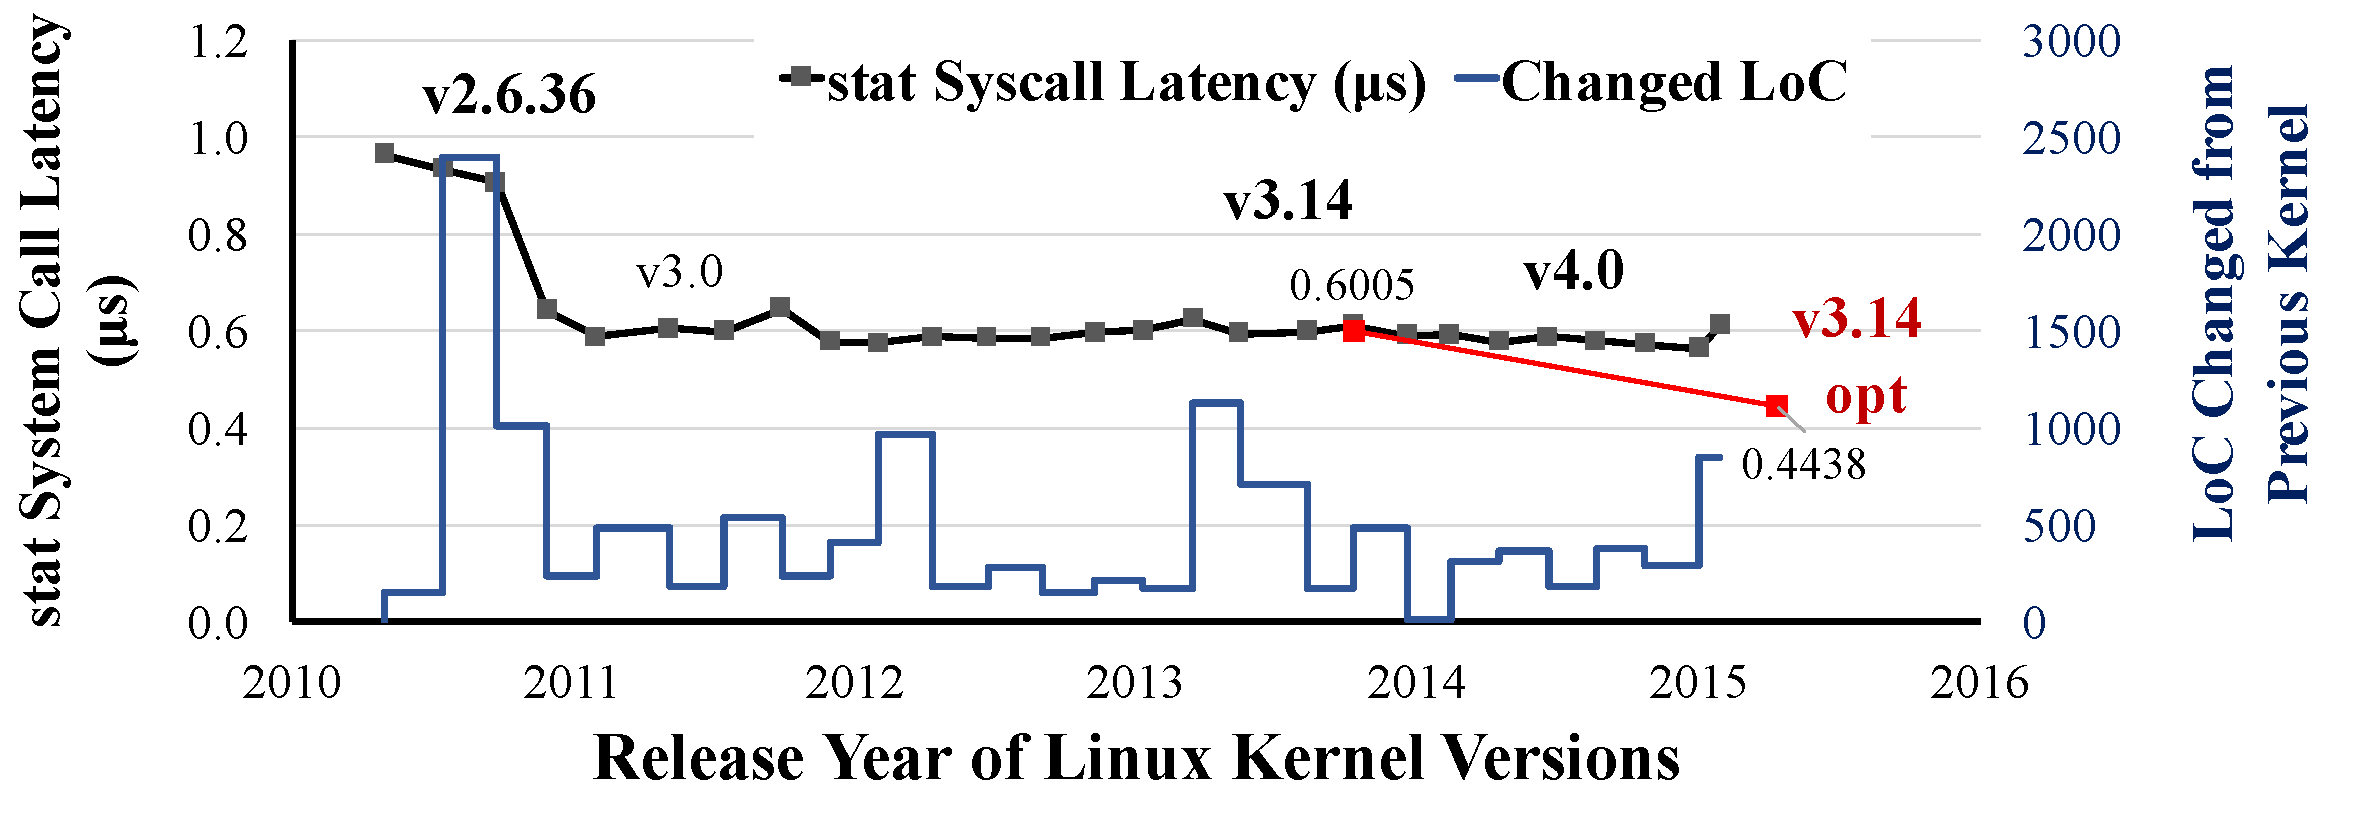
\includegraphics[width=6in]{dcache/plots/latency-by-version.pdf}
\footnotesize
\caption[Lantecy of {\tt stat} system call over years.]
{Latency of {\tt stat} system call with a long path {\tt XXX/YYY/ZZZ/AAA/BBB/CCC/DDD/FFF} on Linux over four years (lower is better), as well as the churn within the directory cache code (all insertions in {\tt dcache.c}, {\tt dcache.h}, {\tt namei.c}, {\tt namei.h} and {\tt namespace.c}). 
%Our optimizations significantly improve performance that has otherwise plateaued, despite significant ongoing developer effort.  
Our optimized \linuxver{} kernel 
further reduces {\tt stat} system call latency by \statspeedup{}\%.}
%\vspace{-15pt}
\label{fig:dcache:by-version}
\end{figure}


%\fixmedp{Add more evidence of lookup importance here: For instance, fraction of lookup time in file-related syscalls, or total lookup time in applications bound on file lookup latency.  }
Unfortunately, even directory cache hits are costly---0.3--1.1 \us{} for a {\tt stat} on our test Linux system, compared to only .04 $\mu$s for a {\tt getppid} and 0.3 \us{} for a 4 KB {\tt pread}. 
%\fixmetsai{Don, check this, I think read will be a better example, getppid is too trivial.}
This issue is taken particularly seriously in the Linux kernel community, which has 
made substantial revisions and increasingly elaborate optimizations to reduce the hit cost
of its directory cache, such as removing locks from the read path or replacing lock ordering with deadlock avoidance in a retry loop~\citep{corbet09jls,dcache-rcu}.
Figure~\ref{fig:dcache:by-version} plots directory cache hit latency against  lines of directory cache code changed 
over several versions of Linux, using a path-to-inode lookup \microbench{} on the test system described
in \S~\ref{sec:dcache:eval}.
These efforts have improved hit latency by 47\% from 2011 to 2013, but have plateaued
for the last three years.
%\fixmedp{if time, filter irrelevant changes from code deltas}
%at the cost of substantial developer effort.
%This latency appears to have plateaued 

The root of the problem is that the POSIX path permission semantics
seemingly require work that is linear in the number of path components,
and severely limit the kernel developer's implementation options.
%The root of this problem is that current directory cache
%designs reflect a straightforward implementation of the POSIX specification,
%which would seemingly require work that is linear in the number of path components.
For instance, in order to open file {\tt /\fnone{}/\fntwo{}/\fnthree{}} 
%for reading, 
one must have search permission
to parent directories {\tt /}, {\tt /\fnone{}}, and {\tt /\fnone{}/\fntwo{}},
as well as permission to access file {\tt \fnthree{}}.
The Linux implementation %of this specification is straightforward, 
simply walks the directory
tree top-down to check permissions.  
Unfortunately, when the critical path is dominated by 
walking a pointer-based data structure, 
including memory barriers on some architectures for multi-core consistency, 
modern CPUs end up stalling on hard-to-prefetch loads.
Moreover, because so many Linux features are built around this behavior, such as Linux Security Modules (LSMs)~\citep{wright+lsm},
namespaces, and mount aliases, it is not clear that any data-structural enhancements
are possible without breaking backward-compatibility with other Linux kernel features.
A priori, it is not obvious that a faster lookup algorithm, such as a single hash table lookup, 
can meet these API specifications and kernel-internal requirements; to our knowledge,
no one has tried previously.

%This paper proposes a decomposition of the directory cache, which allows
%most lookup operations to execute with a single hash table lookup (\S\ref{sec:dcache:dcache}),
%as well as optimizations to reduce the miss rate based on information that is {\em already in the cache}, but not used effectively (\S\ref{sec:dcache:readdir}).
%Our design maintains compatibility (\S\ref{sec:dcache:generalize}) through 
%several essential insights, including 
%how to separate the indexing of paths from checking parent permissions,
%and how to effectively and safely memoize the results of access control checks.


%% This paper proposes several new ways to organize a directory cache, which can yield 
%% substantial performance improvements over the current state of the art.
%% %This paper demonstrates that, despite this developer effort, there is still a substantial 
%% %missed opportunity hiding behind historical, intuitive, but not fundamental design choices.
%% Most of the Linux directory cache design reflects a straightforward implementation of the POSIX 
%% specification. %, with a division of labor that is suitable for mainstream file systems.

%This paper presents an alternative directory cache organization, which 
%improves performance by separating logical tasks, such as separating path indexing from permission checking; yet the design is sufficient to retain compatibility with POSIX.
%In the case of path lookup, 
%this paper demonstrates how 
%a per-component tree walk can be replaced with a single hash table lookup (\S\ref{sec:dcache:dcache}).
% without violating POSIX compliance.

%Our optimizations improve the performance of frequent lookup operations, but 
%introduce several costs, described in \S\ref{sec:dcache:dcache} and measured in \S\ref{sec:dcache:eval},
%which  we believe are acceptable and a net improvement for applications.
%First, these optimizations slow down infrequent modifications to the directory hierarchy, such as {\tt rename}, {\tt chmod},
% and {\tt chown} of a directory. 
%However, these slower operations
%account for less than .01\% of the system calls in the iBench traces~\citep{filenotafile}.
%Second,  the memory overheads of the dcache are increased.
%%(45\% per \dentry{}, as well as some  in our prototype).
%%(\fixmedp{XX MB} in our tests).  
%Third, lookup has a 
%probability of error from signature collisions that can be adjusted to be negligible
%%($2^{-141}$ in our configuration), 
%and within acceptable thresholds widely used by data deduplication systems~\citep{Debnath:2010:CSU:1855840.1855856, Srinivasan:2012:ILI:2208461.2208485, Quinlan:2002:VNA:645371.651321, Zhu:2008:ADB:1364813.1364831}.
%%, as well as how to remove
%%all memory barriers from the lookup path (\S\ref{sec:dcache:update}).
%In the micro-benchmark of Figure~\ref{fig:dcache:by-version}, our directory cache 
%optimizations improve lookup latency by 
%%revisions improve latency of accessing a long path
%%by 
%\statspeedup{}\% over unmodified Linux.
%%Our design addresses other missed
%%opportunities, such as identifying new opportunities to reduce the miss rate
%%through caching directory completeness.
%%\fixmedp{Do we want to highlight LoC?  3K is more than anything in the graph} \fixmetsai{Probably just mention in the evaluation. It's a metric that we should provide, but it's not awfully interesting.}
%%The total lines of code changed are fewer than 3,000 out of \fixmedp{XX}.
%%\fixmedp{Can we get 
%%, yet changes fewer than 3,000 lines of code.

%% SOSP cut - kind of long-winded
\begin{comment}
This paper rethinks current Linux directory cache design choices in light of the following goals:
\begin{compactitem}
\item {\bf Minimize the cost of a cache hit.} (\S\ref{sec:dcache:dcache}).
This means maximizing the benefit of temporal locality for frequent operations,
while pushing extra work of consistency maintenance onto less frequent, already-expensive operations.
%such as handling cache miss or updating massive metadata,
%in order to improve very frequent operations.
\item {\bf Maintain legacy compatibility.} (\S\ref{sec:dcache:generalize}).  Unix path semantics are complex, required by applications, file systems, and security modules, frustrating otherwise straightforward optimizations.  However tempting it may be to redesign path behavior to facilitate caching, path operations must exhibit the same behavior, with lower latency.
\item {\bf Never miss the same request twice in quick succession.} (\S\ref{sec:dcache:readdir}).  A number of less-frequent operations, such as reading a directory or secure temporary file creation, always miss in the cache {\em even if enough information is in cache to satisfy the operation.}  
%Of course, infrequent accesses should still be subject to a cache replacement policy, such as LRU.
\end{compactitem}
%Although directory caches must implement more complex semantics than a hardware memory cache,
%these principles should seem familiar to the reader with a basic architecture background.
%sadly, the Linux directory cache design violates all three.
\end{comment}

%This paper introduces several techniques to improve the performance of a directory cache,
%This paper explains several practical directory cache optimizations,
This paper demonstrates that these techniques improve performance for applications that use the directory cache heavily,
and the harm is minimal to applications that do not benefit.
%and that the worst case \microbench{} is only 12\% slower within \fixmedp{XX}\% of unmodified Linux.
%Each optimization we describe improves performance in isolation, and all can be combined.
%These optimizations change very few lines of code, and are backward-compatible with 
%legacy applications.  
%These changes are encapsulated in the VFS---individual file systems do not have to change their code.
%This paper describes a  prototype of these improvements implemented in Linux \linuxver{}.
%\S~\ref{sec:dcache:background} explains that the directory cache structure of Mac OS X, FreeBSD, and Solaris 
%are sufficiently similar that these principles should generalize.
%we compare and contrast Linux's directory cache
%with Mac OS X, FreeBSD, and Solaris in \S\ref{sec:dcache:background}, and explain inline how each
%optimization could be generalized to these other OS kernels.





%% \item {\bf Modularization and stackability}:
%% Any changes or optimizations must be implemented as modules inside Linux's VFS,
%% and can be stacked on top of the original design or any future optimizations. 
%% \item {\bf Backward compatibility}:
%% Any changes or optimizations must maintain least requirement of modifying any
%% file systems.
%% \item {\bf Generalization to other OSes}: Any changes or optimizations must be portable to other OSes with reasonable effort and change of design.




%% \dcache{} is proven to be effective on improving storage performance.
%% Experiments shows that,
%% in a Linux 3.x kernel, a \dcache{} with a xxx\% hit rate can speed up
%% metadata lookup and fetching time by xxx times.
%% \fixmetsai{experiment result, Linux version, and fs specs here}
%% However, we observed that Linux maintainers have made
%% constant and non-trivial efforts to improve \dcache{} in the Linux kernel.
%% We studied all \dcache{}-related source files in the Linux kernel Git repository,
%% and discovered that maintainers have committed
%% on average xxx revisions per source files.

%% We tested metadata lookup time on primary \dcache{}-related revisions.
%% Most changes on \dcache{} system only create xxx\%-xxx\% speed-up
%% than their predecessor.
%% \fixmetsai{result and graph here}.
%% Moreover, improvement to \dcache{} is still work-in-progress
%% for Linux maintainers.
%% \fixmetsai{reference to threads for latest dcache discussions}. 
%% All the evidences show that,
%% despite of significant reduction of storage operations,
%% efficiency of \dcache{} system internally still remains as a concern.

%% We argue that the design of \dcache{} needs to be carefully re-examined,
%% to fundamentally identify any missed opportunities that
%% improve value of \dcache{}.
%% At a high level, most optimization works for \dcache{} are focused on
%% improving ``how to cache'',
%% but we want to also lay eyes on ``what to cache'',
%% to ensure any valuable information returned from file systems
%% be captured by \dcache{} system.

%The contributions of this paper are as follows:
%\begin{compactitem}
%\item A performance analysis of the costs of path lookup and the opportunities
%to improve cache hit latency.
%\item A directory cache design that improves path lookup latency with a combination of techniques, including:
%  \begin{compactitem}
%  \item Indexing the directory cache by full path, reducing average-case lookup from linear to constant in the number of path components.
%  \item A Prefix Check Cache (PCC) that separates permission checking from path caching.  The PCC memoizes permission checks, and is compatible with LSMs~\citep{wright+lsm}.
%  \item Reducing the cost of checking for hash bucket collisions with path signatures.
%  \end{compactitem}
%\item Identifying opportunities to leverage metadata the kernel already has to reduce miss rates, such as tracking whether a directory is completely in cache.
%\item Carefully addressing numerous, subtle edge cases that would frustrate rote application of these techniques, such as integration with symbolic links and Linux namespaces.
%\item A thorough evaluation of these optimizations.  For instance, our optimizations improve throughput
%of the Dovecot IMAP server by up to \dovecotspeedup\% and latency of 
%updatedb by up to \updatedbspeedup{}\%.
%%git version control system by up to 25\%.
%
%\end{compactitem}

%\section{Background}
\label{sec:background}

This section summarizes \sgx{},
and current design points for running or porting applications on \sgx{}.
%and the legacy frameworks of porting 
%including \haven{}~\cite{baumann14haven}, \scone{}~\cite{osdi16scone}, and Panoply~\cite{shinde17panoply}. 


\subsection{Software Guard Extensions (SGX)}
\label{sec:background:sgx}

%\begin{figure}[t!]
%\centering
%\includegraphics[width=\linewidth]{figures/libosvssdk.pdf}
%\footnotesize
%\vspace{-0.3in}
%\caption{
%Comparison between libOS-based model (e.g., \haven{} and \graphenesgx{})
%and SDK-based (SDK for \sgx{}) model for migrating applications in enclaves.
%Green (light) boxes are trusted components and red (dark) boxes are untrusted.
%The libOS-based model often yields a larger TCB in the enclave,
%while the SDK-based model requires developers to be responsible of
%securing the enclave on the untrusted interface.
%}
%\label{fig:libosvssdk}
%\end{figure}

The primary SGX abstraction is an \emph{enclave}: an isolated execution environment within the virtual address space of a process.
The code and data in enclave memory do not leave the CPU
package unencrypted; when memory contents are read back into cache,
the CPU decrypts the contents, and checks the integrity of cache lines and the virtual-to-physical mapping.
SGX also cryptographically measures the integrity of enclaves at start-up, and 
provide attestation to remote systems or other enclaves.
%Remote entities can identify the owners of enclaves by distinguishing the cryptographic measurements
%generated with different signing keys.

%%% \sgx{} is a new feature on the 6th-genaration \intel{} CPUs.
%%% it contains a set of new x86/64 instructions, to initiate, destroy, and attest isolated execution environments (i.e., enclaves) in the address space of applications.
%%% When \sgx{} loads an application in an enclave,
%%% the code and data of the application will remain encrypted in the main memory,
%%% forbidding any mean to eavesdrop the application secrets.
%is a set of new x86/x64 instructions introduced
%to the latest \intel{} CPUs,
%to bootstrap an isolated execution environment
%inside applications' virtual memory address space.
%\sgx{} creates a memory region
%(generally referred as {\bf enclave}), storing both the code and data of the isolated execution,
%which stays encrypted in DRAMs and only the CPU is capable of encryption and decryption.
%The CPU derives the encryption key
%from the cryptographic measurement of the initial state of enclave memory,
%to allow remote entities to verify the soundness of execution and establish the trust
%needed for provisioning sensitive data.

\sgx{} enables a threat model where one only trusts the \intel{} CPUs and the 
code running in the enclave(s).
%whereas the rest of application, system software, off-CPU-package hardware devices and providers are untrusted. 
\sgx{} protects applications from three different types of attacks on the same host, which are summarized in Figure~\ref{fig:sgx-threats}: untrusted application code inside the same process but outside the enclave; operating systems, hypervisors, and other system software;
%\fixme{added Mona's suggestion}
other applications on the same host; and off-chip hardware.
A SGX enclave can also trust a remote service or enclave, and be trusted after inter-platform attestation~\cite{sgx-attestation}.




%%% \begin{compactenum}

%%% \item {\bf Inside process memory:}
%%% \sgx{} partitions the application process into two privilege levels, as the trusted part (in enclaves) which can access the whole process memory, and the untrusted part (outside enclaves) forbidden to access enclave memory.
%%% %the privileged part (in the  enclave region) can access all process memory,
%%% %while the unprivileged part (outside the enclave region) is limited to access only data that are not isolated by \sgx{}.

%%% \item {\bf From hosting OSes or hypervisors:}
%%% \sgx{} assumes that OSes and hypervisors can be compromised by either exploiting system vulnerabilities
%%% or malicious system software installed by administrators.
%%% Both types of compromise are legitimate threats to modern OSes, due to complexity of modern OSes and usage of public facilities like clouds.

%%% %Operating systems or hypervisors
%%% %that are either compromised by rootkits
%%% %or deliberately modified by the host providers.
%%% %An attacking host can access the raw data in DRAMs, or remap the
%%% %physical pages to other contexts.

%%% \item {\bf Physically from the hardware:}
%%% One type of attacks that cannot be defended by software-based solutions~\cite{flicker, criswell2014virtualghost}
%%% is from the attackers who have physical access to the hosts.
%%% \sgx{} can resist attacks on the host hardware
%%% including hacking peripheral devices like ethernet cards and connectors~\cite{hudson15thunderstrike}, tapping into buses, or eavesdroping DRAM data using Cold-boot attack~\cite{halderman09coldboot}.


%%% \end{compactenum}


%%% \sgx{} protects an application against unpredictable threats from both local and remote hosts.
%%% \sgx{} establishes a trusted path
%%% from one enclave to another,
%%% providing end-to-end protection to both enclaves to
%%% exchange data with confidentiality and integrity.
%%% %, processing the data and returning the computation results with end-to-end protection.
%%% We can further divide up the protection using \sgx{} into three elements:
%The use cases of \sgx{} mostly involve the process that an enclave
%retrieves a signed attestation from the processor,
%to exchange provisioning of critical information from remote servers.
%The purpose of such process is equivalent to
%expanding the trusted execution
%from remote servers
%to untrusted hosts,
%to harness resources such as CPU cycles and DRAMs.

%%% \begin{compactenum}

%%% \item {\bf Isolated execution:}
%%% \sgx{} guarantees the execution initiated in an enclave
%%% to be isolated from any part of the system except the enclave itself.
%%% %any part of the system except the enclave itself can access the execution state. 
%%% Achieved by the secrecy of encryption keys in \intel{} CPUs.

%%% \item {\bf Attestation of integrity:}
%%% Remote entities with a \sgx{}-enabled CPU can verify the integrity of an enclave, using the \intel{} Attestation Services (ISV)~\cite{isv}.
%%% %for its integrity of running the exact code that it is given.
%%% Achieved by the uniqueness of CPU keys to sign the cryptographic measurement of enclaves.

%%% \item {\bf Authentication:}
%%% Remote entities can identify the owners of enclaves by distinguishing the cryptographic measurements generated with different signing keys.


%%% %explicitly launched for processing the specific tasks, regardless of the identicality of execution.
%%% %That is, two mutually distrusting users can launch the same execution in  separate enclaves, yet be able to distinguish by the measurements as MACs (Message Authentication Code) signed by the users' private keys.

%%% \end{compactenum}


%One must note that \sgx{} only promises the integrity of application binaries
%initially loaded in enclaves.
%The gap between integrity of binaries and complete security has to be filled
%by ones who develop and approve the applications.
%More specifically, the clients are responsible of
%testing whether the applications contain any vulnerabilities
%that lead to information leak.
%To minimize the risk of leaving any flaws in the applications unintentionally,
%developers often tend to cut down the trusted computing base (TCB)
%of the applications. With smaller TCB, clients who launched the enclaves
%can more easily reason about the thoroughness of securing the execution.

%To achieve smaller TCB, the software development kit of \sgx{}
%intends to encourage developers to partition the applications and
%keep only security sensitive components in the enclaves.
%Such an intention is exactly contradicted by the trust model of \haven{},
%which must trust the loaded application as a whole.
%Except for the cases in which the whole applications must be secured,
%\haven{} actually downgrades the trustworthiness of enclaves.
%Figure~\ref{fig:libosvssdk} shows the comparison of the two models.


%%% By synthesizing and streamlining these three elements (i.e., isolation, attestation and authentication),
%%% \sgx{} provides a promising build block to securing applications
%%% from unpreditable security threats.

%developing applications
%that are resistant to unpreditable, unavoidable threats.
%Users expect \sgx{} to build up a wall for protecting the sensitive data, even against a catastrophic scenario like a complete takeover of the infrastructure.  

%\fixmedp{Explain how to read the figures in the captions. What do colors and shading mean?}
%
%\fixme{Disabled the whole discussion about SDK. dp: ok with me, but probably drop from figure} 
\begin{comment}
\subsection{The legacy framework (The \sdk{})}

{\bf Intel's \sgx{} SDK} (software development kit) for Linux~\cite{intel-sgx-sdk} is the official framework
for programming \sgx{} execution within Linux applications.
\sdk{} includes the components of two phases:
a {\bf compile-time utility} to generate a valid executable for running inside enclave,
and a {\bf run-time framework} to trigger the hardware-enforced isolated execution.
The two-phased design is based on the assumption that compilation of applications
is controlled by trusted, security experts,
to retain the trustworthiness of isolation model when running on untrusted OSes.


The work flow of \sgx{} programming using \sdk{} is as follows:
\begin{compactenum}
\item At the build-time (on trusted hosts), developers create a self-contained, static executable as the initial code and data after enclave creation.
We refer the executable as an ``enclave image''.
The enclave image is statically links with the enclave infrastructure, which provides enclave APIs (e.g., retrieving attestation) and a extremely small set of POSIX functions (e.g., {\tt memset()}).
After linking, the compile-time utility signs the executable and inserts the enclave signature structure
({\tt SIGSTRUCT}) in the application code.
\item At the execution-time (on untrusted hosts), the enclave image is taken by the framework. The user-space driver then requests enclave creation with the kernel driver, through {\tt ioctl()} to a pseudo-device {\tt /dev/isgx}.
The kernel driver creates and initializes an enclave using the authenticated signature structure,
and a token exchanged from an architectural enclave, {\tt AESMD}, for ensuring the validity of enclave. 
\end{compactenum}





%During the compile time,
%the developers create a self-contained, static binary, as the initial image of an run-time enclave (an ``enclave image'').
%\sdk{} provides the infrastructural libraries (libsgx) for static linking, which contain enclave APIs and few POSIX functions.
%A signing tool of \sdk{} will generates a valid enclave signature
%derived from the enclave image.
%Both the static linking and signing must happen on a trusted, development machine.


%After generating the enclave image, developers then ship it with the rest of application,
%to untrusted hosts (\sgx{}-enabled)
%where the \sdk{} run-time framework is installed.
%The run-time framework provides both kernel and user-space drivers,
%to interface \sgx{} hardware using the new x86 instructions (e.g., {\tt ECREATE}, {\tt EADD}, {\tt EENTER}).
%The framework also includes an architectural enclave (AESM), for validating the enclave attributes (and generating a run-time token),
%and a kernel EPC (enclave page cache) driver that manages paging for all running enclaves.



% includes both compile-time and run-time components:
%for the compile time, the SDK provides all the infrastructure libraries,
%which the applications statically link with,
%and a signing tool that generates the enclave signatures for hardware validation.
%The run-time framework then takes the signed enclave binaries,
%and uses the kernel and user-space drivers to initiate the isolated execution in enclaves.



\sdk{} centers the whole programming model based on the concept of partitioning an application,
and isolating only minimum application code in enclaves.
The partitioning minimizes the risk of compromising the enclaves,
due to smaller trusted computing base (TCB) and less opportunity of omitting security glitches.
With this model,
developers are expected
to identify the part of an application that performs the sensitive operations,
and define an validated interface to
the sensitive part and rest of the application.
\sdk{} encourages partitioning by reducing the difficulty of defining and accessing the interface---a language tool automatically generates the interface code with extra argument-sanitizing code.
The generated interface code essentially filters input and output of the enclave,
and prevents randomly copying memory across the enclave boundary, leaking or corrupting internal data.


%The Intel SDK has its limitations. The infrastructure of the SDK provides APIs in enclaves for accessing SGX features (e.g., attestation), as well as a small set of POSIX APIs
%(\roughly{}10 functions, such as {\tt printf} and {\tt memset}).


Despite that \sdk{} attempts to alleviate the difficulty of partitioning for SGX,
porting a piece of application code that is sophisticated and interactive to the rest of application
is still a significant cost to pay.
In general, developers want to find a reasonable granularity of partitioning---a ``sweet spot'' that partitions the application code neither too small nor too large, 
to nicely balance between frequency of enclave exits and risk of introducing incompatible code.
For an application written in C/C++, partitioning is cumbersome especially if the application is poorly modularized.


Unfortunately, the limited POSIX support in the \sdk{} infrastructure really strikes
the opportunity of fine-grained partitioning.
The lack of POSIX APIs in the infrastructure is fundamental, due to the restriction
on OS interaction from the enclaves.
The missing APIs encapsulates system calls, which can expose the enclave to some risky OS interaction model, such as {\bf Iago Attacks}~\cite{checkoway13iago}.

%In conclusion, this work targets on completing the API support, either at POSIX level or system calls,
%while retaining the isolation model.
%The platform can assist developers to refocus on partitioning applications for minimizing the risks.

\end{comment}

\subsection{SGX Software Design Space}

This subsection summarizes the principal design choices facing any 
framework for running applications on SGX.  We explain the decisions in
recent systems for SGX applications, and the trade-offs in this space.

\begin{figure}[t!]
\centering
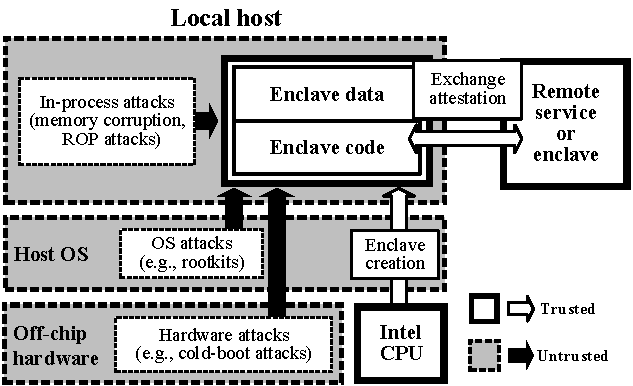
\includegraphics[width=.5\linewidth]{sgx.pdf}
\caption{The threat model of \sgx{}. \sgx{} protects applications
from three types of attacks:
in-process attacks from outside of the enclave,
attacks from OS or hypervisor, and attacks from off-chip hardware.}
% Red (dark) boxes are untrusted components and green (light) boxes are trusted.}
%For each enclave, \sgx{} establishes the chain of trust from the \intel{} CPU.
%Enclaves across physical machines or even infrastructures can remotely attest the integrity of execution, using the signatures generated and signed by the CPU.
%Green (light) boxes and arrows represent the trusted components and operations, and red (dark) boxes and arrows represent the otherwise.
\label{fig:sgx-threats}
\end{figure}

\paragraph{How much functionality to pull into the enclave?}
At one extreme, a library OS like Haven~\cite{baumann14haven} pulls most
of the application-supporting code of the OS into the enclave.
On the other extreme, thin ``shim'' layers, like SCONE~\cite{osdi16scone} and Panoply~\cite{shinde17panoply} 
wrap an API layer such as the system call table.
Pulling more code into the enclave increases the size of the TCB,
but can reduce the size and complexity of the interface, and attack surface, 
between the enclave
and the untrusted OS.

The impact of this choice on performance
largely depends on two issues. First, entering or exiting the enclave 
is expensive; if the division of labor reduces enclave border crossings, 
it will improve performance.
The second is the size of the Enclave Page Cache (EPC),
limited to 128MB on version 1 of SGX.
If a large supporting framework tips the application's working set size
past this mark, the enclave will incur expensive swapping.


\paragraph{Shielding complexity.}
SGX hardware can isolate an application from an untrusted OS, but 
SGX alone can't protect an application that  requires
functionality from the OS.  {\em Iago attacks}~\cite{checkoway13iago}
are semantic attacks from the untrusted OS against the application, where an unchecked system call return 
value or effect compromises the application.
Iago attacks can be subtle and hard to comprehensively detect, at least with the current
POSIX or Linux system call table interfaces.

Thus, any SGX framework must provide some {\em shielding} support, to 
validate or reject inputs from the untrusted OS.  
The complexity of shielding is directly related to the interface complexity:
inasmuch as a library OS or shim can reduce the size or complexity of the 
enclave API, 
the risks of a successful Iago attack are reduced.

\paragraph{Application code complexity.}
Common example applications for SGX in the literature 
amount to a simple network service running a TLS
library in the enclave, putting minimal demands on a shim layer. 
Even modestly complex applications, such as the R runtime and a simple
analytics package, require dozens of system calls providing wide-ranging functionality, 
including \syscall{fork} and \syscall{execve}.
For these applications, the options for the user or developer become: 
(1) modifying the application to require less of the runtime; (2) opening and shielding more 
interfaces to the untrusted OS; (3) pulling more functionality into a shim or a library OS.
The goal of this paper is to provide an efficient baseline, based on (3),
so that users can quickly run applications on SGX, and developers can 
explore (1) or (2) at their leisure.

\paragraph{Application partitioning.} An application can have multiple
enclaves, or put less important functionality outside of the enclave.
For instance, a web server can keep cryptographic keys in an enclave,
but still allow client requests to be serviced outside of the enclave.
Similarly, a privilege-separated or multi-principal application might create a separate enclave for
each privilege level.

This level of analysis is application-specific, and beyond the focus of this paper.
%which is on running unmodified applications in enclaves.
However, partitioning a complex application into multiple enclaves
can be good for security. In support of this goal,
\graphenesgx{} can run smaller pieces of code, such as a library, in an enclave, as well as
coordinate shared state across enclaves.

%* Partitioned vs. unpartitioned app?

%** Right choice depends a lot on whether the app has multiple principals or security concerns.

\begin{comment}
\fixmedp{Did a first cut at 2.2; needs to integrate the figure (or drop it).  I didn't know what to write for 2.3 yet.  I left the old text below for now (if there is anything you really want to save), but it needs to go away}

\subsection{Open Challenges}

\fixmedp{Here, I would give a taste of some of the issues we solve and why they are hard, like dynamic loading (and maybe fork or IPC).  Keep it short, a few paragraphs.}
\end{comment}

%\begin{figure}[t!]
%\centering
%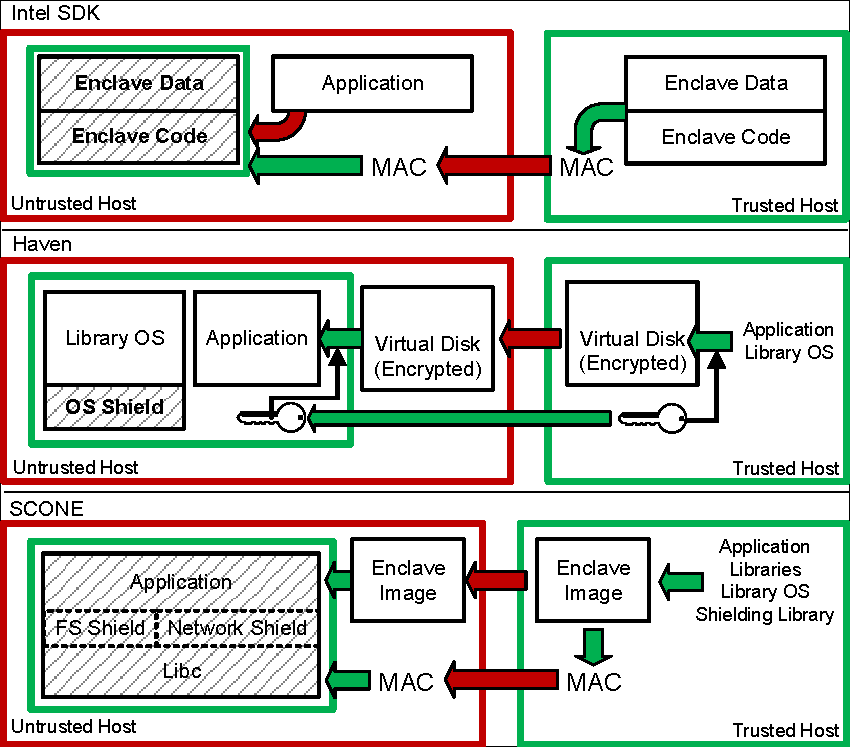
\includegraphics[width=\linewidth]{figures/sdkvslibos.pdf}
%\caption{Comparison of the code integrity model among different \sgx{} frameworks, including the \sdk{}, \haven{} and \scone{}.}
%%Green (light) boxes and arrows represent the trusted components
%%and operations, and red (dark) boxes and arrows represent the otherwise.
%%Patterned blocks represent the code and data included in the initial measurements of the enclaves.}
%\label{fig:sdkvslibos}
%\end{figure}


\begin{comment}
\subsection{\sgx{} shielding systems}
\label{sec:background:shielding-systems}




The current \sgx{} shielding systems, such as \haven{}~\cite{baumann14haven}, \scone{}~\cite{osdi16scone}, and Panoply~\cite{shinde17panoply}, enforce end-to-end isolation to
legacy applications without partitioning.
A \sgx{} shielding system preserves the trusted computing base (TCB)
of an application, and further increases it with a shielding layer to defend against the untrusted OSes.
By avoiding application partitioning,
%model of quarantining an unmodified, COTS application in an \sgx{} enclave.
a shielding system minimizes the effort of reprogramming the applications for \sgx{} execution, often with recompilation or packaging the binaries in an encrypted enclave.
%to merely recompiling or packaging the application code before signing it off for enclave execution.
%These \libos{}es internalize OS features into the enclave, to maintain a fixed-size,
%narrow interface to the untrusted host OSes.
%Porting applications using a \sgx{} \libos{} is vastly different from the programming model of \sdk{}---no programming effort is needed when porting with a \sgx{} \libos{}, and applications are isolated without partitioning.
In the following paragraphs, we compare the current shielding systems with the \graphenesgx{} approach.

\haven{}~\cite{baumann14haven} uses a \libos{} called \drawbridge{} in each enclave
to shield a single-process \emph{Windows} application from the untrusted host OS.
\haven{} absorbs the implementation of system APIs (i.e., Win32 APIs) from the host OS,
%\haven{} uses \drawbridge{}~\cite{porter11drawbridge} as the backbone of its enclave infrastructure, 
and exports a narrow enclave interface on which untrusted inputs are carefully filtered to defend against the Iago-type attacks.
Adding a \libos{} to each enclave causes a bloat of TCB---for \haven{}, the size of a \libos{} binary and shielding layer is \roughly{}200MB.
\haven{} has to establish the trust and integrity in all these binaries loaded into an enclave. Except that the shielding layer is a part of the enclave since its creation, \haven{} enforces the integrity of both the \libos{} and the isolated application,
by storing all binaries on an encrypted virtual disk and relying a remote, trusted server to provision the key for decryption.
\haven{} builds a trusted path from a remote server to local cloud machines,
to securely bootstrap application execution inside the enclaves.
%Other minor comparison between \haven{} and this work: the development and evaluation of \haven{}, at publication, is based on a simulated architecture.
%On the contrast, \graphenesgx{} is a released open-source platform, tested by many developers from institutes and corporations. \fixme{maybe bring up TCB?}



\scone{}~\cite{osdi16scone} isolates Linux micro-services in enclaves as a container-like environment.
After a brief attempt of building a \libos{} like \haven{},
\scone{} chooses a different approach of shielding the system API usage in applications, by designing shielding strategies based on each API.
\scone{} stacks the application on top of file-system and network shielding libraries, and extends a standard library C (musl~\cite{musl}) to securely exit the enclave for system calls.
Within the \sgx{}-aware Libc, \scone{} carefully filters the inputs from the host system calls, as the defend against known Iago attacks.
For instance, \scone{} ensures that pointers given to and returned by a host system call will point to addresses outside the enclave,
to prevent the host OS to manipulate pointers and cause memory corruption in the enclave.
\scone{} also authenticates or encrypts file or network streams
based on configurations given by the developers.


%The \libos{} implementation in \scone{} is based on musl~\cite{musl} and LKL (Linux kernel library)~\cite{lkl}.
%The design of a SCONE enclave (or Secure Container) has similarity
%with a basic block of \graphenesgx{}:
%they both validate input files based on cryptographic methods, and are fully configurable at a per-file basis.
%However, \graphenesgx{} supports a more complete set of Linux system APIs.
%The APIs that \graphenesgx{} especially contributes over \scone{} are the Linux multi-process APIs, including copy-on-write {\tt fork()}, {\tt exec()}, signals, and system V IPC (message queues and semaphores).

Panoply~\cite{shinde17panoply} further reduces the TCB of a shielding system over the SCONE approach, by excluding both a \libos{} and \libc{} from enclaves.
Instead, Panoply uses a shim layer shielding a portion of the POSIX API. The shim layer yields about 20 KLoC as its TCB (trusted computing base), which is much smaller than libc and/or a library OS.
% in other shielding systems.
As Panoply delegates the libc functions outside the enclave, its shim library defends the supported POSIX API,
including 91 {\em safe} functions and 163 {\em wild (unsafe)} functions.
Panoply also supports multi-process API including \fork{}, \exec{}, signaling, and sharing untrusted memory with inline encryption.
Compared to \graphenesgx{}, Panoply has made some different design decisions in supporting multi-process API,
including supporting fork by copying memory on-demand with statically determining memory access,
and using secured messaging for inter-process negotiating instead of coordinating over an encrypted RPC stream.




\subsection{Comparison and security implications}

\fixme{need to drop the SDK discussion, revisit the security claims, and discuss Iago attacks in details.}

Figure~\ref{fig:sdkvslibos} shows the comparison between \haven{}, \scone{}, Panoply, and \graphenesgx{}.
%The \sdk{} model uses a static MAC of the enclave code and data, given to the \sgx{} driver for bootstrapping the isolated execution.
The \haven{} model only initiates enclaves with the OS shield layer,
which unpacks the enclave binaries from a virtual disk---decrypted using a provisioned key.  
The \scone{} model extends the \sdk{} model---it statically links the application binaries with the shielding library, creating a static enclave image verifiable by its MAC. The \sdk{} and \scone{} model retain more flexibility in deploying and integrating \sgx{} enclaves by focusing on the code integrity rather than encryption.

The key concerns that affects users choosing among these solutions are {\bf trusted computing base (TCB) size} and {\bf attack surface}.
However, since all these solutions are based on different design decisions, assumption and requirements, the comparison of TCB size and attack surface is often imprecise and inconclusive.

\paragraph{TCB size.}
Most studies measure the TCB size of a system by the total LoC (lines of code) written for all the trusted components, or the size (in bytes) of all the trusted binaries.
The comparison of TCB size is only meaningful when two systems have comparable system features,
and are order-of-magnitude different in term of LoC or binary size.
For instance, the comparison of TCB size between \haven{} and \scone{} is never an apples-to-apples comparison.
The implemented system features and personalities
in these two systems are fundamentally different, and \haven{} supports a much larger fraction of Windows features than the fraction of Linux features supported by \scone{}.

We argue that the only occasion that the reduction of TCB size
can be convincingly demonstrated is when a design has partitioned a system into isolated components,
or removed unreachable execution paths.
For instance, the \sdk{} promotes application partitioning for \sgx{};
it requires additional partitioning effort but is effective for confining the TCB size.
By statically linking the application binaries
with the shielding layers and standard C library, \scone{} offers more opportunities in stripping the Libc and shield code of unused APIs, and thus reducing its TCB size.



\paragraph{Attack surface.}

Most studies estimate the severity of having an attack surface by the size of interface to the trusted and untrusted components.
The experience of \scone{} provides an important insight for estimating attack surface: the narrowness of interface is not proportional to the difficulty of defending against incoming attacks.
An interface overloaded with too many features or semantics can become a major source of vulnerabilities.

%\subsection{The \graphene{} Library OS}
%
%\graphene{}~\cite{tsai14graphene} introduces a \libos{} design that supports
%both single-process and multi-process Linux applications,
%but retains a narrow host interface (43 functions) as a vantage point for enforcing security isolation.
%The main contribution of \graphene{} is an distributed implementation of the POSIX namespace coordination,
%to support Linux multi-process abstractions across \libos{} instances.
%All the multi-process abstractions in \graphene{} is implemented using simple pipe-like RPC streams,
%without relying on any host memory sharing support.
%Based on this design, \graphene{} can easily isolate mutually untrusting applications,
%by blocking the RPC streams between unrelated applications.
%
%
%
%The design decisions made by \graphene{} are important keys to the \graphenesgx{} framework.
%First, the host interface contains mostly internal abstractions, and three external ones including files, network connections, and RPC streams.
%The simplicity of the host interface facilitates shielding the \libos{}
%from risky OS interaction.
%Moreover, \graphene{} implements multi-process abstractions across instances without memory sharing.
%\graphenesgx{} can rely on the distributed POSIX implementation
%to support multi-process applications across multiple enclaves, by coordination over validated RPC streams.


\end{comment}




\papersection{Background and Motivation}
\label{sec:background}

%\fixmets{1.5 page}

This section discusses the security features of  \sgx{}, and the challenges faced by developers that
intend to use \sgx{} for partitioning \java{} applications.
%the key challenges developers face when trying to manually partition applications using a technology such as \sgx{}.
%discuss the programming models and threats to security of \sgx{} enclaves.

\begin{figure}[t!]
\centering
\includegraphics[width=1.0\linewidth]{libosvssdk.pdf}
\footnotesize
\caption{
Comparison between the Non-partitioned model (e.g., Haven)
and partitioned model for protecting applications in enclaves.
Green (light) boxes are trusted components and red (dark) boxes are untrusted.
The non-partitioned model yields a larger TCB in the enclave,
while the partitioned model requires developers to determine the untrusted interface at the enclave boundary.
}
\label{fig:libosvssdk}
\end{figure}

\papersubsection{\sgx{} Enclaves}

\intel{} \sgx{} ({\it Software Guard Extensions})
are a set of new x86/x86\_64 instructions
introduced in the \intel{} Skylake processor family.
Using \sgx{}, an 
application can designate part of its virtual memory as an {\em enclave}.
The CPU ensures that the contents of the enclave never leave the CPU package unencrypted.
The CPU also measures the integrity of a binary loaded into the enclave, and offers remote attestation,
similar to a TPM~\cite{TPM}.

%%% create a protected memory region, called an {\em enclave}, inside it's virtual memory,
%%% where it can load its security sensitive data with hardware-enforced isolation from the untrusted OS. 
%%% The processor with \sgx{}
%%% guarantees that any data loaded in enclave
%%% stays encrypted in the DRAM, by using a secret key deterministically derived from the application's cryptographic measurement and the CPU secret. 

\sgx{} is an appealing tool for protecting small amounts of highly-sensitive data or code, because it can defend 
against a malicious or compromised OS, hypervisor, or even hardware peripheral.
For instance, Hoekstra et al.~\cite{sgx-workshop1} show how \sgx{} can be used
to build a trusted path from a video chat application to a GPU and network card, which maintains confidentiality and integrity of the
video stream, even if the OS is compromised.
Similarly, because DRAM contents are encrypted, \sgx{} can resist attacks such as cold-boot attacks~\cite{halderman09coldboot} or 
malicious peripheral devices~\cite{hudson15thunderstrike}.

%\fixmedp{The flow from here to partitioned apps doesn't make sense.  Why are we getting into \sgx{} problems, then partitioned vs non-partitioned, then back to more problems?}
\sgx{} provides useful building blocks for secure applications, but does not
absolve the programmer of all responsibility for reasoning about end-to-end security.
Bugs in the application or supporting libraries can still disclose sensitive data from an enclave,
and porting code into \sgx{} can be subtle.
Inputs and outputs of an enclave must be checked carefully, and application-internal functions 
may not be hardened to the level of network-facing application interfaces.

Fundamentally, this argues for some combination of static analysis
and runtime monitoring of 
enclave code.  This is greatly simplified when the enclave code is written in higher-level languages
with properties 
%amenable to analysis.
%with type safety, memory safety, and other 
%that provide important 
%safety properties,
such as type safety or memory safety. %, thereby reducing the likelihood of these vulnerabilities.
Ideally, one would formally verify security properties of enclave code~\cite{moat}; this verification is significantly aided by using 
higher-level languages amenable to formal reasoning.
%Verification is significantly harder
%with C/C++ or assembly languages.


%The rest of this subsection outlines several pitfalls in partitioning an application for \sgx{}.



%\paragraph{Side Channels and Denial-of-Service.}
%In the current \sgx{} design, side channels are a significant concern, and are out of the scope of this paper.
%A controlled channel attack~\fixmedp{cite} can single step enclave execution by inducing page faults
%in the enclave.  \sysname{} does not specifically defend against side channel attacks,
%and we expect that any solution to this problem involves redesigning the %division of labor in virtual
%memory management for enclaves.

%Similarly, there is no guarantee that a compromised application will ever %enter
%an enclave.  Denial-of-service attacks are out of scope for this paper.

%% \paragraph{Writes outside of the enclave.}
%% However, the security of \sgx{} enclaves is founded on trusting the code running inside the enclave.
%% \sgx{} allows the trusted code to read and write data structures 
%% outside of the enclave.  Thus, it is easy for a developer to inadvertently write
%% code that discloses a secret, say by using a library that memoizes intermediate results to the untrusted heap.
%% A fundamental requirement is that developers must be able to reason about (or assert)
%% what code can and can't access data {\em outside} of the enclave.
%% \fixmedp{Can we say anything about whether such tools exist before Civet?}

%% %\fixmedp{Do I recall correctly that you can easily write to data outside of the enclave?  If so, this seems like something easy to get wrong, especially 
%% %if a library memoizes intermediate results.  The developer needs to be able to tell 
%% %Unless I am full of shit, can we paragraph-ize this fixme?

%% \paragraph{Vulnerabilities in the isolated applications.} 
%% One of the major threats to enclave security is the vulnerabilities in the isolated code,
%% such as memory corruption bugs,
%% control flow or information flows, semantic bugs, and so forth. 
%% %Moreover, although \sgx{} code integrity guarantees make enclaves resistant to code injection,
%% %an attacker may still manipulate control flow using code-reuse attacks~\cite{code-reuse-attacks}.
%% Moreover, recent research~\cite{hudata} shows that even with control flow integrity,
%% attackers can still manipulate the execution to leak the secrets through information flow.



%%% \sgx{} also proves the integrity of loaded binaries to remote trusted entities
%%% using mutual attestation based on a symmetric key generated from the measurements of communicating entities.
%%% \sgx{} usage model mostly involve the launched enclave mutually attesting the trusted host
%%% to obtain provisioning of security-sensitive information
%%% through a trusted channel. Such an execution model leverages resources such as CPU and DRAM from vulnerable untrusted \sgx{}-enabled hosts owned by cloud providers
%%% by extending the trust from
%%% the hosts owned and trusted by the clients or service providers.
%%% For instance, \sgx{} can isolate the decoder engine in an enclave
%%% after authenticating the customers to enforce Digital Right Management (DRM) even if the digital data is hosted on an untrusted cloud server.

%Use cases of \sgx{} mostly involve the launched enclave
%retrieving a cryptographically signed attestation from the processor,
%to exchange security critical information with remote servers through secured channels.
%The effect is equivalent to expanding the trusted space from remote servers
%to the local end, to harness local resources such as CPU and DRAM.

%One must note that \sgx{} only promises the integrity of application binaries
%initially loaded in enclaves.
%The gap between integrity of binaries and complete security has to be filled
%by ones who develop and approve the applications.
%More specifically, the clients are responsible of
%testing whether the applications contain any vulnerabilities
%that lead to information leak.
%To minimize the risk of leaving any flaws in the applications unintentionally,
%developers often tend to cut down the trusted computing base (TCB)
%of the applications. With smaller TCB, clients who launched the enclaves
%can more easily reason about the thoroughness of securing the execution.

%%% The key strength of \sgx{} enclaves over other software-based isolation framework such as
%%% {\em Flicker}, {\em Inktag} or {\em Virtual Ghost} is
%%% the ability to defend against attacks at the hardware level.
%%% These software-based solution often
%%% rely on a hypervisor below the OS to isolate the applications.
%%% If the hardware is attacked,
%%% the attackers may still bypass the software checkpoints,
%%% or directly steal confidential information from the DRAM.
%%% For \sgx{}, the only hardware included in the TCB is the CPU package,
%%% and in practice CPUs are believed to be hard to attack.
%%% Using techniques like cold-boot attacks~\cite{halderman09coldboot}
%%% to peek into DRAM content,
%%% or intruding the boot process using corrupted peripheral devices like Thuderstrike~\cite{hudson15thunderstrike}
%%% will affect any software-based isolation, but not \sgx{} enclaves.



%To achieve smaller TCB, the software development kit of \sgx{}
%intends to encourage developers to partition the applications and
%keep only security sensitive components in the enclaves.
%Such an intention is exactly contradicted by the trust model of \haven{},
%which must trust the loaded application as a whole.
%Except for the cases in which the whole applications must be secured,
%\haven{} actually downgrades the trustworthiness of enclaves.
%Figure~\ref{fig:libosvssdk} shows the comparison of the two models.

%%% In prior works using \sgx{} enclaves to secure applications,
%%% developers choose between two different programing models: the {\em library-OS-based} and the {\em partitioned} model (as shown in Figure~\ref{fig:libosvssdk}).
%%% In the libOS-based model, developers run the whole standalone,
%%% legacy application inside the enclave, using \sgx{} such as {\em Haven} or {\em \sgx{} libOS} to facilitate the rich OS features.
%%% The main benefit of using \sgx{} is that developers only have to employ minimal efforts to port any existing application.
%%% Even when designing new applications, developers bear no responsibility
%%% of identifying and reasoning about
%%% the security sensitive part of the application.

%%% However, when using libOS-based model, a sophisticated legacy application
%%% will yield huge trusted computing base (TCB) in the enclave,
%%% aggravating the risk of leaking information through vulnerabilities inside the enclave.
%%% Known bugs such as {\em the heart-bleeding bug} has shown that
%%% running security sensitive code like an encryption engine, and management code such as heart-beating service in the same address space
%%% can cause vulnerabilities that compromise the security by leaking the encryption key.
%%% As a result, using a partitioned model, developers can isolate only the most security sensitive components in an enclave,
%%% and leave the remaining code outside to minimize the TCB.

%%% Developers have to define the {\em untrusted interface} 
%%% to allow parts of a partitioned applications to interact.
%%% The untrusted interface is used either by the the untrusted components
%%% to trigger execution of the isolated components,
%%% or by isolated components to use untrusted rich OS features, such as networking for provisioning and sending the execution output to the remote hosts.
%%% Unlike the libOS approach that has a fixed untrusted interface (for different applications) at their interaction boundary with the OS,
%%% the width of untrusted interface for a partitioned application is up to developers' design.
%%% The \intel{} SDK for \sgx{} supports a set of syntaxes to specify the type and direction of flow for parameters of the untrusted interface, and enforces primitive
%%% type-checking of incoming values on transition to enclave.

%%% The trade-off between the libOS-based and partition model is based 
%%% on ease of development, the width of untrusted interface,
%%% and size of TCB.
%%% The benefit of the libOS-based model is that developers can save the effort
%%% of determining what to execute in the enclave,
%%% and whether the execution is safe,
%%% because the whole application is wrapped in the enclave.
%%% However, the risk of having vulnerabilities in the applications
%%% is not reduced, but in fact amplified due to the addition of
%%% the \sgx{} (e.g., the Haven binary yields around a few hundred MBs) to TCB.
%%% On the other hand, if the developers are willing to spend effort on carefully identifying the untrusted interface and re-designing their application around this interface, the partitioned model can improve security guarantees by minimizing the attack vectors.

%%% The goal of \sysname{} is to provide the benefits of both models.
%%% \sysname{} support a partitioned model
%%% for developers to isolate security-sensitive part of a \java{} application in enclave,
%%% and provide a language-based tool to automatically partition
%%% the minimal supporting classes to generate the enclave image.
%%% Even in the case where the isolated component need to frequently interact with the untrusted component or the OS,
%%% the language protection technique of information flow tracking
%%% guarantees that the secrets in the enclave are never leaked
%%% without the developers explicit consent. 


\papersubsection{Two \sgx{} Usage Models}
\paragraph{Non-partitioned applications}
One model for using \sgx{} is to run an entire application in the enclave.
This is exemplified by Haven~\cite{baumann14haven}, which runs a \win{} application and all supporting libraries
on top of a library OS (\libos{}) inside an enclave.  This approach is illustrated on the left side of Figure~\ref{fig:libosvssdk}.
The non-partitioned model offers simple deployment, requires no application changes, and can provide practical benefits, 
such as protecting an application from an untrusted cloud hypervisor.
In the case of Haven, running an unmodified application bloats the TCB by 5.5 billion lines of code.
%By pulling millions of lines of extraneous code into an enclave, there is a significantly increased risk 
%of vulnerabilities that disclose
%sensitive data, such as Heartbleed~\cite{heartbleed}.
%\fixmebj{Move heartbleed example to next subsection for motivation.}


\paragraph{Partitioned applications}
One can reduce the in-enclave trusted computing base by paring it down to only the
security-sensitive pieces of application logic (right side of Figure~\ref{fig:libosvssdk}).
%This paper focuses on a second usage model for \sgx{} enclaves, where an application is partitioned into
%the untrusted and trusted sides 
%Only sensitive data and computation are placed inside the enclaves.
This partitioned model requires the developers to
identify what in the application should be protected; harden an interface between trusted and untrusted components; 
%modify the application source;
and reason about potential information flows at the enclave boundary~\cite{kilpatrick2003privman}.
This effort can be non-trivial and subtle, but for application developers motivated by interests such as 
regulatory compliance or competitive advantage in business, the additional effort can yield a much smaller trusted computing
base (TCB), and thus a reduced attack surface.
A key goal of \sysname{} is to minimize the developer's effort to partition an application---both in lines of 
code changed, and in leveraging language analysis to reason about narrow points in the application's data and control flow at
which to establish an interface between trusted and untrusted components.


%\fixmebj{Talk about protecting untrusted app from os or hypervisor is orthogonal.}



\papersubsection{Challenges in Partitioning \java{} Applications on \sgx{}}

Using a higher-level language can be useful to reduce the risk of semantic errors in an application,
yet there are several fundamental, technical challenges to using a managed language, like Java,
in an \sgx{} enclave.
In part, this is simply an artifact of the \sgx{} design, which is designed
for native libraries.
%To our knowledge, no previous work has successfully executed a \jvm{} inside an enclave.

%% For developers who prefer implementing applications in a higher-level language like \java{} ---
%% to limit the vulnerabilities in the applicatins,
%% and use the partitioned model to protect the applications with \sgx{}
%% --- to reduce the TCB of enclaves,
%% the combination of two protections can be challenging.
%% For starter, \sgx{} enclaves are not designed to run any applications that are not native binaries.
%% Even though using the non-partitioned model with a \sgx{} like Haven
%% can potentially run \java{} applications with the whole \jvm{}
%% inside the enclaves,
%% the technical effort required is non-trivial,
%% and no previous work has demonstrated any successful case yet.
  
%% \paragraph{Introducing \sgx{} to \java{}.}
%% We identity several challenges in presenting the \sgx{} protection to
%% \java{} applications, to allow them to isolate their security-sensitive components.
%% The challenges are in fact more than just the technical efforts
%% to design a wrapper API for \sgx{} instructions.
%% The fundamental gap between the requirement of using \sgx{} enclaves
%% and the characteristics of the \java{} language
%% is the primary pitfalls in combining them.
%% The requirements are not limited to \java{} and \sgx{},
%% but can apply to other languages and hardware protections.
%% \fixmets{The discussion of the three primary problems must match section~\ref{sec:concept}.} 


%%% \sgx{} enclaves provide strong isolation guarantee for applications,
%%% against the malicious or vulnerable application components, system stack,
%%% and hardware (except the CPU itself).
%%% However, the security guarantees of the \sgx{} enclave is dependent on whether the developers design perfect applications without exploitable vulnerabilities that may compromise the application's security.
%%% As the application developers are not perfect,
%%% even applications or components isolated in enclave can face threats to their security.
%%% As follows, we discuss a few potential threats
%%% to the enclave security,
%%% even under the assumption that the \sgx{} hardware is implemented as completely secure --- which can be another threat otherwise. 

%\fixmedp{I roughly want the rest of this section to have a problem, explanation, solution structure, with the overall theme being that this is subtle and we really need some analysis tools to get this right}


%% \paragraph{Applications are not perfect} 
%% The \sgx{} hardware cannot prevent applications from copying secrets out of the enclave without limiting functionality.
%% The trusted isolated components can copy any sensitive data from the enclave to the unencrypted memory, and potentially leak the enclave secrets.
%% The primary risk in the isolated components
%% is often memory corruption vulnerabilities, such as buffer overflow,
%% %Because in enclave applications can access any part of out-of-enclave memory unrestrictedly,
%% prevalent in applications that are not implemented in type-safe languages.

%% The best known technique to prevent vulnerabilities is to model the applications and verify them using {\em formal verification}.
%% While Sinha et.al.,~\cite{moat} use formal verification to prove confidentiality of enclave programs, it is impractical to accurately model complex sophisticated applications.
%% As a result, in addition to formal verification, maintaining smallest TCB
%% in the isolated components is the most practical approach 
%% to ensure enclave security,
%% and is the main reason to choose partitioned programming model over
%% libOS-based model.


%\begin{figure}[t!]
%\centering
%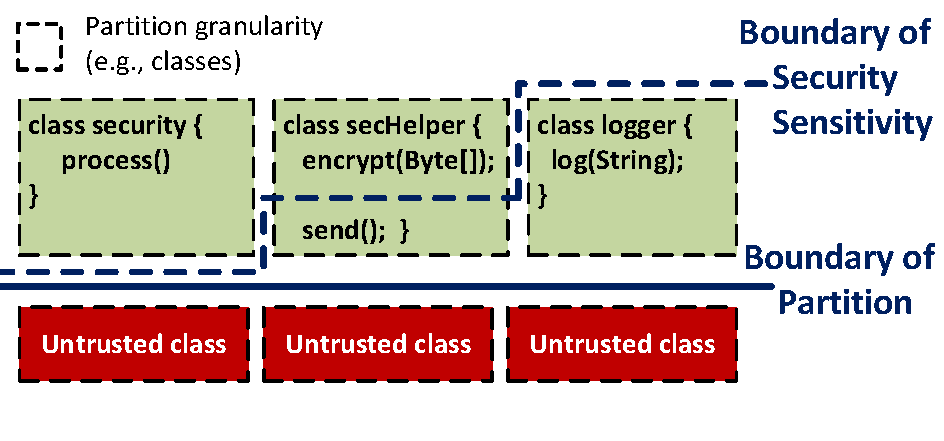
\includegraphics[width=\linewidth]{figures/partition.pdf}
%\footnotesize
%\vspace{-0.3in}
%\caption{
%Partitioning --- either manually or by automated tool ---
%often causes wider boundary of partition than the actual security sensitivity boundary
%due to (a) design granularity : {\tt SecHelper} contains a {\tt send()} method that is not partitioned from the rest of the class by design.
%or (b) better performance :  the less security sensitive {\tt logger} class is kept in 
%the privileged level to service frequent method calls. \fixmebj{Initial letter of all 
%class names must be Capital.}
%}
%\label{fig:partition}
%\end{figure}

%However, even if developers partition the applications and run only
%security sensitive components in the enclave,
%the developers may still leave some code irrelevant to
%enclave secrets inside the enclave.
%The reasons of having more-than-minimal TCB in enclaves
%are often that developers have to partition code in the granularity of source files or functions,
%or developers have to import more code to limit the width of interface and
%the frequency of interaction with the untrusted code.

\paragraph{\bf Challenge I---Cleanly partitioning classes and objects (\S\ref{sec:concept:partition})}
Java encapsulates the placement of object data and code within virtual memory, which facilitates features
like inheritance and garbage collection, but complicates integration with \sgx{}.
To program for an \sgx{} enclave, the developer must understand which regions of virtual memory 
are in the enclave, and which are outside of the enclave.
Note that \sgx{} allows code in the enclave to access memory
outside of the enclave.  Thus, it is easy for a developer to inadvertently write
code that discloses a secret, say by using a library that memoizes intermediate results to the untrusted heap.
Further, when a Java class inside of an enclave inherits methods or fields
from a parent class that is placed outside of the enclave, it is easy to 
inadvertently pass sensitive inputs to a function outside of the enclave,
or update a class field outside of the enclave.

In order for programmers to be able to sensibly program for \sgx{}, they need
a model of how objects are placed inside and outside of the enclave at runtime, as well as a model
for if and when updates to objects are propagated across the enclave boundary.
%\fixmedp{please fact check this rewrite, and make sure I am on the right track}
%\fixmebj{Looks ok to me. I will let Chia-che remove the fixmes.}
%% \sgx{} enclaves isolate the trusted components from the rest of the application,
%% and makes sure that no code or data
%% is shared between the trusted and untrusted parts.
%% For languages like C, which statically define functions and variables, it is easier for developers to cleanly
%% draw the line between trusted and untrusted components.
%% However, for a managed language like \java{}, a class can be inherited by other classes,
%% or referenced as other classes's fields, so the class may belong to both
%% untrusted and trusted components.
%% As a result, developers may struggle to manually partition the \java{} classes, especially if large portions of the classes are imported from libraries and not written by themselves.

%Reasoning about where in a program to draw the line between 
%trusted and untrusted code is subtle.
%On one hand, the developer has an incentive to minimize the size of the 
%API between the enclave and untrusted code, as well as an incentive to
%minimize the total code in the enclave.  These goals can sometimes be at odds.
%Each entry and exit to an enclave has a cost roughly comparable to a
%process context switch\fixmedp{right?}; an easy way to reduce enclave entries and exits is to simply 
%pull more code into the enclave, which increases the size of the TCB. For instance, in Figure~\ref{fig:partition}, even if the class {\tt Logger} is not security sensitive, 
%it is included in the enclave side of boundary of partition to avoid frequent entries and exits out of enclave.


%\fixmedp{I'm not sure how to explain Figure~\ref{fig:partition}, but it needs an explanation.}

%Fundamentally, the art of paritioning an application is to find a ``pinch point'' or
%``narrow waist'' in the application, where there is a natural point to insert an API and 
%security checks.  This is indeed as much art as science, often done manually by experts\fixmedp{any more supporting evidence or cites?}. Moreover, different classes of applications in managed languages like \java{} are tightly coupled; and it is necessary  to widen the boundary of partition to include some non-sensitive code in the trusted component.
%For instance, in Figure~\ref{fig:partition}, even if the {\tt send()} method is not security sensitive, it has to be included in the enclave code because of the design of the class {\tt SecHelper} to achieve a clean partition of the application.
%It is unlikely that the average developer will successfully navigate this design process without analysis tools, such as \fixmedp{examples?},
%to help identify these natural division points.


%% Experts can use a manual partitioning technique to achieve smallest TCB for the isolated components compared to automated tools.
%% However, the manual partitioning costs a lot of effort,
%% and rare expertise, lack of which can cause larger TCB.

%% Neither manual nor automated partitioning is perfect:
%% the resulted boundary of partitioning often has a gap from the actual boundary of security sensitivity (as shown in figure~\ref{fig:partition}),
%% leaving more code in the privileged level
%% than what's actually needed.
%% Having the gap between the ideal and resulted boundary
%% is mostly inevitable, due to multiple reasons.
%% One common reason is the granularity of partitioning,
%% which can vary from a binary file, a component, a source file,
%% a class, a method (a function) to a line of code.
%% Another reason is that a component or a method may be too frequently called
%% by the security sensitive code,
%% laying the boundary between the component or method from the security sensitive side may bring too much overhead or risk,
%% because the execution crosses the boundary too often.
%% Therefore, developers often will balance among the effort of partitioning,
%% risk or cost of communicating between different partitions,
%% and minimizing the TCB in the security sensitive parts.

%\fixmedp{Maybe move the commented paragraph below down into the design section?  I'd like to downplay the plugs for our work here, and instead fulfill these promises later}
%% \sysname{} automates partitioning of applications,
%% based on the boundary at the classes which the developers marked
%% as the interfaces of the enclave.
%% Only the classes that are depended by the marked classes
%% will be included in the enclaves,
%% to minimize the TCB.
%% Although not all classes pulled into the enclaves
%% are necessarily security sensitive,
%% the enclaves are protected from the potential vulnerabilities in those classes,
%% by the security guarantees of \java{} language,
%% and the information flow tracking in \sysname{}.

%Another threat to \sgx{} is the vulnerability of the 
%security sensitive code running in the Enclave. The 
%main guarantee of \sgx{} to isolate the secure data 
%from other components and privileged OS is undermined 
%if the Enclave code can be tricked to leak the 
%security sensitive data to the attacker. Executing 
%buggy code in \sgx{} enclave can inadvertently leak 
%information if the attacker can exploit memory-safety 
%vulnerabilities like buffer overflow and dangling 
%pointers.  

% Cumbersome and approximation to partition code
%The developers have to manually partition their code 
%into security sensitive and insensitive part. If this 
%partitioning is done by a novice developer, some of 
%the security insensitive parts of the application can 
%end up in the security sensitive part, increasing the 
%Trusted Computing Base(TCB). Moreover, the 
%partitioning of code is not straightforward, which 
%can also contribute to a less stricter TCB. The bigger the TCB, the more %vulnerable is the Enclave code to attacks.

% Buggy Code leads to inadvertant information leakage


% \sgx{} code only Integrity protected not confidential
%Moreover, \sgx{} only protects the integrity of the enclave code. The security critical part of the application is stored in plaintext while the secret data is provisioned securely after attestation. However, \sgx{} does not protect the confidentiality of enclave application code which may be executing a secret algorithm. \fixmebj{Talk more about the problem motivating security tag preservation.}
%\sgx{} can natively guarantee either code integrity or
%code confidentiality (as part of the enclave data), but not both.
%If application code is included in the enclave measurement and
%verified by the hardware,
%the code must stay in plaintext as part of the enclave image.
%If any code is stored or provisioned in encrypted forms,
%the application or infrastructure in enclave must dynamically load
%the code after decryption.
%Supporting dynamic loading makes enclaves open to code injection
%if the applications have exploitable vulnerabilities.

\paragraph{\bf Challenge II---Dynamically loading byte-code with integrity (\S\ref{sec:concept:loading})}
\sgx{} establishes trust by verifying the integrity of the code in the enclave.
Therefore, enclaves must be bootstrapped with static, native binaries.
%that have consistent measurements.
However, \java{} classes are shipped as byte-code,
and dynamically loaded by \jvm{}s.
The subtle security challenge for a Java developer 
is ensuring that, when a class is dynamically loaded into an enclave, by passing a string name of the class,
the application needs to be able to verify that this is a trusted class file
and that the initial state of the class is correct.
Thus, we introduce techniques to manage trust and verify the integrity of 
dynamically loaded code, including encrypted class files.

We note that using byte code is both a liability and opportunity.
One could pre-compile byte code to native code on a trusted host, and simply run the signed native code.
However, this foregoes the opportunity for performance-critical enhancements
such as profile-guided optimization or heap management optimizations for
smaller heaps.  Version 1 of \sgx{} only has up to 128 MB of total enclave page cache;
Version 2 will relax this extension.  As long as \sgx{} is a moving target,
we expect there will be value in the ability to dynamically optimize the
in-enclave code for the constraints and application behavior at runtime.

%This means the \sgx{} enclaves can only guarantee the code integrity of the initially loaded infrastructure, which in turn has to
%verify the integrity of classes dynamically loaded.
%\fixmedp{Can you say a bit more about why this is hard or interesting?}

%The hardware-level \sgx{} code integrity mechanism is based on a cryptographic
%signature of a static binary in plaintext.
%If any application dynamically loads any code after the enclave's initial measurement,
%the initial application must be trusted to attest the loaded code.
%The subtle tension is that there is no way to protect the confidentiality of
%a secret algorithm, except by dynamically loading an encrypted binary.
%Dynamically loading code increases the risk of code injection attacks and other control flow compromises. The interpreted and managed languages effectively compound the
%risks by dynamically loading all the application code.

%Any application partitioning solution that protects sensitive algorithms and data
%must have a robust dynamic loader that can measure encrypted libraries or classes.
%\sysname{} includes a loader that can measure encrypted class files,
%provisioned from a trusted host.

%% \sgx{} enclaves require code integrity in the isolated applications.
%% If the code integrity is not maintained, adversaries can corrupt the enclave code to
%% force the applications to leak the information provisioned from the remote,
%% trusted hosts.
%% \sgx{} hardware only guarantees
%% the integrity of the code initially loaded into the enclaves.
%% However, if an application choose to dynamically
%% load any code after the enclave starts,
%% the application is responsible for the integrity of the code loaded.
%% The fact that dynamic loading of applications, libraries or components
%% is a feature that can potentially make enclaves vulnerable and open to code injection,
%% raises concerns against supporting managed languages in the enclaves.

%% On the other hand, code confidentiality can be a desirable feature,
%% for application developers who prefer keeping the secret sauce of their algorithms concealed.
%% To enable the feature of code confidentiality in enclaves, the protected code must be dynamically loaded into the enclave,
%% because the \sgx{} hardware only accept
%% the initial loaded code to be in plaintext.
%% \sysname{} provides both code integrity and confidentiality by verifying
%% every classes dynamically loaded into the enclaves,
%% and allows loading classes provisioned from trusted hosts.


%% In general \sgx{} enclaves are prone to having side channels, such as timing channels. Because \sgx{} relies on the untrusted OS for paging,
%% an enclave will always leak page fault addresses, except the lower 12 bits (offsets in pages).
%% Such a leakage gives the untrusted OS to amplify the side channels,
%% by forcing page faults on every instruction or memory access.
%% This so-called {\em Controlled Channel Attack} is common to all applications who use \sgx{} protection, regardless of the programming models.
%% \sysname{} does not specifically defend against side channel attacks.

%% \paragraph{Denial-Of-Service Attacks}
%% \sgx{} is not designed to be safe against denial-of-service attacks.
%% Because the untrusted OS still controls the host resources,
%% there are countless ways to prevent an enclave from making progress.
%% For example, the OS can simply starve the enclaves by
%% never scheduling CPU, memory or other resources to the enclaves.
%% \sysname{} does not specifically defend against denial-of-service attacks.

\paragraph{\bf Challenge III---Seamless access of in-enclave objects (\S\ref{sec:concept:accessing})}
Java code outside of the enclave must be able to call enclave entry points and 
have some notion of objects that are inside the enclave.
Unlike C, where most function addresses are determined once
at the dynamic linking phase,  Java identifies most functions through
object references (e.g., {\tt Foo.toString()}).
Thus, the untrusted code must be able to reference
objects inside of the enclave in a way that makes sense when
the untrusted code behaves correctly, but that does not create unexpected information flows 
out of the enclave.
Similarly, the developer needs a constructor interface to declare which dynamically-created
objects should be placed in the enclave and which should be outside of the enclave. 


%% For native binaries, enclave entry points are statically inserted
%% into the untrusted code
%% at explicit locations known to interact with the enclaves.
%% However, for \java{} applications, instantiating or calling methods
%% on isolated components must dynamically trigger enclave entry.
%% For instance, calling the {\tt toString()} method of any object 
%% may trigger enclave entry based on whether the object's reference type is in the enclave.
%% Moreover, the the objects and methods determine the entry targets (the locations where the execution transfer after entering the enclaves) and the arguments passed into the enclaves at entry.
%% Unlike native binaries, the code behavior at enclave entry must be determined at runtime.
%% \fixmedp{I don't understand this point yet.  Is the issue that the untrusted code needs to track
%% opaque references into the enclave?  Can you explain more?}


%The \sgx{} hardware ensures that the enclave only has fixed number of entry points 
%(exactly one location where the execution starts, but multiple pre-defined locations 
%that the execution can jump to). However, for an application written in a language like JAVA with a virtual machine or interpreter, there are no clear entry points separating 
%the trusted and untrusted components. Moreover, due to the approach of executing intermediate code, it is also difficult to determine the entry points at runtime.

%Just separating an application into parts based on security sensitiveness is not enough to securely isolate the two parts using \sgx{}. In addition to application partition, there is a need to automatically determine the entry points without offloading the effort to the developers. \sysname{}  automatically identifies and exports all untrusted interfaces to the isolated classes at build time.

%\paragraph{Discussion.}
%This section has outlined several pitfalls for developers of partitioned applications.
%These common pitfalls render the hardware protections of \sgx{} useless.
%Language-level analysis can automate error-prone reasoning in the best case, or, in the worst case, 
%can at least offer invaluable guidance to the developer.  For \sgx{}-style
%hardware to be useful to a wide array of developers, developers need language-level
%tools that can also factor in hardware-level protection mechanisms.

\begin{comment}

\papersubsection{The Challenges of Combining Language and Hardware Protections}

Language and hardware protections provide varying benefits
to application security:
Languages improve the internal security inside the applications,
while hardware provides the base defenses that cannot be easily overridden or bypassed.
Commonly security experts exploits both types of protections
to further harden the security of applications.
For example, hardware protections may take information from the language runtimes or compilers to enforce the security policies,
or language protections may rely on hardware protections to bootstrap the initial trust they need. 

However, the combination of language and hardware protections is more
like a trick of the trade for security experts:
the use of hardware protections is deeply buried in the design of language protections,
so that users (application developers) lose direct access
to the security guarantees and features provided by the hardware.
\fixmets{Think of an example: Maybe TPM.}
The approaches of combining language and hardware protections are mostly ad-hoc to the use cases,
i.e., how one protection is used to improve or reinforce another.

There are two reasons for why combining language and hardware protections
is so inevitably hard.
First, hardware protections often have restrictions
on the languages that must be used
to access the security guarantees and features of the hardware.
For example, \sgx{} requires the loaded code to be implemented in C or C++,
or any languages that can compile applications into static binaries.
The restriction is not simply a design decision
made by the hardware or its SDK,
but a result of the fact that \sgx{} requires a static image to guarantee the integrity of execution.
On the other hand, if the language used is a managed language like \java{},
accessing \sgx{} hardware will be cumbersome,
because it is hard to provide any APIs to allow direct access to the \sgx{} hardware,
to harvest its security guarantees
or to utilize its features.

\begin{figure}[t!]
\centering
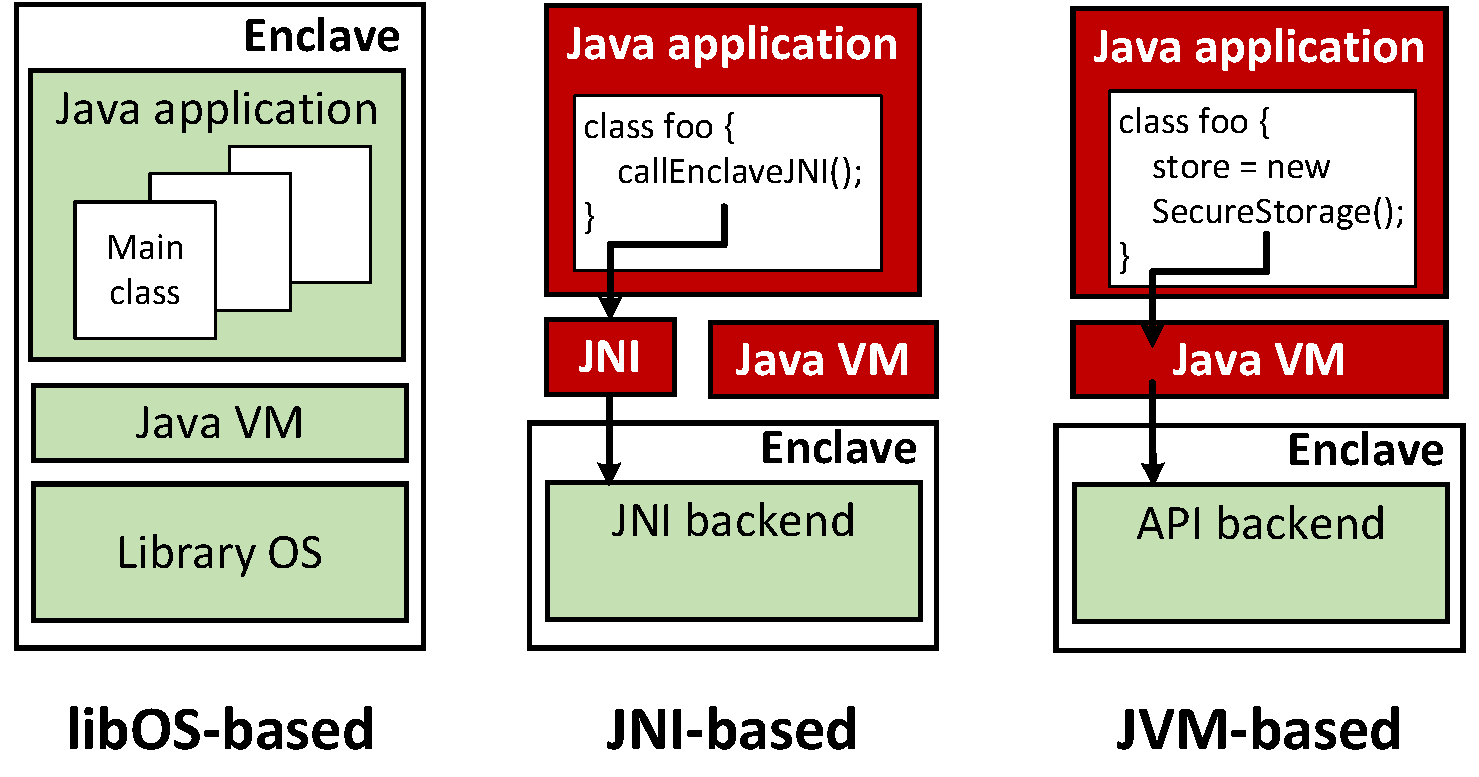
\includegraphics[width=\linewidth]{figures/alternatives.pdf}
\footnotesize
\caption{Alternative approaches to access \sgx{} hardware protection from \java{} applications.
The {\em \libos{}-based} approach runs the whole \java{} applications in the enclaves. 
The {\em JNI-based} approach uses JNI to run the security sensitive operations inside the enclaves.
The {\em \jvm{}-based} approach requires the \jvm{} to provide APIs to support common use cases of the enclaves.
Green (light) boxes are trusted components and red (dark) boxes are untrusted.
}
\label{fig:alternatives}
\end{figure}


Figure~\ref{fig:alternatives} illustrates the alternative approaches
to access \sgx{} hardware from \java{} applications:
The first approach is to run the whole \java{} applications with the \jvm{} inside the enclaves,
using a \libos{} ({\em \libos{}-based}).
This approach can secure applications as a whole,
but won't support any partitioned model for programming.
Another approach is to implement a JNI that create and interface with the enclaves
to run the security-sensitive operations ({\em JNI-based}).
The JNI-based approach is flexible enough for application developers
to implement the isolated components as well as the untrusted interface,
but requires developers to have the knowledge of
enclave implementation.
More importantly, the isolated components can only be developed in C or C++
language, so the applications lose the language protection of \java{} inside the enclaves.
A more plausible approach is to provide enclave-backed APIs
from the \jvm{},
to support common use cases ({\em \jvm{}-based})), such as a secure key-value store~\cite{vc3}.
Although the \jvm{}-based approach can save the application developers' effort
of implementing isolated components,
the use cases is limited to the pre-defined operations provided by the \jvm{} or the companion frameworks.
Because the backend implementation (isolated components and untrusted interfaces) in the \jvm{}-based approach is the same as the JNI-based approach,
the same language restriction also applies here. 

\end{comment}

%- Motivate the problem.
%- List all attack vectors
%- How can JAVA help?

\paragraph{Discussion}
Partitioning an application requires some input from the developer in order to identify 
sensitive data and code.  Each of the challenges above highlight cases where
Java either hides important information from the developer, or otherwise useful runtime
techniques can thwart the isolation benefits of using a hardware mechanism like \sgx{}.
A higher-level goal of \sysname{} is to provide constructs for the developer to specify
her goals, such as which objects should be isolated in an enclave,
and to have the language runtime use these developer-provided hints to 
make judicious choices on issues such as data placement.
A related goal is not eroding the benefits of developing in a high-level, managed language runtime.


%% The combination of language and hardware protections
%% is a technique used by many previous works.
%% However, the approach often seems like a trick of the trade for security experts:
%% the use of hardware protections is often deeply buried in the design of language protections,
%% as the underlying mechanism to bootstrap the trust
%% or to secure the core components of language protections.
%% %so that users (application developers) lose direct access
%% %to the security guarantees and features provided by the hardware.
%% %\fixmets{Think of an example: Maybe TPM.}
%% %The approaches of combining language and hardware protections are mostly ad-hoc to the use cases,
%% %i.e., how one protection is used to improve or reinforce another.
%% This work chooses a different approach,
%% by allowing \java{} applications
%% to straightforwardly utilize the protection of \sgx{} enclaves,
%% while still benefit from the safety properties
%% and advanced language protections from \java{}.
%% As a result, our framework also opens the win-win opportunity for
%% hardening both \sgx{} and \java{} protections.
%% \fixmedp{I also don't understand the point of this discussion.  What do you want the reader to learn from this?}

%\papersection{Threat Model}
\label{sec:threat}

In this section, we discuss the threat model of \sysname{},
including the adversaries,
and the components that must be trusted.

\paragraph{Adversaries}
We assume the same adversaries as other \sgx{} enclaves.
Any part of the system stacks, including the OSes,
device drivers, hypervisors, and even hardware,
such DRAM, GPU, buses, and peripheral devices, can be malicious
and attempt to attack the enclaves.
%The only trusted component is the CPU package, including L2 and L3 caches.
The attackers can perform any form of
online and offline attacks.
We also assume the attackers own all information
about \sgx{} hardware implementation, as well as every part of our solution.

We focus on the adversaries that target on
exploiting vulnerabilities in the isolated applications.
The attackers can manipulate any input to the application interfaces,
or the untrusted interfaces of the enclaves.
%Attackers may apply any techniques that compromise a regular privileged applications to compromise enclaves.
The vulnerabilities that attackers can exploit may not only fall in applications, but also in the infrastructures,
such as the libOS, the \java{} VM, JNIs and low-level interface to architecture.

%The only adversaries that are not addressed in \sysname{} are
%attackers exploiting {\em side channels} and
%{\em denial-of-service attacks}.
%Side channels, or even controlled channels, is a known problem of \sgx{} enclave
%and we expect to solve the problem in the future with
%stronger architectural support.
%Denial-of-service attacks are often considered benign for enclaves,
%because it only affect the ability of an untrusted host to legally access
%critical resources.

\paragraph{Trusted Components}
We trust any components loaded inside an enclave,
including the infrastructure (details discussed in Section~\ref{sec:implementation}), %(low-level interface, the libOS, \jvmname{}),
all supporting classes and their JNI,
and other resources or classes provisioned from remote hosts.
%All trusted components must be verified by either \sgx{} hardware or the infrastructure against their cryptographical measurements or checksums.
The implementation of \sgx{} hardware is also trusted to be invulnerable,
and use adversary-resistant key generators that cannot be compromised
by online or offline techniques.
We also assume \intel{} CPUs are resistant to direct, physical attack to the CPU packages, either to modify or peek into the chips.

\fixmets{Now JIT'ed code is not giving me error, but in case it fails later, we have to flip this discussion.}
We support running \java{} application both with and without JIT optimization.
Running \java{} application with JIT optimization
improve the performance of execution,
but can cause massive increase of the TCB of enclaves.
In case that JIT optimization is enabled in the enclaves,
the JIT compilers (\java{} VMs often have multiple JIT compilers, e.g., \jvmname{} has two) must be trusted by the users,
to always generate correct and invulnerable binary code.


%Note that in \sysname{} we disable JIT compiler that used to improve \java{} execution performance.
%The choice of disabling runtime compilation is due to the concerns that
%JIT compiler may largely extend the TCB because it must be trusted,
%and any bugs in different versions of compilers
%may causes code behaviors than what developers have tested and expect.
%Another practical reason is concerning the complexity and
%resources required for running a \java{} compiler with library OS in an %enclave.
%However, we consider these limitations to be not fundamental to the approach, and we keep compiler support in \sysname{} as a future work.



%In term of architecture, we trust the implementation of \sgx{} hardware,
%to maintain invulnerable implementation of \sgx{} instructions,
%and using adversary-resistant key generators that cannot be compromised
%by attacker using online or offline techniques.
%The CPU must keep enclave contents encrypted in DRAM and low-level caches that are shared by multiple cores.
%We also assume \intel{} CPUs are resistant to direct, physical attack to the CPU packages, either to modify or peek into the packages.

%\sysname{} protects confidentiality and integrity of provisioned security critical data in the trusted part of an application written in a high level managed language like JAVA.
% from the privileged operating system and the untrusted part of the same application. 
%\sysname{} assumes that the \sgx{} instructions are implemented correctly in the processor, and the SDK do not contain exploitable bugs to leak information. In addition, \sysname{} trusts the Graphene LibOS and the JVM running in the enclave with the trusted part of the application to not leak information. Thus, the security of the provisioned data is limited by the correctness of the processor, \sgx{}, Graphene LibOS, and JVM. \sysname{} also trusts the trusted part of the application to not leak information explicitly. \sysname{} prevents the trusted part of an application from implicitly leaking information.

%Threats that we do not cover
%\sysname{} inherits the threat model of \sgx{}~\cite{sgx}.
%The adversary controls the cloud provider's complete stack, OS, hypervisor, BIOS, system management mode, platform firmware, and device firmware. The adversary can also probe the memory and manipulate the I/O, but cannot read secret present in the processor.
%\sysname{} do not defend against attack vectors such as side-channel, covert-channel and control-channel~\cite{control-channel}. Denial of Service (DOS) attack is not part of \sysname's threat model. Even if the OS never schedules the enclave program or the untrusted part of the application is manipulated to never enter the enclave, no provisioned secret is leaked outside the enclave.


\chapter{System Overview}
\label{chap:overview}

\makeatletter
\def\input@path{{overview/}}
\makeatother
\graphicspath{{overview/figures/}}

%\section{Introduction}
%\label{sec:dcache:introduction}

Operating System kernels commonly cache file system data and metadata in 
a virtual file system (VFS) layer, which abstracts low-level file systems into a common API, 
such as POSIX.  
This caching layer has become a ubiquitous optimization
to hide access latency for 
persistent storage technologies, such as a local disk.
%whether a local disk or a network appliance, 
%have substantially higher access latencies than RAM,
%this caching layer 
%% SOSP Space - kind of quacking on
%% Caching
%% the file system directory hierarchy is particularly important because 
%% low-level file systems often spread this information across 
%% multiple disk sectors.
%% If an application wanted to open a single file on a system without a directory cache, 
%% most low-level file systems would issue numerous disk reads to locate the file and check the permissions
%% on the file and its parent directories;
%% a directory cache can commonly avoid these reads.
The directory cache is not exclusively a performance optimization; it also simplifies 
the implementation of {\tt mount}-ing multiple file systems, 
consistent file handle behavior,
and advanced security 
models, such as SELinux~\citep{selinux}.



%\fixmedp{Be charitable to developers, make our strong claims positively (we are really smarties) rather than calling them dummies}


%% Many observation shows that, in most systems, operations to storage are often
%% dominated by hierarchical structure traversal,
%% and fetching metadata of objects.\fixmetsai{references here}~\citep{duchamp94nfs}
%% In many file systems, traversal and metadata fetching
%% create random access patterns,
%% which are slower than sequential access patterns
%% on many storage media, e.g. magnetic disks.

% dp: I think this is getting down in the weeds.  We need to make the case for the work 
%     more strongly and generally first
%% Directory entry cache, a.k.a \dcache{},
%% is an important optimization in Linux kernels
%% to reduce storage operations for traversal and metadata fetching.
%% The design of \dcache{} is comparable to \vnode{} in BSD and \dnlc{} in Solaris.
%% \dcache{}, as well as \vnode{} and \dnlc{},
%% can be explained as a file system layer that
%% responds to requests on a cache hit,
%% but passes requests down to lower-leveled file systems on a cache miss~\citep{zadok06, skinner93}.

%\fixmedp{F1: Maybe thread together an argument about why no one would have tried a one-hop lookup before?}


%\marginpar{\scriptsize \textcolor{blue}{ Michael, I think the high-order bits are mostly right on Fig~\ref{fig:dcache:lookup-frac},
%but these number may change a bit as we refine the measurement}}

\begin{figure}[t]
\scriptsize
\centering
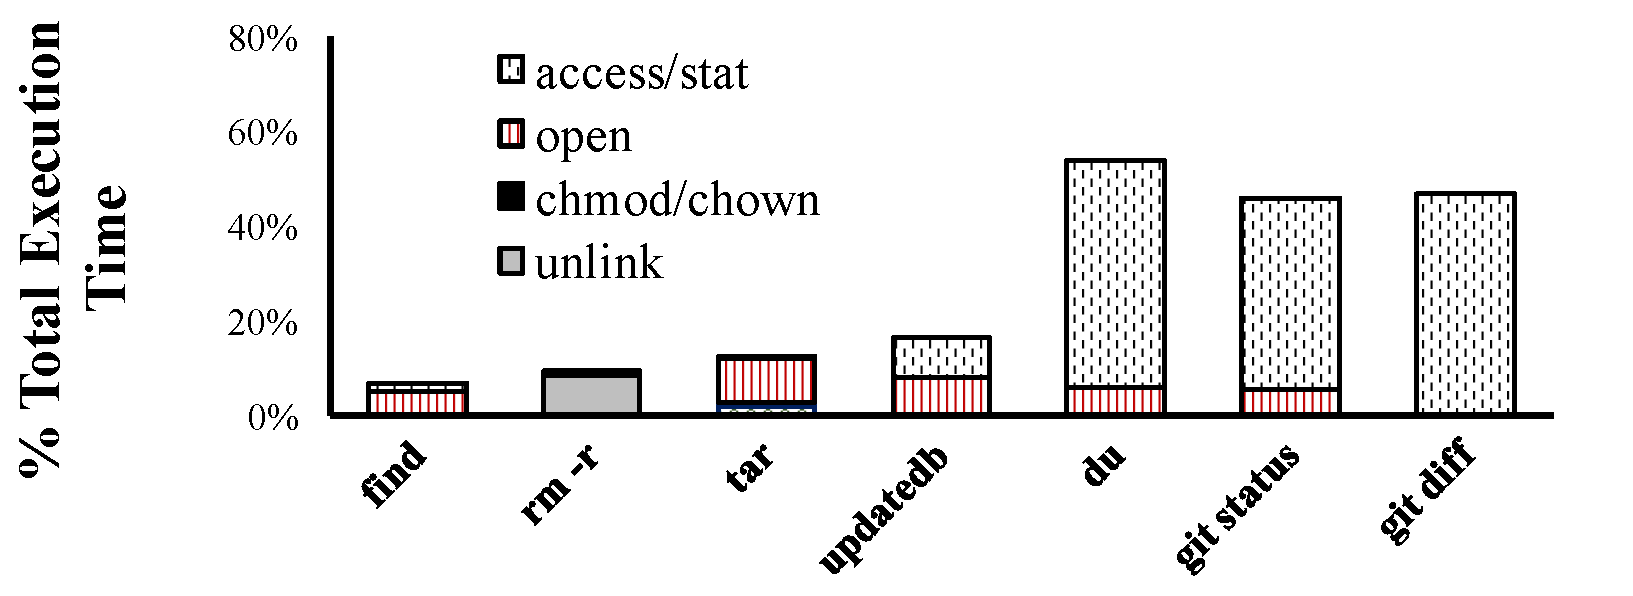
\includegraphics[width=5in]{dcache/plots/syscall-percentage.pdf} \\
\caption[Fraction of execution time on path-based system calls.]
{Fraction of execution time in several common utilities spent
executing path-based system calls with a warm cache, as measured with ftrace.}
\label{fig:dcache:lookup-frac}
%\vspace{-10pt}
\end{figure}

%\fixmedp{Please check these \% against time.  I think git diff is too high.  git status seems ok.}

Directory caches are essential for good application performance.
%Unix was designed such that ``(almost) everything is a file'',
%thus even accesses to in-memory file systems, device files, FIFOs and domain sockets
%first pass through the directory cache.
%In other words, 
Many common system calls must operate on file paths,
which require a directory cache lookup.
For instance, between 10--20\% of all system calls in the iBench system call traces do a path lookup~\citep{filenotafile}. 
Figure~\ref{fig:dcache:lookup-frac} lists the fraction of total execution time
%, as well as system time, 
several common command-line applications spend executing path-based system calls
(more details on these applications and the test machine in \S\ref{sec:dcache:eval}).
We note that these system calls include work other than path lookup,
and that these numbers include some instrumentation overhead;
% are coarse measurements that include  and work than path lookup;
%, and includes some time 
%for synchronous I/O (e.g., during {\tt rename}) as well as non-path tasks (e.g., creating 
%a file handle as part of {\tt open});
nonetheless, in all cases except {\tt rm},
the system call times and counts are dominated by
{\tt stat} and {\tt open}, for which 
%can be serviced from cache and for which 
path lookup is a significant component of execution time.
For these applications, path-based system calls account for 6--54\% of total execution time.
%and 25--77\% of system time.  
This implies that
lowering path lookup latency is
 one of the  biggest 
opportunities for a kernel to improve these applications' execution time.




\begin{figure}[t!]
\centering
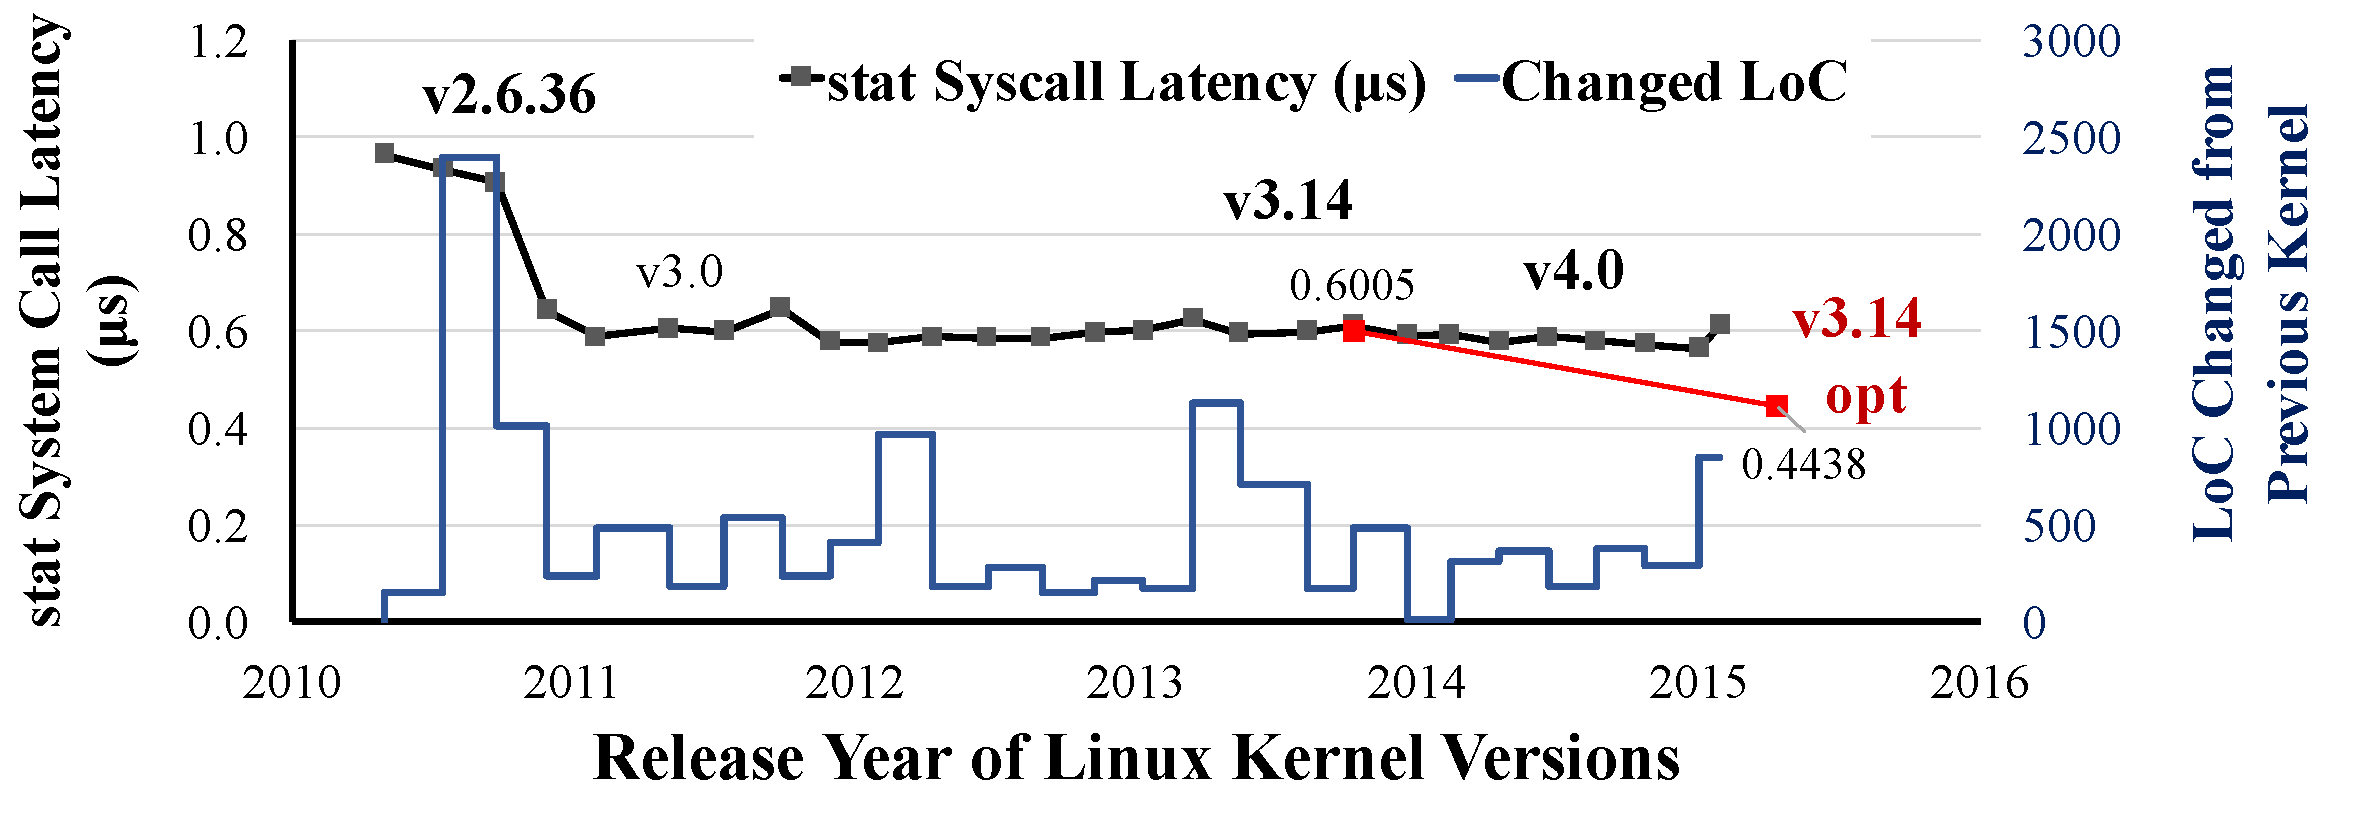
\includegraphics[width=6in]{dcache/plots/latency-by-version.pdf}
\footnotesize
\caption[Lantecy of {\tt stat} system call over years.]
{Latency of {\tt stat} system call with a long path {\tt XXX/YYY/ZZZ/AAA/BBB/CCC/DDD/FFF} on Linux over four years (lower is better), as well as the churn within the directory cache code (all insertions in {\tt dcache.c}, {\tt dcache.h}, {\tt namei.c}, {\tt namei.h} and {\tt namespace.c}). 
%Our optimizations significantly improve performance that has otherwise plateaued, despite significant ongoing developer effort.  
Our optimized \linuxver{} kernel 
further reduces {\tt stat} system call latency by \statspeedup{}\%.}
%\vspace{-15pt}
\label{fig:dcache:by-version}
\end{figure}


%\fixmedp{Add more evidence of lookup importance here: For instance, fraction of lookup time in file-related syscalls, or total lookup time in applications bound on file lookup latency.  }
Unfortunately, even directory cache hits are costly---0.3--1.1 \us{} for a {\tt stat} on our test Linux system, compared to only .04 $\mu$s for a {\tt getppid} and 0.3 \us{} for a 4 KB {\tt pread}. 
%\fixmetsai{Don, check this, I think read will be a better example, getppid is too trivial.}
This issue is taken particularly seriously in the Linux kernel community, which has 
made substantial revisions and increasingly elaborate optimizations to reduce the hit cost
of its directory cache, such as removing locks from the read path or replacing lock ordering with deadlock avoidance in a retry loop~\citep{corbet09jls,dcache-rcu}.
Figure~\ref{fig:dcache:by-version} plots directory cache hit latency against  lines of directory cache code changed 
over several versions of Linux, using a path-to-inode lookup \microbench{} on the test system described
in \S~\ref{sec:dcache:eval}.
These efforts have improved hit latency by 47\% from 2011 to 2013, but have plateaued
for the last three years.
%\fixmedp{if time, filter irrelevant changes from code deltas}
%at the cost of substantial developer effort.
%This latency appears to have plateaued 

The root of the problem is that the POSIX path permission semantics
seemingly require work that is linear in the number of path components,
and severely limit the kernel developer's implementation options.
%The root of this problem is that current directory cache
%designs reflect a straightforward implementation of the POSIX specification,
%which would seemingly require work that is linear in the number of path components.
For instance, in order to open file {\tt /\fnone{}/\fntwo{}/\fnthree{}} 
%for reading, 
one must have search permission
to parent directories {\tt /}, {\tt /\fnone{}}, and {\tt /\fnone{}/\fntwo{}},
as well as permission to access file {\tt \fnthree{}}.
The Linux implementation %of this specification is straightforward, 
simply walks the directory
tree top-down to check permissions.  
Unfortunately, when the critical path is dominated by 
walking a pointer-based data structure, 
including memory barriers on some architectures for multi-core consistency, 
modern CPUs end up stalling on hard-to-prefetch loads.
Moreover, because so many Linux features are built around this behavior, such as Linux Security Modules (LSMs)~\citep{wright+lsm},
namespaces, and mount aliases, it is not clear that any data-structural enhancements
are possible without breaking backward-compatibility with other Linux kernel features.
A priori, it is not obvious that a faster lookup algorithm, such as a single hash table lookup, 
can meet these API specifications and kernel-internal requirements; to our knowledge,
no one has tried previously.

%This paper proposes a decomposition of the directory cache, which allows
%most lookup operations to execute with a single hash table lookup (\S\ref{sec:dcache:dcache}),
%as well as optimizations to reduce the miss rate based on information that is {\em already in the cache}, but not used effectively (\S\ref{sec:dcache:readdir}).
%Our design maintains compatibility (\S\ref{sec:dcache:generalize}) through 
%several essential insights, including 
%how to separate the indexing of paths from checking parent permissions,
%and how to effectively and safely memoize the results of access control checks.


%% This paper proposes several new ways to organize a directory cache, which can yield 
%% substantial performance improvements over the current state of the art.
%% %This paper demonstrates that, despite this developer effort, there is still a substantial 
%% %missed opportunity hiding behind historical, intuitive, but not fundamental design choices.
%% Most of the Linux directory cache design reflects a straightforward implementation of the POSIX 
%% specification. %, with a division of labor that is suitable for mainstream file systems.

%This paper presents an alternative directory cache organization, which 
%improves performance by separating logical tasks, such as separating path indexing from permission checking; yet the design is sufficient to retain compatibility with POSIX.
%In the case of path lookup, 
%this paper demonstrates how 
%a per-component tree walk can be replaced with a single hash table lookup (\S\ref{sec:dcache:dcache}).
% without violating POSIX compliance.

%Our optimizations improve the performance of frequent lookup operations, but 
%introduce several costs, described in \S\ref{sec:dcache:dcache} and measured in \S\ref{sec:dcache:eval},
%which  we believe are acceptable and a net improvement for applications.
%First, these optimizations slow down infrequent modifications to the directory hierarchy, such as {\tt rename}, {\tt chmod},
% and {\tt chown} of a directory. 
%However, these slower operations
%account for less than .01\% of the system calls in the iBench traces~\citep{filenotafile}.
%Second,  the memory overheads of the dcache are increased.
%%(45\% per \dentry{}, as well as some  in our prototype).
%%(\fixmedp{XX MB} in our tests).  
%Third, lookup has a 
%probability of error from signature collisions that can be adjusted to be negligible
%%($2^{-141}$ in our configuration), 
%and within acceptable thresholds widely used by data deduplication systems~\citep{Debnath:2010:CSU:1855840.1855856, Srinivasan:2012:ILI:2208461.2208485, Quinlan:2002:VNA:645371.651321, Zhu:2008:ADB:1364813.1364831}.
%%, as well as how to remove
%%all memory barriers from the lookup path (\S\ref{sec:dcache:update}).
%In the micro-benchmark of Figure~\ref{fig:dcache:by-version}, our directory cache 
%optimizations improve lookup latency by 
%%revisions improve latency of accessing a long path
%%by 
%\statspeedup{}\% over unmodified Linux.
%%Our design addresses other missed
%%opportunities, such as identifying new opportunities to reduce the miss rate
%%through caching directory completeness.
%%\fixmedp{Do we want to highlight LoC?  3K is more than anything in the graph} \fixmetsai{Probably just mention in the evaluation. It's a metric that we should provide, but it's not awfully interesting.}
%%The total lines of code changed are fewer than 3,000 out of \fixmedp{XX}.
%%\fixmedp{Can we get 
%%, yet changes fewer than 3,000 lines of code.

%% SOSP cut - kind of long-winded
\begin{comment}
This paper rethinks current Linux directory cache design choices in light of the following goals:
\begin{compactitem}
\item {\bf Minimize the cost of a cache hit.} (\S\ref{sec:dcache:dcache}).
This means maximizing the benefit of temporal locality for frequent operations,
while pushing extra work of consistency maintenance onto less frequent, already-expensive operations.
%such as handling cache miss or updating massive metadata,
%in order to improve very frequent operations.
\item {\bf Maintain legacy compatibility.} (\S\ref{sec:dcache:generalize}).  Unix path semantics are complex, required by applications, file systems, and security modules, frustrating otherwise straightforward optimizations.  However tempting it may be to redesign path behavior to facilitate caching, path operations must exhibit the same behavior, with lower latency.
\item {\bf Never miss the same request twice in quick succession.} (\S\ref{sec:dcache:readdir}).  A number of less-frequent operations, such as reading a directory or secure temporary file creation, always miss in the cache {\em even if enough information is in cache to satisfy the operation.}  
%Of course, infrequent accesses should still be subject to a cache replacement policy, such as LRU.
\end{compactitem}
%Although directory caches must implement more complex semantics than a hardware memory cache,
%these principles should seem familiar to the reader with a basic architecture background.
%sadly, the Linux directory cache design violates all three.
\end{comment}

%This paper introduces several techniques to improve the performance of a directory cache,
%This paper explains several practical directory cache optimizations,
This paper demonstrates that these techniques improve performance for applications that use the directory cache heavily,
and the harm is minimal to applications that do not benefit.
%and that the worst case \microbench{} is only 12\% slower within \fixmedp{XX}\% of unmodified Linux.
%Each optimization we describe improves performance in isolation, and all can be combined.
%These optimizations change very few lines of code, and are backward-compatible with 
%legacy applications.  
%These changes are encapsulated in the VFS---individual file systems do not have to change their code.
%This paper describes a  prototype of these improvements implemented in Linux \linuxver{}.
%\S~\ref{sec:dcache:background} explains that the directory cache structure of Mac OS X, FreeBSD, and Solaris 
%are sufficiently similar that these principles should generalize.
%we compare and contrast Linux's directory cache
%with Mac OS X, FreeBSD, and Solaris in \S\ref{sec:dcache:background}, and explain inline how each
%optimization could be generalized to these other OS kernels.





%% \item {\bf Modularization and stackability}:
%% Any changes or optimizations must be implemented as modules inside Linux's VFS,
%% and can be stacked on top of the original design or any future optimizations. 
%% \item {\bf Backward compatibility}:
%% Any changes or optimizations must maintain least requirement of modifying any
%% file systems.
%% \item {\bf Generalization to other OSes}: Any changes or optimizations must be portable to other OSes with reasonable effort and change of design.




%% \dcache{} is proven to be effective on improving storage performance.
%% Experiments shows that,
%% in a Linux 3.x kernel, a \dcache{} with a xxx\% hit rate can speed up
%% metadata lookup and fetching time by xxx times.
%% \fixmetsai{experiment result, Linux version, and fs specs here}
%% However, we observed that Linux maintainers have made
%% constant and non-trivial efforts to improve \dcache{} in the Linux kernel.
%% We studied all \dcache{}-related source files in the Linux kernel Git repository,
%% and discovered that maintainers have committed
%% on average xxx revisions per source files.

%% We tested metadata lookup time on primary \dcache{}-related revisions.
%% Most changes on \dcache{} system only create xxx\%-xxx\% speed-up
%% than their predecessor.
%% \fixmetsai{result and graph here}.
%% Moreover, improvement to \dcache{} is still work-in-progress
%% for Linux maintainers.
%% \fixmetsai{reference to threads for latest dcache discussions}. 
%% All the evidences show that,
%% despite of significant reduction of storage operations,
%% efficiency of \dcache{} system internally still remains as a concern.

%% We argue that the design of \dcache{} needs to be carefully re-examined,
%% to fundamentally identify any missed opportunities that
%% improve value of \dcache{}.
%% At a high level, most optimization works for \dcache{} are focused on
%% improving ``how to cache'',
%% but we want to also lay eyes on ``what to cache'',
%% to ensure any valuable information returned from file systems
%% be captured by \dcache{} system.

%The contributions of this paper are as follows:
%\begin{compactitem}
%\item A performance analysis of the costs of path lookup and the opportunities
%to improve cache hit latency.
%\item A directory cache design that improves path lookup latency with a combination of techniques, including:
%  \begin{compactitem}
%  \item Indexing the directory cache by full path, reducing average-case lookup from linear to constant in the number of path components.
%  \item A Prefix Check Cache (PCC) that separates permission checking from path caching.  The PCC memoizes permission checks, and is compatible with LSMs~\citep{wright+lsm}.
%  \item Reducing the cost of checking for hash bucket collisions with path signatures.
%  \end{compactitem}
%\item Identifying opportunities to leverage metadata the kernel already has to reduce miss rates, such as tracking whether a directory is completely in cache.
%\item Carefully addressing numerous, subtle edge cases that would frustrate rote application of these techniques, such as integration with symbolic links and Linux namespaces.
%\item A thorough evaluation of these optimizations.  For instance, our optimizations improve throughput
%of the Dovecot IMAP server by up to \dovecotspeedup\% and latency of 
%updatedb by up to \updatedbspeedup{}\%.
%%git version control system by up to 25\%.
%
%\end{compactitem}

\papersection{\Thehostabi{}}
\label{sec:overview:host}

\issuedone{1.1.b}{Describe \thehostabi{} specification}
The development of \graphene{} starts with defining a simple host ABI (application binary interface) called \thehostabi{},
containing only OS abstractions essential to target applications.
%and is easily ported to different platforms.
%and minimal specifications for the host OSes and hardware.
%The host ABI is a new boundary between OSes (or hypervisors) and applications.
\Thehostabi{} separates
the implementation of an existing system API (application programming interfaces), which determines the compatibility against applications,
from hardware abstraction features, such as file systems, network stacks, and device drivers. 
\graphene{} moves the system API components
to a \libos{} in the userspace and reimplements the functionality using \thehostabi{}.
To port \graphene{} to a new host OS or hardware,
OS developers only have to implement \thehostabi{} on the target host system API,
%to new host OSes and hardware,
instead of paying a tremendous cost to translate the whole system API specification. Figure~\ref{fig:overview:porting} illustrates the porting process of \graphene{}.



%The host ABI separates the low-level, hardware management features, from the idiosyncrasy of system interface. 
%\graphene{} moves the upper layer of OS components,
%including the system calls and namespaces, into an library OS,
%leaving \thehostabi{} 
%as a narrowed interface to the host OSes and hardware.
%The host ABI intends to minimize the development effort on each host OS or hardware
%to mitigate the interface distinctions,
%to simply porting the OS abstractions defined in \thehostabi{}.


\begin{figure}[t!]
\centering
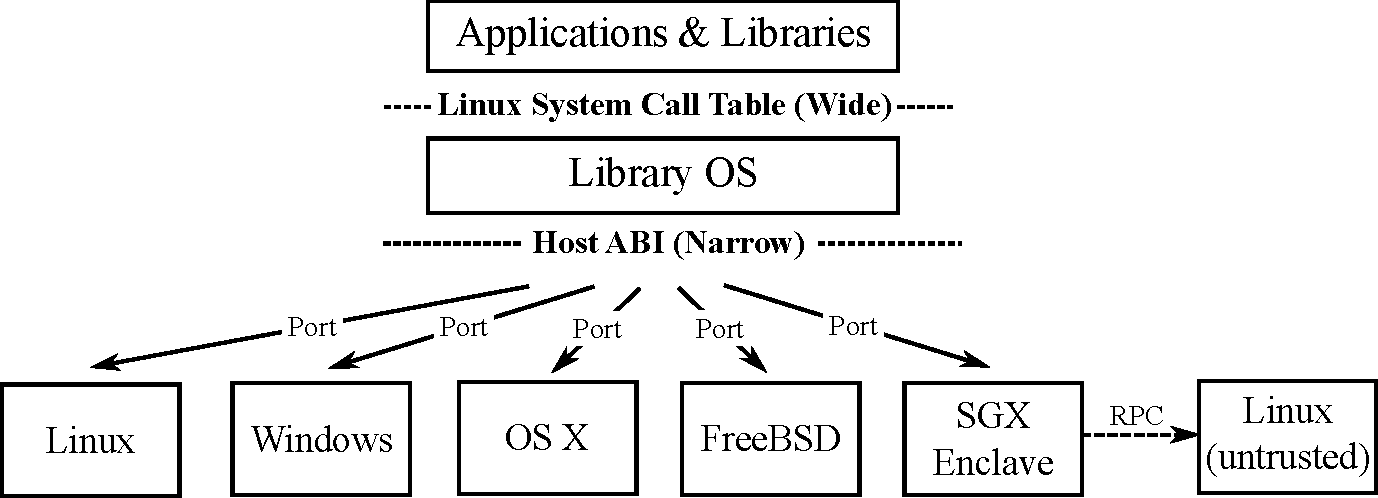
\includegraphics[width=30em]{porting.pdf}
\caption{Porting model of \graphene{}.}
%\vspace{-.1in}
\label{fig:overview:porting}
\end{figure}



\papersubsection{Platform Adaption Layers (PALs)}
\label{sec:overview:host:pal}


For each host OS or hardware, \graphene{} uses
a thin library called a {\bf platform translation layer (PAL)}
to translate among host interfaces.
%is loaded below the library OS, to translate each functions in \thehostabi{} to native system interfaces.
The main purpose of a PAL is to mitigate the semantic gap
between \thehostabi{} and
native host system APIs.
%The effort of PAL development is per host OS, whereas the library OS implementation is reusable on every hosts. %The simplicity of \thehostabi{} can be also estimated by the effort of implementing a PAL for each host.
By implementing a PAL on a new host OS or hardware,
users can reuse
the same \libos{} to run the same collection of unmodified Linux applications.
%To keep the porting effort low,
%the development of a PAL must be straightforward
%for average OS developers.
%to achieve with limited efforts.
%Based on the principle of porting simplicity, PAL development must be straightforward
%for average developers.







%The host ABI is defined for the simplicity of porting, as well as the sufficiency for implementing a library OS compatible to Linux.
%First of all, the number of host functions included in \thehostabi{}
%is much smaller than the number of system calls in a commodity OS such as Linux. 
\graphene{} currently contains PAL implementations for several popular OSes,
including Linux, \win{}, \osx{}, and FreeBSD.
%and \sgx{} with an untrusted Linux kernel.
Most of these OSes provide a POSIX-like system API similar to \thehostabi{}.
Due to the similarity, translating most of \thehostabi{} to one of the system APIs
are straightforward for average OS developers.
\Thehostabi{} is also much smaller than the actual POSIX API, making it extremely portable.



A part of \thehostabi{} may be challenging to port
on an OS,
due to unexpected system assumptions made by the OS.
For instance, \win{} does not support
fine-grained memory deallocation for de-privileged applications.
To implement system calls like \syscall{munmap} and \syscall{mprotect},
\graphene{} needs host ABIs to
deallocate or protect virtual memory pages at page granularity.
%A workaround is to change memory mappings at the physical page level,
%but will require running the \win{} PAL with root permissions.
%This type of porting challenges
%tends to be results of design decisions or assumptions made by OS developers.
%A \libos{} can potentially design
%different emulation strategies
%to compensate missing host abstractions.
A few host abstractions such as a bulk IPC feature are
optional to the host ABI;
if a host OS does not support these abstractions,
the \libos{} must fall back to alternatives. 

%In our experience, the development of a PAL is around ten thousand lines of code.

%For each port, the amount of code written for implementing \thehostabi{} is at the order of magnitude of thousands of lines of code, which is much more manageable than implementing a flat translation layer for system interfaces.


\begin{comment}
Based on the experience in \graphene{},
it is hard to ensure the portability of \thehostabi{} on every potential hosts.
%even a host ABI specialized for simplicity cannot guarantee to be portable on every hosts.
A host may simply lacks the functionality
for implementing a \hostapi{}.
The assumption is, maintaining the compatibility of \thehostabi{} poses a much less challenge than maintaining the whole system API.
Besides, the library OS may flexibly switch among emulation strategies
to compensate the absence of certain host abstraction.
As an example,
bulk IPC is optional in \thehostabi{} since its first definition,
due to the expectation
that implementing the feature may not be feasible on some hosts.
If bulk IPC is not available,
the library OS can fall back to RPC-based IPC, with a reasonable amount of performance penalty.
In the worst case, if there is no emulation strategies
to compensate for the absence of a \hostapi{},
user can predict the affected applications and avoid running these applications
on specific hosts. 
%at least users can predict whether an application will be affected and thus cannot run on certain hosts.
\end{comment}


%For a host OS that does not support ELF binaries, the PAL must follow the binary format which the host OS accepts, such as the Portable Executable (PE) format on \win{}.
%The PAL is the only layer in the user space which cannot be reused
%across different hosts. Besides the PAL, all of the other binaries in the user space are fully reusable, including the library OS, the supporting libraries, and the application executable.



%The host abstractions map to several common system calls in a commodity OS.
%For example, \funcname{StreamRead} and \funcname{StreamWrite} can directly map to the POSIX functions \funcname{pread} and \funcname{pwrite}, which are available in most OSes including Linux, BSD, \osx{}, and \win{}.
%More than half of the functions in \thehostabi{} can be counted toward this category.
%The rest of the host abstractions are either specific to Linux
%(e.g., TLS support),
%or belong to the POSIX functions that are not shared with commodity OSes
%(e.g., \funcname{mmap} on \win{}).
%The PAL emulates these host abstractions, using existing system interfaces available on the host OS, unless the software emulation is fundamentally impossible (e.g., restricted by the system interfaces), or too expensive (e.g., high overhead from copying data).



\papersubsection{Definitions and design principles}
 

\graphene{} defines \palcallnum{} calls in \thehostabi{} (also called \hostapis{}),
with a set of host abstractions
sufficient for \libos{} development.
%The host ABI defines the interaction between the library OS and a specific host.
%The \graphene{} library OS can be deployed on any ``host'' where \thehostabi{} has been ported.
This thesis defines
a {\bf host} of \thehostabi{}
to be an OS or hypervisor
which contains enough OS functionality for running a standalone application or virtual machine.
Most of the host targets in \graphene{}
are monolithic OSes,
including Linux, \win{}, \osx{}, and FreeBSD.
%which has defined a massive system API for programmability.
A monolithic OS 
usually contains a massive amount of system APIs,
which is sufficient for
implementing \thehostabi{}.


A special example of a host
is an \sgx{} (Software Guard Extensions) enclaves~\cite{intelsgx},
which
restricts OS functionality for security reasons.
The restrictions on \sgx{}
are results of a strong threat model
which distrusts any OS features except ones that are virtualized by the CPUs or migrated into enclaves.
The only way to obtain any missing OS features such as storage or networking
is to request through RPC (remote procedure call).
Requesting untrusted OS services through RPC also introduces new security threats that application developers tend not to anticipate~\cite{checkoway13iago,osdi16scone}.
Due to all the compatibility and security challenges discussed above,
this thesis uses \sgx{} as a representative example of a host
with unusual assumptions (e.g., threat models) and restrictions
compared to a monolithic OS.

%An innovative hardware abstraction like \sgx{} (software guard extensions)
%imposes unique assumptions and restrictions
%on a commodity OS,
%%creates a special host on top of Linux or \win{},
%%with unique interfaces and specifications regarding the host OSes.
%and thus creates a special host above the OS.

%If an OS has mutated or tweaked the interface for a hardware platform,
%such as an \sgx{} enclave 
%running on an untrusted Linux kernel,
%the combination of the OS (Linux) and the hardware platform (\sgx{}) is considered a specialized host.
%Especially, the \sgx{} port of \thehostabi{} faces several unique challenges,
%which will be discussed in Chapter~\ref{chap:sgx}.


\begin{comment}
%\fixme{each sentense should be a paragraph; starting the 2nd sentence}
\fixmedp{start with a strong opening stating the rationale}
The host ABI of \graphene{}
define functions needed from a host, in order to implement the library OS for reusing applications.
%to reuse an application and all its supporting libraries, including the \graphene{} library OS.
Each host of \graphene{} contains an OS and a hardware platform, either of which causes compatibility issues for running unmodified applications.
OS developers can port the library OS to a new host,
by simply reimplementing the narrowed host ABIs using abstractions available on the host.
%a new host platform.
%For each host which requires the compatibility for unmodified Linux applications, one only has to implement the narrowed host ABIs,
%instead of reimplementing the bloated, ``legacy'' system interfaces
%needed by the applications.
By implementing \thehostabi{}, OS developers skip the painful process of rebuilding the whole system interfaces of a commercial OS such as Linux.
The host ABIs strictly decouples the porting effort on the hosts from the compatibility feature for applications.
%The host ABIs decouple the OS development in the host and the implementation of compatibility for the existing Linux application.
What \thehostabi{} exposes is a simplified extended machine,
similar to a para-virtualization interface, capable of running the library OS as a lightweight virtual machine. % with compatibility against Linux applications.
%on which another layer of virtualization (i.e., the library OS) can be built to reproduce the compatibility for Linux.
\end{comment}


\begin{comment}
Two design principles drive the definition of \thehostabi{}s:
{\em simplicity} (i.e., easy to port on any hosts)
and {\em sufficiency} (i.e., containing enough OS functions for implementing a library OS).
The process of deciding \thehostabi{}s is comparable to
finding a ``pinch point'' within a OS implementation,
which can conveniently mediate a significant portion of OS execution paths for managing hardware abstractions.
%The two principles drive the development of \thehostabi{}s,
%The whole development of the \graphene{} library
%must be disciplined
%on extending \thehostabi{}s only when it is strongly required.
%of restraining extensions to \thehostabi{}s unless absolutely necessary.
The two principles
determine the soundness of the \graphene{} approach to improving compatibility
for any hosts.
\end{comment}


%%The host ABI is defined with partitioning in mind.
%\Thehostabi{} 
%determines a boundary which partitions several upper-level OS components, %, such as system calls and namespaces,
%into a library OS,
%%, as a dynamically-linked library which can be deployed
%%to various hosts.
%%The rationale behind the partitioning is based on the fact that not every OS component is equally important to compatibility, for applications which need to be ported across hosts.
%%When an OS is extended for a new hardware,
%%these OS components usually remain unchanged, or are predominantly reused.
%%Partitioning
%%into a library OS further guards these 
%in order to isolate the host idiosyncrasy. % on specific hardware. %any potential changes for adopting new hardware.
%%Similar isolation
%%exists in traditional OSes, but without partitioning:
%The strategy
%is also used in OSes:
%An example is the Linux virtual file system (VFS), an internal interface
%which encapsulates operations of file system drivers.
%%On the other hand,
%%drivers (e.g., drivers for file systems, block devices, or network cards)
%%and architecture-specific instructions
%%stay encapsulated in the host OS.
%%in the Linux kernels are usually encapsulated under a virtualized, in-kernel interface (e.g., the Linux virtual file system),
%%to simplify the development of the rest of the kernel.
%Similar to VFS,
%\thehostabi{} is intended
%to be a more ubiquitous interface,
%which encapsulates
%any host-specific behavior and semantic
%inside the host OS.
%%for encapsulating both OS and hardware idiosyncrasy on a wide range on hosts.
%%declares a ubiquitous system interface, to encapsulate both OS and hardware abstractions
%%for the library OS.




\Thehostabi{} shares several characteristics with a virtual hardware interface
exported by a hypervisor.
A generic, backward-compatible
virtual hardware interface
%a set of generic, virtual hardware,
%which the VM can control with the same drivers.
allows an unmodified OS kernel to run inside a virtual machine as on the bare metal.
%by exporting interfaces close to commodity hardware.
%To avoid additional porting effort, the virtual hardware are close to the typical commodity hardware.
%For instance, a virtual hardware interface
%usually includes a virtual NIC (network interface controller),
%such as the virtualized E1000 interfaces
%available in VMware workstation or QEMU.
%As a result, \thehostabi{} contains the
%typical OS features and interfaces, similar to the API of early UNIX systems.
The key difference between
a virtual hardware interface
and \thehostabi{}
is that \thehostabi{} does not target reusing a whole, unmodified OS kernel as a guest.
Instead, 
\thehostabi{} contains higher-level abstractions such as files and network sockets
to ensure portability on most host OSes.
The concept
of defining \thehostabi{}
with a customized guest OS (i.e., a \libos{}) running atop \thehostabi{} is similar to para-virtualization.
%\thehostabi{} expects the \libos{}
%to be rewritten and
%customized for \thehostabi{},
%similar to a 
%para-virtualizated VM.
%Compared to an actual para-virtualized VM,
A para-virtualized VM defines hypercalls as interfaces between a guest OS and a hypervisor.
Furthermore, \thehostabi{} avoids duplication of OS components
such as scheduler, page fault handler, file systems, and network stacks
between the host and \libos{}.
%Another difference is that \thehostabi{} is called by normal function calls, whereas para-virtualization relies on hypercalls.
To compare a VM and a \libos{} on a spectrum,
a VM reuses a whole OS on a wide, backward-compatible virtual hardware interface
whereas a \libos{} implements only system API components on a simplified host ABI.

The following paragraphs discuss the key design principles of \thehostabi{},
including porting simplicity, sufficiency for \libos{} development, and ease of migration.

\paragraph{Porting simplicity.}
%To reduce porting effort
%\thehostabi{}
%must be simple to port on a host OS or hardware.
To reduce porting efforts,
\graphene{} defines \thehostabi{}
using two strategies:
first, \graphene{} significantly reduces both the size and complexity of host OS features
that OS developers have to implement.
Effectively, \graphene{} avoids duplicated OS features and handling rare corner cases
on \thehostabi{}.
%The development of \graphene{} disciplinarily avoiding adding any functions to \thehostabi{},
%unless the library OS cannot internally implement an OS feature.
Second, the definition of \thehostabi{}
imitates common system APIs in a POSIX-like monolithic OS,
to directly translate most calls to
a few similar host abstractions.
%existing system calls or system library functions
%on each host.
%include functions which can be directly mapped to OS functions exported by the host.
%%the likelihood of finding similar features on the host, to be translated to functions in \thehostabi{}.
%The assumption that such a strategy is possible
%is based on
%the observation that
%%similarity of system interfaces is common among most OSes.
%similar OS functions, especially UNIX-style APIs,
%tend to commonly exist in most OSes.
%, to reduce the learning curve for programming applications.
For instance,
the stream APIs in \thehostabi{}, such as \palcall{StreamRead} and \palcall{StreamWrite}
are similar to
system calls like \syscall{read} and \syscall{write} exist on Linux, BSD, and POSIX API,
or \syscall{ReadFile} and \syscall{WriteFile}
on \win{}.
%with similar functionality and semantics.
%and 
%looks similar to \syscall{ReadFile} in \win{}, except the data types.
%The definition of \thehostabi{}
%is based on observations of the system interfaces in some of the important hosts,
%including Linux system calls and \win{} API.
%exported by the targeted hosts,
%and defines the functions in \thehostabi{}, to be easily translated to the native system interfaces.
%The host ABI is essentially a subset of the common features from every potential hosts.
%We expect %\thehostabi{} defined with simplicity in mind
%to be straightforward to port on most hosts,
%Most functions in \thehostabi{} can be easily translated to host system interfaces
%in various styles.
As the rest of this thesis proves, porting \thehostabi{} is straightforward
on most monolithic OSes.

%For example, \thehostabi{} defines \syscall{StreamRead} and \syscall{StreamWrite} for accessing I/O streams, similar to .
%xcept some nuanced details like order of parameters.


% by including OS functions , such as \syscall{FileRead} and \syscall{FileWrite}, similar to the Linux system calls, \syscall{pread} and \syscall{pwrite}.




\begin{comment}
The simplicity of \thehostabi{}s requires retaining a minimalist design of host functions. %, based on typical OS services for managing hardware.
%\graphene{} reduces the host functions
%to the bare minimum.
The host ABIs should only contain operations that
are absolutely necessary for requesting external hardware abstractions.
%A way to simplify \thehostabi{}s is to move host functions into the library OS
%and to replace them with wrappers consisting of other host functions.
Any functions that can be partially or wholly implemented inside the library OS
should be further simplified, or even removed from \thehostabi{}s.
%---in other words, whether \thehostabi{}s can be further reduced.
Moreover, \thehostabi{}s have to be simple enough to implement on
most hosts;
%In the simplest host ABIs, none of the host functions shall be able to internally implement the behavior of another host function,
%or the definition of \thehostabi{}s is further reducible.
that is, \thehostabi{}s should contain only OS functions that are commonly offered on
most hosts.
The host ABIs are close to simplified UNIX interfaces,
such as reading or writing a file or an I/O device as a byte stream,
or creating a virtual memory mapping.
%the most common OS functions
%offered on most of the potential hosts,
For most hosts,
implementing \thehostabi{} should be as straightforward as redirecting the functions to the closest host system calls.
%such as the Linux system calls or the \win{} APIs.
For example, the functionality of \syscall{StreamRead} and \syscall{StreamWrite} in \thehostabi{}s can loosely match with
\syscall{read} and \syscall{write} in Linux,
or \syscall{ReadFile} and \syscall{WriteFile} in \win{}.
%This thesis also evaluates the simplicity of \thehostabi{}s by counting the lines of code used to implement \thehostabi{}s on each host platforms.
Since most OSes have inherited a similar design from UNIX,
it is fair to assume finding
comparable OS functions %host platforms
to \thehostabi{} would be reasonably easy.
%fair to assume that \thehostabi{}s 
\end{comment}



\paragraph{Sufficiency for \libos{} development.}
%\Thehostabi{} defines
%the host abstraction available for a \libos{} to access host hardware abstractions.
To develop a \libos{} with compatibility against a wide range of applications,
\thehostabi{}
%are demonstrated by the fact that
%the exported host functions 
contain any OS abstractions that the \libos{} cannot easily emulate.
%and a full-function library OS is implemented on top of them.
For most hosts,
the host OS abstractions
%can be categorized into five types:
include
process creation, memory management, and I/O (typically, files and network connection)~\cite{dhamdhere2007os-textbook}.
%Besides security and protection,
%the definition of \thehostabi{} is closely related with hardware management,
%and offers the most basic abstractions for each category of OS functions.
%managing specific types of hardware,
%and each contain a few basic abstractions
%which can be expanded into other system interfaces.
%For example, the basic OS functions for memory management include
%allocating (\syscall{VirtMemAlloc}),
%protecting (\syscall{VirtMemProt}),
%and deallocating (\syscall{VirtMemFree}) memory regions. % at certain granularity
%(usually in pages).
%These basic functions can be used to implement other forms of memory allocation,
%such as growing heaps with \syscall{brk}
%or allocating thread-private stacks.
%The definition of the \drawbridge{} host ABI is a hint, for creating a list of host abstractions necessary for the library OS, including streams, memory, threads, and processes. 
%If \thehostabi{}s are insufficient for implementing certain system interfaces, one may extend \thehostabi{}s with the missing functions,
%with the discipline to retain the simplicity of \thehostabi{}s.
%The extension to \thehostabi{}s must be d, to keep the extension minimal, and to avoid adding redundant functions.
%The implementation of the \graphene{} library OS demonstrates that
%\thehostabi{} is sufficient for implementing significant portion of Linux system calls.
For each type of abstractions,
a monolithic OS may define several variants of system APIs with similar functionality.
For instance, Linux provides two system calls, \syscall{mmap} and \syscall{brk}, both for memory allocation in a process.
\syscall{mmap} allocates larger memory regions with page granularity,
whereas \syscall{brk} simply grows a single, continuous heap space for more fine-grained allocation.
Many applications such as GCC~\cite{gcc}
switch among system API variants in case one of them is unavailable on certain OS distributions.
This thesis shows that,
by adopting only the semantics of one of these similar APIs or abstractions, the host OS can stay simple with
the \libos{} emulating the rest of APIs.
For instance, \thehostabi{} includes \syscall{VirtMemAlloc}
as a similar feature as \syscall{mmap},
which is sufficient to emulating both \syscall{mmap} and \syscall{brk}.



\graphene{} defines \thehostabi{} partially based on
\drawbridge{},
a library OS for single-process \win{} applications.
The host ABI of \drawbridge{} 
contains 36 functions,
%demonstrates that its host ABI is sufficient
%for running a library OS in which 99.7\% of code comes from the \win{} 7 source.
%The host ABIs of \drawbridge{} are later extended
%for running a Linux-based library OS called Bascule~\cite{baumann13bascule}.
and several works have ported the host ABI to different hosts,
including \win{}, Linux, Barrelfish, and \sgx{}~\cite{porter11drawbridge,baumann14haven,mssql-on-linux,baumann13bascule}.
%and is capable of running a library OS for single-process, Linux applications, with a few host ABI changes~\cite{baumann13bascule}.
%ill loads and links the rest of application binaries, just like the native Linux loader (i.e., \code{ld.so}).
%\graphene{} takes the high-level definitions of the \drawbridge{} and Bascule host ABIs, and customizes for general-purpose Linux applications and a wider range of hosts. 
Although running \win{} and Linux applications may face
a different set of challenges,
the nature of their APIs is mostly similar, with a few exceptions.
During the development of \graphene{}, developers found the occasions in which
the host ABI of \drawbridge{}
is not sufficient to address Linux-specific challenges
and decide to extend \thehostabi{}.
Section~\ref{sec:overview:host:abi} and Chapter~\ref{chap:abi}
will further discuss the Linux-specific extensions of \thehostabi{}.


\paragraph{Migration.}
The \graphene{} library OS shares several features of VMs, including checkpointing and migrating a running application.
Migrating a process is also the key to emulating copy-on-write forking,
on a host without physical memory sharing (e.g., \sgx{}).
A hypervisor checkpoints and migrates a VM by snapshotting the VM states above a stateless virtual hardware interface. % as a clean boundary for snapshotting the application and OS state.
\Thehostabi{} is also defined to be statelessness,
by ensuring any states in the hosts to be temporary and reproducible to the applications and \libos{}.





\papersubsection{The \hostapis{}}
\label{sec:overview:host:abi}


%\fixmedp{the beginning doesn't capture the whole paragraph.}
%The host ABI shares several common abstractions with production OSes.
%The functions in \thehostabi{}
%define the basic features needed from the hosts, to run the library OS.
%The definition of the host functions
%should be unsurprising to average OS developers,
%making the implementation on a new host to be fairly straightforward.
%The host ABI reflects the common functionality of most OSes, including Linux and \win{}.
%Although the same OS abstractions may be defined
%as different idiosyncratic system interfaces on each host OSes,
%\graphene{} takes into consideration of porting the host functions to either OSes, in the most effortless way possible.





%fixmedp{give more of the background}
Table~\ref{tab:overview:abi} lists the \palcallnum{} calls defined in \thehostabi{}:
%Among these \hostapis{}, 
25 calls are inherited from the \drawbridge{} host ABI,
including functions to managing I/O (e.g., \palcall{StreamOpen}), memory allocation (e.g., \palcall{VirtMemAlloc}), scheduling (e.g., \palcall{ThreadCreate}), and several miscellaneous functions (e.g., \palcall{SystemTimeQuery}).
%Most of the host functions only affect the OS or hardware states
%related to the process itself.
%For example, \syscall{VirtMemAlloc} can only allocate memory in the calling process,
%and cannot affect other processes running in parallel.
%Only I/O streaming functions export states to the host OS, and share states with other processes or library OSes.
14 calls are added by \graphene{}, to implement Linux-specific features.
For example, unlike \win{} or \osx{}, Linux %The host ABI is also complemented with several Linux-specific abstractions, such as
delivers hardware exceptions to a process as signals.
Linux also requires 
the x86-specific segment registers (i.e., FS/GS registers)
to determine the location of thread-local storage (TLS), which can be hard-coded in application binaries by a compilation mode of GCC.
On \win{} or \osx{}, the x86-specific segment registers are mostly ignored, and even frequently reset to eliminate attack vectors.
%The host ABI contains host functions (), which can be directly called from the library OS. \graphene{} shows that \thehostabi{} is sufficient to implementing a large portion of the Linux system calls.
%These functions are not defined in \drawbridge{}, the \win{}-based library OS,
%because these abstractions do not exist in \win{}.
%The \drawbridge{} host ABI does not contain exception delivery because the feature is
%not commonly used in \win{} applications.
%Moreover, the x86 segment registers cannot be modified in \win{}
%because the OS assigns fixed values to these registers
%for the whole execution.
%Although \drawbridge{} excludes these abstractions, Bascule extends \thehostabi{} to include similar functions,
%demonstrating that the extension is indeed necessary.
\graphene{} discovers these abstractions as a necessity for implementing a rich Linux \libos{}.



\begin{table}[htp!]
\centering
\small
\begin{tabular}{|p{.15\textwidth}|p{.33\textwidth}|p{.45\textwidth}|}
\hline
{\bf Abstraction} & {\bf Function Names} & {\bf Description} \\
\hline
\raggedright
Streams & 
\raggedright
{\tt StreamOpen} \newline
{\tt StreamMap} \newline
{\tt StreamFlush} \newline
{\tt StreamSetLen} \newline
{\tt StreamRead} \newline
{\tt StreamWrite} \newline
{\tt StreamWaitforClient} \newline
{\tt StreamAttrQuery} \newline
{\tt StreamAttrQuerybyHandle} \newline
{\tt StreamAttrSetbyHandle} \newline
{\tt StreamDelete}
& 
Opening streams using URIs, with prefixes representing stream types (e.g., \code{file:},\code{tcp:},\code{pipe:}),
as well as common stream operations, including transmission of data, and query to the stream attributes.
\\
\hline
\raggedright
Memory & 
\raggedright
{\tt VirtMemAlloc} \newline
{\tt VirtMemFree} \newline
{\tt VirtMemProtect}
& 
Allocation, deallocation, and protection of a chunk of virtual memory.
\\
\hline
\raggedright
Threads \& scheduling & 
\raggedright
{\tt ThreadCreate} \newline
{\tt ThreadExit} \newline
{\tt ThreadDelayExecution} \newline
{\tt ThreadYieldExecution} \newline
{\tt SemaphoreCreate} \newline
{\tt SemaphoreRelease} \newline
{\tt EventCreate} \newline
{\tt EventSet} \newline
{\tt HandlesWaitAny}
&
Creation and termination of threads; 
Using scheduling primitives, including suspension, semaphores, events, and pollable IO events.
\\
\hline
\raggedright
Process & 
\raggedright
{\tt ProcessCreate} \newline
{\tt ProcessExit}
& 
Creating or terminate a process with a library OS instance.
\\
\hline
\raggedright
Mis\-cel\-la\-ne\-ous & 
\raggedright
{\tt SystemTimeQuery} \newline
{\tt RandomBitsRead}
& 
Querying system time, and random number generation.
\\
\hline
\raggedright
Exceptions $\dagger$ & 
\raggedright
{\tt SetExceptionHandle} \newline
{\tt ExceptionReturn}
& 
Setting an exception handler, and returning from the handler.
\\
\hline
\raggedright
TLS $\dagger$ & 
\raggedright
{\tt SetSegmentReg}
& 
Setting the \code{FS}/\code{GS} registers.
\\
\hline
\raggedright
Remote Procedure Call $\dagger$ (optional)& 
\raggedright
{\tt StreamSendHandle} \newline
{\tt StreamRecvHandle} \newline
{\tt CreateIpcChannel} \newline
{\tt PhysicalMemoryCommit} \newline
{\tt PhysicalMemoryMap}
& 
Sending opened stream handles or physical memory across processes.
\\
\hline
\end{tabular}
\caption{An overview of \thehostabi{} of \graphene{}. The ones marked with the symbol $\dagger$ are introduced in the initial publication of \graphene{}~\cite{tsai14graphene} or later extended for this thesis. The rest are inherited from \drawbridge{}~\cite{porter11drawbridge}.}
\label{tab:overview:abi}
\end{table}

%The interfaces, as part of \thehostabi{}, which access these host abstractions, are ultimately simplified to reduce the porting effort on each host.
%Unlike the system interfaces in the OS, \thehostabi{} does not prioritize backward compatibility. Therefore, \thehostabi{} includes only the minimum interfaces that the library OS needs to interact with the host. The host ABI does not have to include any of  the legacy system interfaces from a production OS, let alone preserving different flavors of system interfaces for backward compatibility.



\graphene{} introduces five calls for 
remote procedure call (RPC) between \libos{} instances
in a multi-process application.
\graphene{} simplifies porting multi-process abstractions
on each host OS
to implementing RPCs.
The basic RPC abstraction is 
a pipe-like RPC stream for message passing between processes.
To improve performance,
%RPC is critical for implementing the coordination of OS states
%across library OS instances.
%The basic form of RPC in \graphene{} is a pipe-like RPC byte stream, which a library OS can simply use to send messages.
%It is a common design choice
%to implement inter-process coordination through message-passing
%instead of shared memory, especially for hardware platforms that do not guarantee memory coherence~\cite{baumann09barrelfish}.
%A problem to the message-passing approach is the significant overheads
%on frequently exchanging distributed OS states.
\thehostabi{} defines an optional, bulk IPC abstraction
to send large chunks of virtual memory
across processes.
%The bulk IPC feature works similarly as sending the memory through RPC streams,
%but is much faster because it avoids copying memory in the host.


%for host platforms that urgently require lowering the RPC overheads.
%Another extension is for
%%\funcname{StreamSendHandle} and \funcname{StreamRecvHandle}
%delegating opened stream handles to another process, through a connecting pipe.
%The feature is similar to sending file descriptors
%through UNIX sockets in Linux, and is used to share opened network sockets with the \syscall{fork}'ed processes.
%%Another RPC abstraction is a bulk IPC channel; a process can use \funcname{PhsyicalMemoryCommit} to commit a large chunk of memory to a bulk IPC channel, which \funcname{PhsyicalMemoryMap} can map into another process, as copy-on-write. The library OS uses bulk IPC as an optimization to \syscall{fork}.
%Despite that either of the RPC primitives
%is not necessary easy to implement on every hosts, the inclusion of these host functions is completely optional, and the library OS can always fall back to the message-passing approach.



%All the host functions are designed to appear as ``stateless''
%as possible to the library OS.
%Being stateless to the library OS means that
%a host function does not preserve any permanent state of certain host abstraction.
%A stateless function can recover
%from disconnection of the library OS, and be reconnected at any timing.
%The host functions can maintain temporary bookkeeping for the convenience of porting,
%but should not assume the bookkeeping states to be permanent.
%The principle of defining all the host functions to be stateless
%is primarily for two purposes:
%{\em migration} and {\em security isolation}.
%For migration, the fact that the library OS can disconnect freely from the host functions simplifies the implementation of the migration feature.
%Migration is also an important foundation to implementing \syscall{fork}, because the cloned process need to receive a snapshot of the parent process.
%For security isolation, 
%a stateless host function is easier to check,
%because the security monitor only has to verify each instance of host function calls,
%instead of tracing multiple host functions over a longer period of time.

%the functions to access each host abstraction must appear \fixmedp{clarify `stateless'} stateless to the host, except for the handles to identify the resources. Each call to the host functions is independent. The arguments given for each call must be always be absolute values, instead of relative values.
%For example, the offset given to \funcname{StreamMap}, \funcname{StreamRead}, and \funcname{StreamWrite} (if the opened handle is a file) are offsets from the beginning of the file, and thus are irrelevant to how many bytes that are previously written or read.
%When enforcing isolation rules, the host OS can check the arguments of each calls to the host functions, independently and atomically.


%A host ABI (application binary interface) has to define the convention of application binaries, including the binary format and the linking procedure, as well as a set of  system interfaces.
%The host ABIs contain a minimal loader which recognizes a basic version of the ELF (Executable and Linkable Format), just enough to compose a binary of the library OS.
%The very initial loading procedure as part of \thehostabi{}s only loads a clean library OS instance.
%Each host of \graphene{} is supposed implement a minimal dynamic loader,
%which can load the \graphene{} library OS binary in ELF.
%The library OS then completes the dynamic loading procedure,
%by directly loading the Linux native dynamic loader (i.e., \code{ld.so}), and indirectly loading the rest of the application binaries.







\papersubsection{Host-enforced security isolation}
\label{sec:overview:host:security}


To target multi-tenant environments, 
\graphene{} enforces strong security isolation between mutually-untrusting applications running on the same host.
The security isolation of \graphene{} is comparable to running each application
in a VM or a container.
Just as a virtual hardware interface isolating each VM,
\thehostabi{} also enforces security isolation between library OS instances.
%according to the trust model of the applications.


On a trusted host OS,
\graphene{} delegates security isolation as a host-level feature.
The library OS and the application must mutually trust each other, due to lack of internal privilege separation in a process.
%The host ABI also separates API implementation
%from security isolation.
%To ensure isolation, each host must restrict access from the applications or the library OS, to any unauthorized host abstractions.
On each host, a reference monitor enforces security isolation policies, by access control on OS abstractions sharable among processes, including files, network sockets, and RPC streams.
%The host-level security isolation is orthogonal to API complexity.
Separating security isolation from API implementation simplifies security checks
for applications that only require
complete protection from other tenants.
%based on monitoring the references to host resources and rejecting authorized resource access.
%to the host abstractions.





%\graphene{} reduces the attack surface exposed to applications
%by restricting access to the host kernel ABI 
%and prevents access to unauthorized system calls, files, byte streams,
%and network addresses with a \emph{reference monitor}.
%The host kernel ABI exported by the \pal{} heavily 
%limits the ability of a \graphene{} application to interact with the rest of the system;
%any external interactions are further mediated by a reference monitor.
%Unlike a typical Linux system, \graphene{} applications cannot interact with shared 
%system daemons or other shared system resources.
%As a result, \graphene{} enforces security isolation similar to running applications in separate VMs---even
%applications that span multiple processes.


In \graphene{},
one or multiple processes of the same application run in a {\bf sandbox}.
Multiple library OS instances coordinate
in a sandbox
to present a unified OS view
to the application.
%As the library OS instances can coordinate shared OS states using simple RPC streams,
The design simplifies the enforcement of security isolation for multi-process abstractions.
\graphene{}
uses the reference monitor to block RPC streams across the sandbox boundary,
stopping applications in different sandboxes from accessing multi-process OS states.
%\graphene{} contributes a multi-process security model 
%based on the abstraction of a \emph{sandbox},
%or a set of mutually trusting processes.
%If a reference monitor exists, the reference monitor permits the processes within the same sandbox to communicate and exchange RPC messages, but disallows cross-sandbox communication.
The current design focuses on security isolation, although we do expect to extend the design for more sophisticated policies
in the future.

\begin{comment}
The only host abstractions that are shared across processes and must be mediated by the host for isolation are files, network sockets, and RPC streams
--- all other allowed host ABI modify only local process state, such as VMAs and threads.
%Thus, the reference monitor need only mediate file access, socket and RPC stream creation.
%an unprivileged daemon
%as well as extensions to the App\-Armor LSM~\cite{apparmor},
%which checks file and socket policies in the kernel.
%, reducing context switching overhead
%and the risk of race conditions~\cite{garfinkel03traps}.
In order for the reference monitor to restrict file access, socket and RPC stream creation,
each application includes a {\em manifest file}~\cite{hunt07rethink},
which describes a {\tt chroot}-like, restricted view of the local 
file system (similar to Plan 9's unioned file system views~\cite{pike90plan9}),
%including read-only shared files,
as well as {\em iptables}-style~\cite{iptablesman} network firewall rules.
To facilitate sharing read-only libraries, a manifest may specify a file system view which combines several different sub-directories of the local file system, and can prevent writing to files or directories.


For example, the \graphene{} reference monitor on the Linux host is implemented using \syscall{ioctl} to a special device (\code{/dev/graphene})~\fixme{a prospective design}.
A process is restricted by the Linux BPF-style system call filter, or the SECCOMP filter~\cite{seccomp}, to use \syscall{open} to access any files, or to \syscall{connect} or \syscall{bind} to any sockets.
It must use the \graphene{} special device to open or create streams, so the file paths or network addresses can be checked against the sandbox rules. The kernel module as the driver of the \graphene{} special device can coexist with any Linux Security Module (LSM), such as AppArmor~\cite{apparmor} or SELinux~\cite{selinux}.


When a new process is launched by the host, it begins execution in a new sandbox.  
Child processes may either inherit their parent's sandbox, or can be started in a separate sandbox---specified by a flag to the host abstractions of process creation.
A parent may specify a subset of its own file system view 
when creating a child, but may not request access to new regions of the host file system. 
%The restrictive policy enforced on the child will be written in a new manifest file generated by the parent, and the policy will be checked by the reference monitor.
The child may also issue an {\tt ioctl} call to 
dynamically detach from the parent's sandbox. The reference monitor prevents byte stream creation across sandboxes.
%among picoprocesses
%that are not in the same sandbox.
%and restricts external connections to remote URIs according to firewall rules in the manifest.
When a process detaches from a sandbox, effectively splitting the sandbox, the host must closes all RPC streams that could bridge the two sandboxes.
\end{comment}



\paragraph{Threat model.}
For most hosts, application trusts the host OSes as well a \libos{} instances in the same processes.
For multiple processes inside a sandbox,
the \liboses{} in these processes
also trust each other.
Applications or \liboses{} are not trusted by the host OSes or processes outside of the sandboxes.
Applications and \liboses{}
can become the adversary to the host OS,
by exploiting vulnerabilities on \thehostabi{}.
%the \graphene{} design reduces the attack surface between the hosts and the library OS instances, to defend against a malicious application.

%On a host with a reference monitor, the host OS and the reference monitor are both trusted, to mediate all system interfaces used to implement \thehostabi{}. The host must check all access to any abstractions with effects outside of a process's internal state, such as an opened file, or a connected network socket.
%Processes inside the same sandbox mutually trust each other. The adversary can run arbitrary code inside of one or more processes within one or more sandboxes.
%The adversary can control all code in its processes, including the library OS and the host-specific PAL.
%{\tt libLinux} and the \pal{}. 
%We also assume a trusted reference monitor process running on the host kernel that 
%launches \graphene{} applications and mediates all system calls with external effects,\fixmedp{define precisely}

%\graphene{} ensures that %The key security property the \graphene{} design upholds is that 
%the adversary cannot interfere with any victim picoprocesses
%in a separate sandbox.  
%The \graphene{} sandbox design ensures strict isolation: 
%if the only shared kernel abstractions are byte streams and files, 
%and the reference monitor ensures
%there is no writable intersection between sandboxes,
%the adversary cannot interfere with any victim picoprocess.


The threat model of \graphene{} on \sgx{}
contains the adversary from other hosts but excludes
the host OS, hypervisor, and any hardware except the CPU from its trusted computing base (TCB).
An untrusted OS or hypervisor
potentially has lots of opportunities to invade applications or VMs,
using Iago attacks~\cite{checkoway13iago}.
The challenges of porting \graphene{} to \sgx{} is not limited to resolving the compatibility issues of enclaves but also defending applications and \liboses{} against untrusted host OSes.







%%% The only processes allowed to run as standard kernel processes (non-\graphene{}) 
%%% are the reference monitor and
%%% system administration utilities that need more kernel interfaces than the \pal{} ABI provides.
%%% Ensuring that a collaborating picoprocess correctly implements
%%% some function (such as receiving a signal),
%%% as well as preventing exploitation of vulnerabilities in picoprocesses
%%% are beyond the scope of this work.

%\graphene{} reduces the system attack surface of the host, but does not change the size of its
%trusted computing base; however, reducing the effective system call table
%size of a picoprocess does facilitate adoption of a smaller host kernel,
%which we leave for future work.


\papersection{The \libos{}}
\label{sec:overview:libos}

This section gives the overview of \graphene{}, a library OS for reusing unmodified Linux applications
on \thehostabi{}.
%Existing library OSes have established reuse of single-process applications~\cite{porter11drawbridge}.
%The library OSes map a target system API, such as the Linux system calls, to abstractions in \thehostabi{}. %The reduction of host interfaces provides portability to various platforms that can translate the interfaces to host APIs or abstractions,
%and a narrower attack surface that developers can more likely reason about.
% and supporting data structures as library functions---mapping
%high-level APIs onto
%a few paravirtual interfaces to the host kernel.
%Recent library OSes improve efficiency over full guest OSes by eliminating duplicated features
%between the guest and host kernel,
%such as the CPU scheduler, or
%eliminating guest-level multiplexing code, as the library OS supports only one application;
%even compiling out unnecessary guest kernel APIs~\cite{unikernels}.
A \libos{} is comparable to a partial, guest OS running in a virtual machine.
However, compared with an actual virtual machine, the \libos{} design of \graphene{} and previous work~\cite{porter11drawbridge,unikernels} eliminates duplicated features between the guest to the host kernel, such as the CPU scheduler or file system drivers, and thus reduces the memory footprint.
%Library OSes have also been proven useful for reusing applications on new hardware platforms, such as \sgx{} enclaves~\cite{baumann14haven}.
%% dp: This sentence seems a little premature
%In recent works, library OSes provide rich OS features for isolated contexts while the host OSes are untrusted

%% Library OSes reduce the memory requirements of running a self-contained,
%% isolated application process
%% %guest \daniela{I would replaced guest by "isolated process or group of processes (a \libos{} instance)''}
%% by orders of magnitude
%% In a cloud computing environment,
%% increasing the number of applications per server has enormous
%% economic benefits.
%% Even on a desktop or portable system, \libos{}es can reduce the overheads
%% of sandboxing untrusted code and running applications
%% designed for another OS.

%Because library OSes execute within a VM \daniela{this phrase does not read good to me because (i) it might imply the picoprocesses need hypervisor support, as misunderstood by reviewer 1 and (ii) you already emphasized the drawbacks of leveraging a VM} or lightweight process ({\em picoprocess}~\cite{xax}),
%library OSes execute with

%% dp: Daniela, great suggestion!  We need to make this situation seem more
%%     like the sky will fall without our help
A principal drawback for prior library OSes is the inability to support multi-process applications. Many existing applications, such as network servers (e.g., Apache) and shell scripts (e.g., GNU makefiles), create multiple processes for performance scalability, fault isolation, and programmer convenience.
%These applications would benefit from the efficiency and security benefits
%of a library OS.
For the efficiency benefits of library OSes to be widely applicable,
especially for unmodified Unix applications,
library OSes must provide commonly-used multi-process abstractions, such as \syscall{fork}, signals, System V IPC message queues and semaphores, sharing file descriptors, and exit notification.
Without sharing memory across processes, the library OS instances must coordinate shared OS states to support multi-process abstractions.
%To support multi-process abstractions, library OSes often have to rely on sharing OS states,
%backed by the hosts' memory sharing features.
For example, \drawbridge{}~\cite{porter11drawbridge} cannot simulate process forking because copy-on-write memory sharing is not a universal OS feature.


\begin{figure}[t!]
\centering
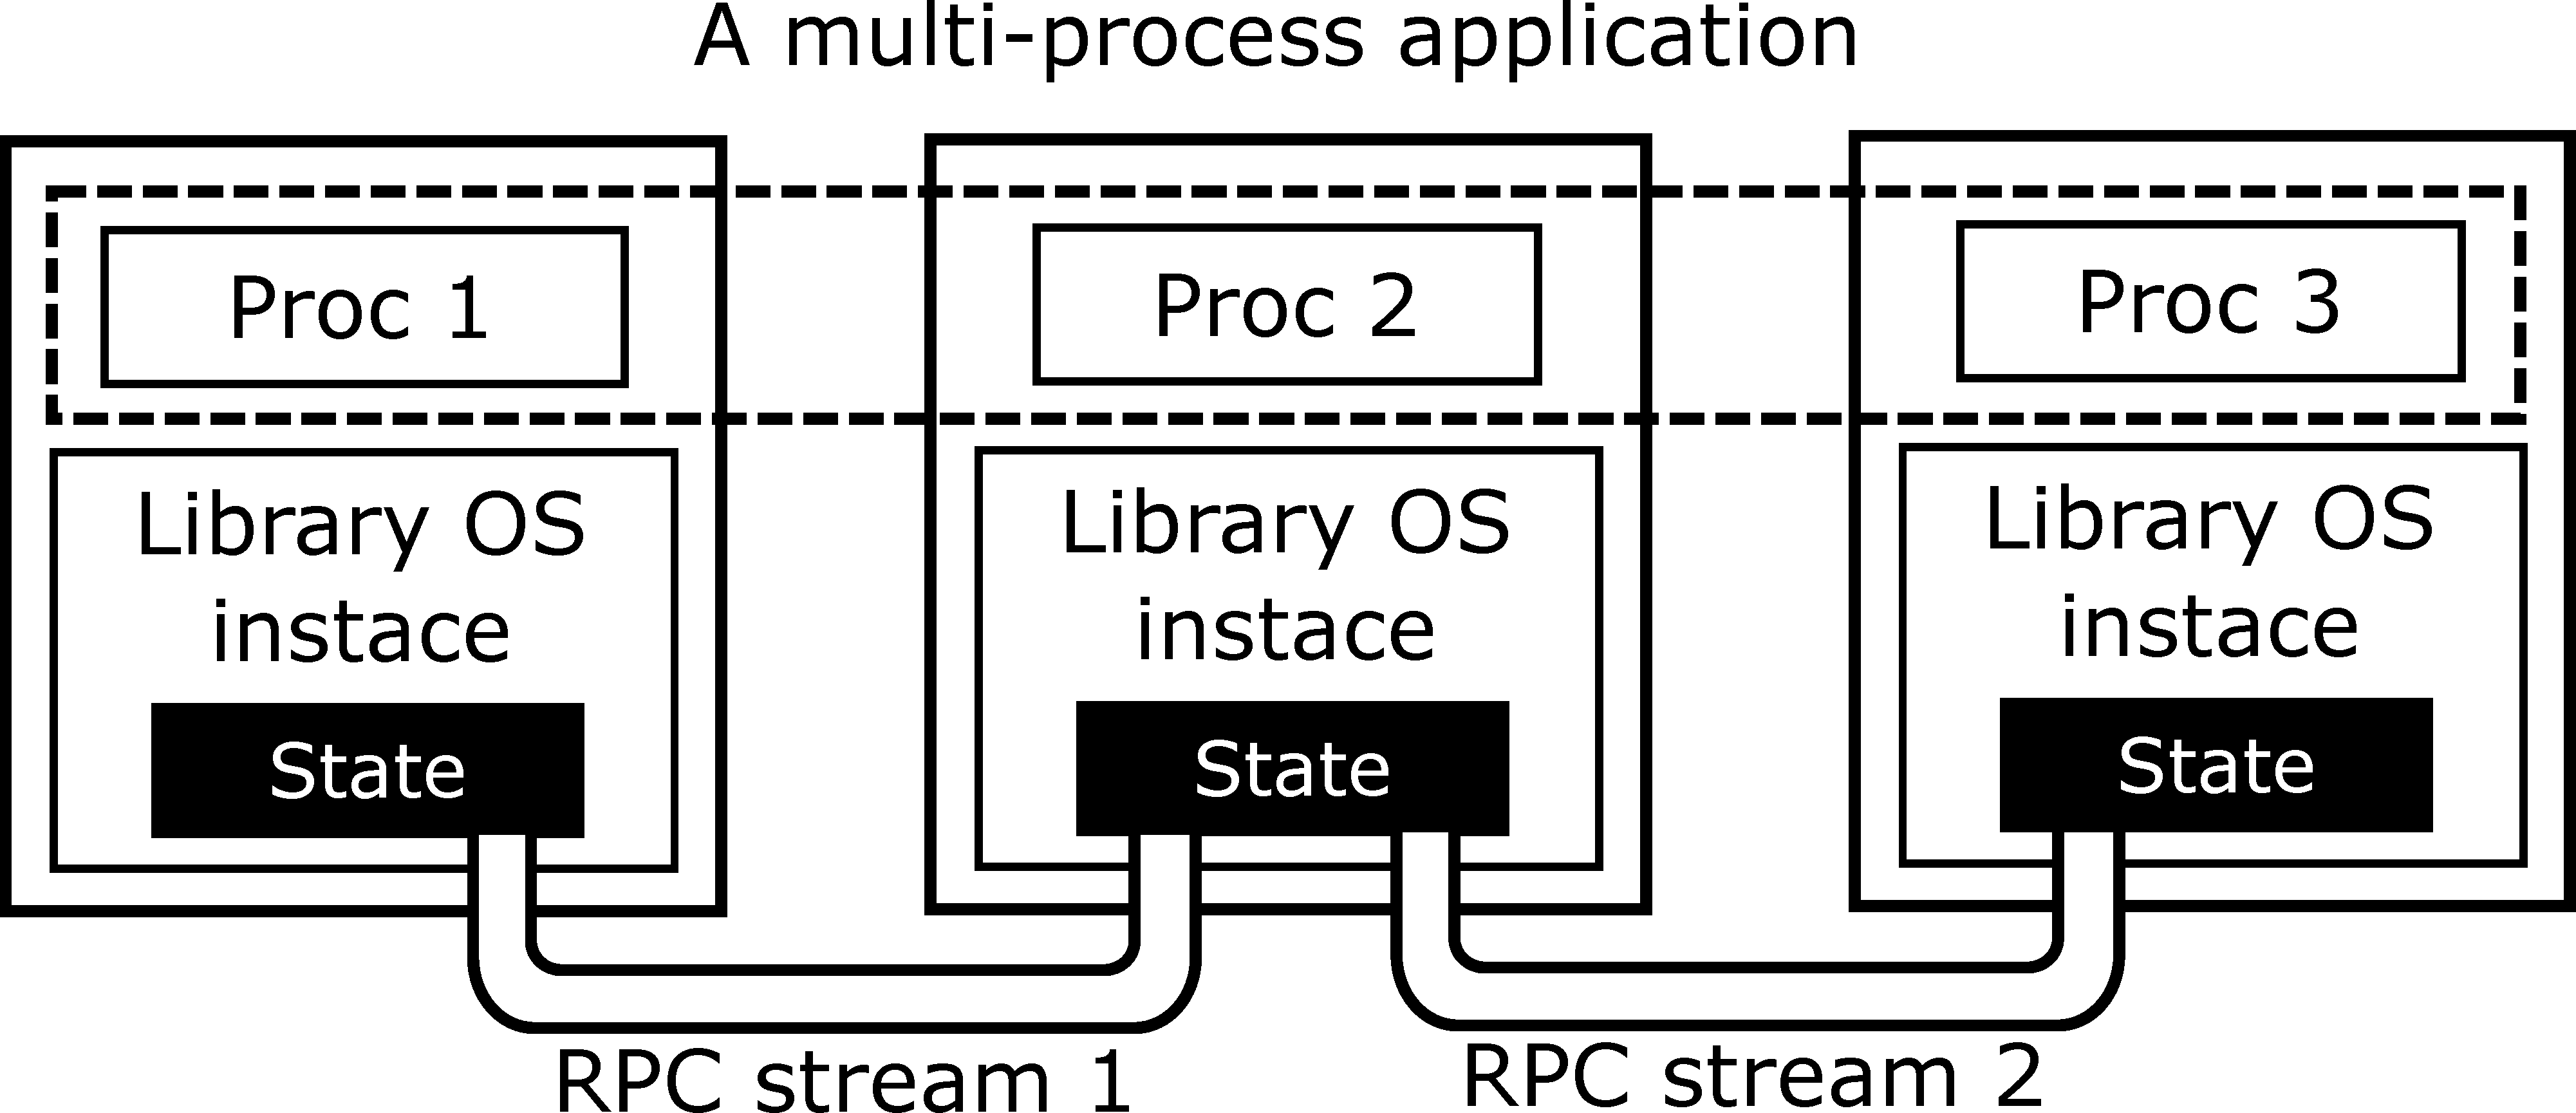
\includegraphics[width=24em]{concept.pdf}
\caption{Multi-process support model of \graphene{} \libos{}. For each process of an application, a \libos{} instance will serve system calls and keep local OS states. States of multi-process abstractions are shared by coordinating over host-provided RPC streams, creating an illusion of running in single OS for the application.}
%\vspace{-.1in}
\label{fig:graphene:concept}
\end{figure}

%{\bf \graphene{}} is a Linux-compatible library OS to run legacy, unmodified Linux applications. 
In \graphene{}, multiple library OS instances collaboratively implement
Linux abstractions, but present single, shared OS view to the application.
\graphene{} instances coordinate states
using message passing over RPC streams.
With a distributed POSIX implementation,
%placement of shared state and messaging complexity are first-order performance concerns.
%%We chose to shift implementation complexity into the library OS
%%in order to uphold simple enforcement of security isolation in the host.
%By coordinating shared states across library OS instances, 
\graphene{} can create an illusion of running in a single OS for multiple processes in an application.

%Previous library OS designs ensured security isolation of independent applications,
%comparable to a VM, by keeping a relatively narrow host ABI.
%We selected the \graphene{}
%design because it strikes a unique balance between
%and robust, flexible security enforcement.
%The \graphene{} design ensures security isolation of
%mutually distrusting, multi-process
%applications on the same host system.
%Essential to this goal is
%minimally expanding the host ABI to support multi-processing,
%as well as leveraging RPCs as a natural point to mediate inter-\picoproc{} communication.
%RPC coordination among \graphene{} instances can be dynamically disconnected, facilitating novel sandboxing
%techniques.  For instance, we develop an Apache web server extension that, upon logging in a given user,
%places the worker process's \libos{} in a sandbox with access to only that user's data.
%We expect more nuanced degrees of trust are possible in future work.

%\graphene{}'s design gives the user and system administrator a high degree of flexibility
%in isolating arbitrary groups of unmodified application processes,
%while upholding the efficiency and host compatibility benefits of recent library OSes.

%\fixmedp{After a complete draft is written, coalesce all goals and make sure they are addressed early on.  We are doing some scatter-shot motivation}


\papersubsection{\Libos{} architecture}
\label{sec:overview:libos:arch}

%Recent library OSes~\cite{porter11drawbridge,unikernels,baumann13bascule,osv}
%are designed for security and efficiency, but are limited to single-process applications.
%The security isolation of \liboses{} derives from 
%limited, explicit data sharing and 
%a narrow host interface.  
A \libos{} typically executes in either a para-virtualized VM~\cite{unikernels,osv}
% \daniela{I would have the use of a VM as a discussion topic in the end of the paper.}, 
or an OS process called a \emph{\picoproc{}}~\cite{porter11drawbridge,baumann13bascule}, with a restricted host ABI.
%The host ABI heavily restrict effects outside of the application's address space
%as a result, applications in a \picoproc{} have very little opportunity to interfere with each other,
%yielding security isolation comparable to a VM.
%The library OS deduplicates features for hardware management in both the guest and host kernels.
\graphene{} executes within a \picoproc{} (Figure~\ref{fig:overview:arch}),
which includes an unmodified application and its supporting libraries, which run alongside a library OS instance.
The \graphene{} \libos{} is implemented over \thehostabi{} designed to expose very generic abstractions that are easy to port on any host OS.
%Although the \graphene{} prototype  host kernel is Linux, 
%we adapt a host ABI from Drawbridge/Bascule,
%which has been previously implemented on \win{}, Hyper-V, and Barrelfish~\cite{porter11drawbridge,baumann13bascule,baumann09barrelfish}.
%The \graphene{} host ABI is
% summarized in Table~\ref{tab:abi} and discussed in more detail in \S\ref{sec:linux:pal}\fixmedp{if not cut...}.  
%which exposes only tens of simple host calls. \daniela{briefly define \picoproc{}: A \picoproc{} is unmodified application code running with a \libos{}.}


\begin{figure}[t]
\centering
\begin{minipage}[b]{1.25in}
\footnotesize
\raggedleft
Linux system calls \\
\graphenesyscallnum{} out of \linuxsyscallnum{}\\
\vspace{0.1in}
Host ABI \\
\palcallnum{} \hostapis{}\\
\vspace{0.2in}
\hostsyscallnum{} Linux system calls
\vspace{0.35in}
\end{minipage}
\hspace{-1.25in}
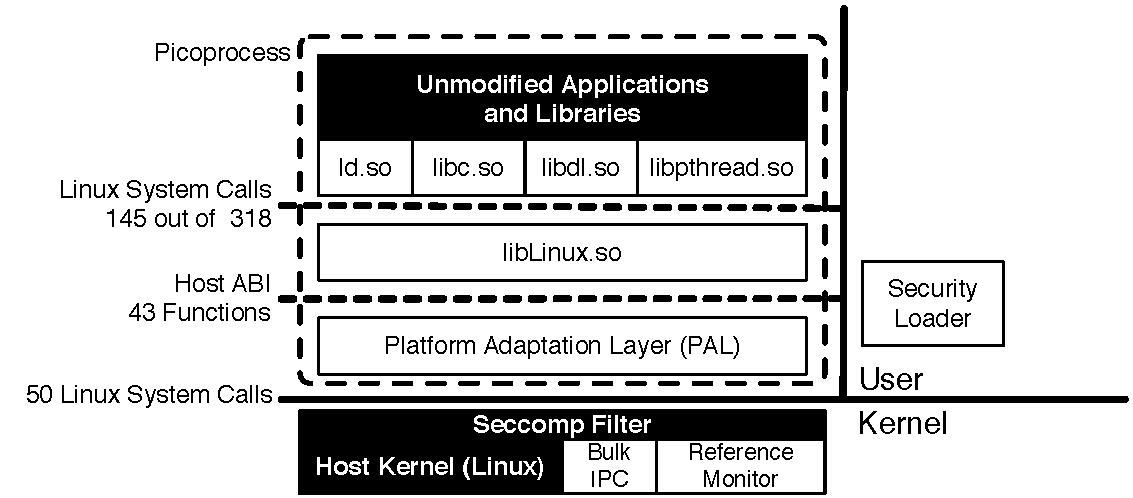
\includegraphics[width=32em]{arch.pdf}
\caption{Building blocks of \graphene{}.  Black components are unmodified.
We modify the four lowest application libraries on Linux:
{\tt ld.so} (the ELF linker and loader),
{\tt libdl.so} (the dynamic library linker),
{\tt libc.so} (standard library C),
and {\tt libpthread.so} (standard threading library), that issue Linux system calls as function calls directly to {\tt libLinux.so}.
Graphene implements the Linux system calls using a variant of the Drawbridge ABI, which is provided by the platform adaption layer (PAL).
A trusted reference monitor that ensures \libos{} isolation is implemented as a kernel module. Another small module is added for fast bulk IPC, but it is optional for hosts other than Linux.}
\label{fig:overview:arch}
\end{figure}


%\graphene{} shows the sufficiency of \thehostabi{} to support a rich Linux \libos{}.
As an example of this layering, consider the heap memory management abstraction. Linux provides applications with a data segment---a legacy abstraction dating back to original UNIX and the era of segmented memory. The primary thread's stack is at one end of the data segment, and the heap is at another.  The heap grows up (extended by \syscall{brk}) while the stack grows down until they meet in the middle.
In contrast, the host ABI provides only minimal abstractions for allocating, deallocating, and protecting regions of virtual memory.
This clean division of labor encapsulates idiosyncratic abstractions
in the library OS.


%These interfaces are host-independent \daniela{OS or kernel-independent}, as they tend to be very generic and easily
%implemented on any host OS kernel or VMM \daniela{postpone VMM for later}.

At a high level, a \libos{}
scoops the layer just below the system call table out of the OS kernel
and refactors the code as an application library.  
The driving insight is that there is a natural, functionally-narrow division point 
one layer below the system call table
in most OS kernels.
Unlike many OS interfaces, \thehostabi{} minimizes the amount of application state in the kernel, facilitating
migration. A \libos{} instance can programmatically read and modify its OS state, copy the state to another instance, and the remote instance can 
load a copy of this state into the OS---analogous to hardware registers.
A \picoproc{} may not modify another \picoprocs{}' OS states.



\papersubsection{Multi-process abstractions}
\label{sec:overview:libos:multiproc}


\issuedone{1.3.b}{An overview of multi-process support}
A key design feature of UNIX is that users compose simple utilities to create more significant applications.  Thus, it is unsurprising that many popular applications are multi-process---an essential feature missing from previous \liboses{}.
%This gap is filled by the \graphene{} \libos{}, which
%extends recent \liboses{} to support multi-process applications.
The underlying design challenge is minimally expanding a tightly-drawn isolation boundary without also exposing idiosyncratic kernel abstractions or re-duplicating mechanisms in both the host kernel and the library OS.

%requires a careful balance among the competing goals of 
%efficiency, host independence, and security isolation.
%The challenge, then, is minimal expansion of

%\vspace{5pt}
%\noindent {\bf Motivating Example.~}
For example, consider the process identifier (PID) namespace. In current, single-process library OSes, \syscall{getpid} could just return a fixed value to each application.
This single-process design is isolated, but the library OS cannot run a shell script, which requires forking and executing multiple binaries, signaling, waiting, and other PID-based abstractions.

%\paragraph{Design options.}
%Multi-process support requires extensions to the host ABI of recent, single-process library OS designs. Because multi-process abstractions, such as signals or System V IPC, tend to be idiosyncratic, an essential problem is identifying a minimal, host-independent substrate upon which  to implement OS-specific abstractions.
There are two primary design options for multi-process abstractions in \liboses{}: (1) implement processes and scheduling in 
the library OS; (2) treat each library OS instance as a process and distribute the shared POSIX implementation across a collection of library OSes.
\graphene{} follows the second option, which imposes fewer host assumptions.
%, maximize flexibility in mapping processes to physical resources, and facilitate inter-process security policy enforcement. % as enforcing security policies on related processes.

Multi-process abstractions
inside the library OS also possibly benefit from
hardware MMU virtualization, similar to
the model explored by Dune~\cite{belay12dune}.
However, this design reintroduces a duplicate scheduler and memory management.
Moreover, Intel and AMD have similar, but mutually incompatible MMU virtualization support,
which would complicate live migration across platforms.
None of these problems are insurmountable, and it would be interesting in future
work to compare both options.


In \graphene{}, multiple \liboses{} in multiple picoprocesses collaborate to implement shared abstractions. \graphene{} supports a rich of Linux multi-process abstractions including copy-on-write forking, \syscall{execve}, signals, exit notification, and System V IPC semaphores and message queues.
For instance, when process A signals process B on \graphene{}, A's library OS instance issues a query to B's instance over a pipe-like
RPC stream, and B's instance then calls the appropriate signal handler.
The host OS is unaware of the implementation
of multi-process abstractions,
as well as security isolation of the corresponding states.

%%% All collaborating \libos{} instances exchange messages as needed 
%%% to provide the application with a consistent view of 
%%% shared abstractions,
%%% such as


%\graphene{} approaches multi-processing by selectively replicating state and issuing remote procedure calls (RPCs) 
%%across multiple, collaborating
%library OS instances.
%Guests may work together to provide the unmodified multi-process application with
%coordination abstractions 

%%Shared abstractions on \graphene{}'s are implemented outside of the host, ensuring  host OS independence.
%% by implementing these
%%shared abstractions entirely
%%outside of the host kernel.
%%Shared abstractions are implemented outside of the host.
%%From the host kernel's perspective, 
%\graphene{} implements all shared abstractions by cooperatively managing the abstraction states over RPC streams.
%Single-process applications still service system calls from local state, and \graphene{}, includes optimizations to place state where it is most likely to be used, minimizing RPC overheads.
%The host reference monitor can easily isolate picoprocesses by 
%% \graphene{} design isolates \liboses{} by 
%%requiring all coordination to use 
%%explicit bytes streams \daniela{, pipe-like abstractions provided by the kernel. (suggestion: Reviewer  3)}.
%%Security isolation is enforced
%%by a kernel-level {\em reference monitor}, which can 
%%disconnect or prevent creation of a
%blocking all RPC messages, % between \liboses{} that should be isolated,
%without the need to understand the library OS details or semantics of these abstractions.
%In the PID example, only mutually-trusting picoprocesses can signal each other.
%%if the reference monitor prevents creation of RPC streams
%%across mutually untrusting \picoprocs{},
%%the \liboses{} cannot exchange signals.

%%% \graphene{} is designed to 
%%% The \graphene{} design leverages a number of optimizations to service application system calls 
%%% from local state whenever possible, and to minimize message passing overheads otherwise
%%%  (\S\ref{sec:namespaces:insights}).
%%% Our experience is that starting with a local system call design and then extending it to share state is relatively straightforward,
%%% and introduces little-to-no overhead when the request can be serviced locally.


The \graphene{} library OS is also capable of gracefully handling disconnection from other library OSes, facilitating dynamic application sandboxing.
RPC streams may disconnect at any time by either the reference monitor or at the request of a library OS.
%Message streams may be severed externally, by the reference monitor, or 
%one guest may simply disconnect from others to isolate itself.
%An application may disconnect itself from the 
%Any \graphene{} application may dynamically detach from the confederation, 
%or a host-level sandbox may dynamically separate two guests by severing their communication channels.
When a picoprocess is disconnected, the library OS will handle the subsequent
divergence, %and the library OS will will fork these abstractions
{\em transparently} to the application.
For instance, if a child process disconnect RPC streams from the parent by the reference monitor, the library OS will interpret the event as if the other process terminated, close any open pipes, and deliver exit notifications.
% \daniela{(applications run unmodified) - Reviewer 1 asked clarification on transparently}.

%% A key insight behind our design is that the common use case for these \daniela{cooperating} abstractions
%% is between a pair of processes.  Thus \graphene{} leverages a number of optimizations 
%% to reduce broadcast messages, avoid replication of needless state,
%% and service requests locally


\paragraph{Comparison with microkernels.}
The building blocks of \graphene{} are very similar to the system abstractions of a 
microkernel~\cite{liedtke95sosp,klein09sel4,elphinstone13microkernels,liedtke93sosp,chen93memory,baron1985mach-1,accetta86mach}, except a microkernel often has an even narrower, more restricted interface than the host ABI.
%such as the port and
%message abstractions of Mach~\cite{
A multi-server microkernel system, such as GNU Hurd~\cite{hurd} or Mach-US~\cite{stevenson95mach-us}, implements Unix abstractions across a set of daemons that are shared by all processes in the system. \graphene{}, on the other hand, implements system abstractions as a library in the application's address space and coordinates library state among \picoprocs{} to implement shared abstractions. \graphene{} guarantees isolation equivalent to running 
an application on a dedicated VM; it is similar to implementing the security isolation model on a multi-server microkernel by running a dedicated set of service daemons for each application.

%%% \graphene{}'s differences are motivated by two considerations: efficient support of both stand-alone, 
%%% single-process applications and multi-process applications; as well as flexible security isolation. 
%%% \graphene{} contributes techniques to seamlessly and efficiently transition 
%%% between single-process and multi-process support, as well as adapting 
%%% some known techniques to a new environment.

%The \graphene{} host ABI could be described as a hybrid microkernel, which also exposes the file system and network of the host kernel.
%Similarly, picoprocesses are assumed to be provided by a production OS, like Linux or \win{}, or by a Type 2 hypervisor.  A bare metal hypervisor could potentially export a PAL, but would require services from a trusted VM, such as Xen's dom0~\cite{barham03xen}.
%%or the \pal{} would implement more thread scheduling, networking, and file system code;
%%or the \pal{} ABI would change to push this code into the \libos{}.
%Arguably, recent library OS designs might be improved by rethinking the division of labor, but this is beyond the scope of this thesis.

%\paragraph{Alternatives.}
%Another approach to support multi-process applications in a library OS would be to use hardware MMU virtualization such as nested paging used by a system like Dune~\cite{belay12dune}
%in order to implement a second process abstraction, memory manager, and scheduler in the library OS.
%This approach threatens the efficiency benefits of deduplicating these features.
%A final option is exposing additional system interfaces, such as signals, by adding more system calls to a picoprocess. This approach undermines compatibility, as many of these coordination abstractions tend to be very OS-specific.
%%Unix signals vs.\ \win{} events, {\tt waitpid()} vs.\ blocking on a process handle, etc.
%%Although legacy OSes do enforce some access control rules on coordination abstractions,
%%kernel developers must audit and add hooks to millions of lines of code.
%%As a result,
%%users have lost confidence that a traditional OS can comprehensively enforce 
%%security isolation on these abstractions---a key motivation for using VMs
%%for security isolation.


%Systems must strike a careful balance between the competing goals of
%security isolation and multi-process coordination.
%Multi-process applications require OS-managed coordination abstractions such as signals, process exit notification, and System V IPC.
%These coordination abstractions operate within shared namespaces, such as the process ID namespace and the System V key space.
%These coordination APIs and namespaces must be consistent among coordinating processes, but can undermine security isolation among unrelated processes on the same host.
%System designs generally only meet one goal: traditional OSes have a rich but porous coordination interface, while sandboxing systems and VMs are strictly isolated.
%This thesis demonstrates that this unfortunate trade-off is not fundamental.
%coordination or isolation.  


%Traditional OS kernels typically provide  rich multi-process coordination APIs, but this richness also makes for a very porous attack surface area.  For instance, on \win{}, a program may inject libraries and create threads in another program~\cite{windows-dll-inject}; 
%similarly, unchecked file descriptor inheritance in Linux can lead to security problems~\cite{close-on-exec}.  
%Although legacy OSes do enforce some access control rules on these abstractions, kernel developers must audit and add hooks to so much code that users have lost confidence that an OS can comprehensively enforce security isolation on these abstractions.

%For achieving strong security isolation on applications, users have turned to VMs.
%For instance, if two customers host their websites in the same cloud service, the customers will insist on running their web servers in separate VMs for security.
%VMs take a heavy-handed approach to security isolation---ensuring that every application has a dedicated OS kernel in a hardware-isolated address space.
%Although virtual machines isolate applications and provide legacy OS abstractions within a VM, coordinating applications must be statically placed in the same VM,
%and cannot dynamically move to a separate VM.
%For instance, consider a web service running inside of a VM that wishes to isolate requests for different users in different VMs after authentication.  The web server administrator must statically create a VM for each user, introducing substantial
%overhead; and the developer loses convenient IPC abstractions and must rewrite large swaths of code.

\section{Summary}
\label{sec:graphene:summary}

The \graphene{} design is centered around
building a para-virtualized layer, which can reuse the OS components for reproducing Linux system interfaces.
%instead of building arbitrary compatibility layers for reproducing the system interface.
%constantly porting the significant  of the existing system interface.
%In \graphene{}, 
\graphene{} defines a host ABI, as a new boundary between the OS and user space.
The host ABI is simple enough to port (containing \palcalls{} functions),
and exports sufficient functionality for virtualizing a primary part of the system API components.
A library OS is built upon the host ABI,
and implements \graphenesyscalls{} Linux system calls to reuse unmodified Linux applications.
\graphene{} decouples the development for a compatibility layer,
from host-specific challenges to building OS features, and isolating applications from other malicious tenants.



%\sysname{} extends library OS designs 
%to include multi-process APIs required by common applications, such as a shell or 
%web server.
%\sysname{} demonstrates efficient, selective
%coordination of shared state across multiple library OS 
%instances---maintaining host independence.
%%simplifying security sandboxing of otherwise unwieldy OS features.
%Applications on \sysname{} enjoy both 
%strong security isolation with acceptable performance and low memory overheads.
%% from unrelated programs 
%%and seamless shared namespaces 
%%among a group of coordinating guests.
%%% Although this paper focuses on distributed coordination
%%% to facilitate the efficiency benefits,
%%% expect our experiences with distributed coordination 
%%% may also be particularly relevant to highly scalable OS designs, 
%%% which avoid the bottlenecks of shared OS data structures~\cite{baumann09barrelfish, song11eurosys}.
%%Graphene's overheads are acceptable and the memory 
%%footprint is substantially lower than a VM.



%% , which could benefit from the reduced memory footprint
%% in a cloud 

%% by introducing a novel design for  coordination APIs. 
%% to a new OS (Linux),
%% new classes of applications,
%% and introduces a
%% %an alternative design point for storage virtualization.
%% Our results further demonstrate the feasibility of the library OS model.
%% % generally,
%% Applications on Graphene enjoy both 
%% strong security isolation from unrelated programs 
%% and seamless shared namespaces 
%% among a group of coordinating guests.
%% Although we explore this concept in a library OS,
%% we expect the namespace coordination framework 
%% could also be adapted to limit the attack surface area between
%% processes in a traditional OS.
%% We expect these experiences with distributed coordination 
%% may also be particularly relevant to highly scalable OS designs, 
%% which avoid the bottlenecks of shared OS data structures~\cite{baumann09barrelfish}.
%and specifically of content-addressable storage as the primary virtual storage abstraction.
%%% This work opens up a number of interesting questions for future work, 
%%% including studying opportunities for low-level storage optimization within the CAS server,
%%% making CAS the root file system,
%%% eliminating storage management in the host kernel, and 
%%% investigating the impact of frequent migration among devices.

\begin{comment}
Enabling legacy applications in a restricted environment,
such as \picoprocs{} or enclaves,
requires extra effort for mitigating the limitations of platforms,
in order to support typical OS personalities.
\graphene{}, as described in this chapter, extends the existing \libos{} designs
from isolating single-process or unshared abstractions
to include multi-process APIs required by many UNIX applications,
such as servers or shell scripts.
The challenge that \graphene{} primarily overcomes
is the requirement for coordinating shared states across multiple \picoprocs{},
to provides a collaborative, unified OS view.
Essentially, \graphene{} implements all shared, multi-process abstractions
and OS states
based on coordination over host-provided, pipe-like RPC streams.
The RPC-based, distributed OS implementation enables multi-process support in \graphene{}, with minimal extension to the host interface,
and a sweet-spot for enforcing inter-application security isolation,
by simply sandboxing the RPC streams.
Such a model largely reduces the complexity of
enforcing security isolation
on idiosyncratic multi-process abstractions
and shared states.
Because the corporative nature of \picoprocs{} in \graphene{},
an application can even dynamically impose sandboxing on one of its processes,
to reflect per-process, variable security policies.
\end{comment}

\begin{comment}
In principle, we attempt to use \graphene{} to justify the platform independence
of the \libos{} design,
without sacrificing its qualitative benefits,
such as isolating mutually-untrusting applications
and a narrow attack surface to kernels.
\graphene{} implements a considerable number of common Linux system calls,
to support popular, modern applications
such as Apache web server, GNU Make, OpenJDK \java{} VM and the Python runtime.
\graphene{} translates the high-level system APIs used by applications
to a host ABI
inherited and extended from a previous Windows-compatible \libos{}~\cite{porter11drawbridge}.
In addition, we port the \pal{} (Platform Adaption Layer) of \graphene{}
to various platforms,
including FreeBSD, OSX, Windows, and even a more restricted environment, the \intel{} \sgx{} enclaves.
In particular, \graphene{} being ported to \intel{} \sgx{}
(\graphenesgx{})
can isolate applications --- either single-process or multi-process
--- on a host where neither the operating system nor the hardware (except the CPU package)
is trusted by the applications. 
Overall, \graphene{} shows that,
by simply porting the reasonably sized host ABI
to a new platform,
a whole large spectrum of legacy applications tested on the previous platforms
can be activated all together.
\end{comment}

\makeatletter
\def\input@path{{}}
\makeatother
\graphicspath{{}}
%%% dp: This title is pretty vague.  
%\section{Addressing the Combination of \java{} and \sgx{}}
\section{\java{} Support for Partitioning into \sgx{}}
\label{sec:civet:concept}

This section explains the support \sysname{} adds to \java{}
for partitioning applications into \sgx{} enclaves.
%support in addresses the challenges
%in partitioning \java{} applications on 

\subsection{Cleanly partitioning classes and objects}
\label{sec:civet:concept:partition}

%To address the partition challenge in a managed language like \java{},
%\sysname{} diminishes the need for developers
%to scrutinize the whole code base
%and identify the fine line of isolating trusted and untrusted classes. 

\sysname{} includes Shredder to automatically partition \java{} applications on \sgx{},
requiring  minimal developer effort.
Figure~\ref{fig:civet:builder} shows the workflow of a developer using the \sysname{} Shredder tool.
The developer selects the application's main class, either as a JAR or class files
and the classpath of the library.
The developer also specifies the list of
entry classes that should be in the enclave and export an interface to the code 
outside of the enclave.
%% When developers use the tool to partition their applications, they provide
%% the application package, either in JAR or classes,
%% the class paths of the depended libraries,
%% and a list of {\em entry classes} as the initial entry points of the enclave.
The Shredder then
identifies all classes that the entry classes depend upon,
until the transitive closure of these dependencies converges.
%performs {\bf dependency tracking} starting at the entry classes,
%until all the depended classes eventually converge.
%% dp: this feels out of place here; maybe put it at the beginning of the section?
%Afterward, \sysname{} packages the classes, with additional steps of augmentation, instrumentation, and signing, purpose of which is explain in \S\ref{sec:concept:loading} and \ref{sec:concept:accessing}.

\begin{figure}[t!]
\centering
\includegraphics[width=4.5in]{civet/figures/building-tool.pdf}
\caption[\sysname{}: overview of the design-time tool.]
{The \sysname{} design-time tool, for partitioning, packaging, augmentation, instrumentation, and signing.
\sysname{} partitions the \java{} application based on the entry classes
specified by the developers (classes {\tt Trusted}).
The Shredder tool recursively pulls all required supporting classes into the 
package to run in the enclave.
%from all the class paths.
%Only the minimum necessary classes are kept for the enclave,
The Shredder tool creates an enclave JAR file after augmentation,
instrumentation, and signing.}
\label{fig:civet:builder}
\end{figure}

The Shredder creates a single package with all dependencies of the
entry classes.
This is a reasonable simplification, although 
% for two reasons.  First, 
%loading all required classes from a single package is 
%is a reasonable simplification 
%that matches expected practice for enclaves.
%We note that 
it would be relatively easy in future work to add more signed JAR-style packages,
if needed.
This approach also allows us to 
reduce the attack surface and overheads by minimizing the 
enclave entry and exit points, albeit at the expense of duplicating some supporting
classes in and out of the enclave.
%\fixmedp{sounds like we don't let enclave code call out to classes? Might bear some discussion whether this is a limitation or not}

%% We argue that partition based on entry classes and
%% dependency tracking at class granularity
%% is sufficient for isolating the trusted and untrusted components.
%% There are basically two goals for our partition tool:

%% \begin{compactenum}
%% \item To create a static package of supporting classes, so \sysname{} runtime can load every required class from the package.
%% \item To avoid the isolated execution from leaving the enclave,
%% in between the entry triggered by method invocation
%% from the untrusted components,
%% and returning the control to the untrusted components.
%% \end{compactenum}


Unless the application explicitly asks the class loader to
dynamically load a class,
every piece of code needed during the execution of trusted classes
is included in the enclave image.
The image includes classes that are used in dynamic casting and parent classes 
that contain code inherited by the trusted classes.
Shredder also includes any required supporting JNI libraries in the image.
Shredder does not attempt to partition the JNI libraries to a smaller binary,
which we leave for future work.

%Because \java{} maintains type-safety in most cases \fixmedp{is it not always type safe?},
%any classes that have ever been cast to in the application can be tracked as a dependency. Methods that are inherited from the parent classes
%are also covered in dependency tracking.

%If an application will ever request for dynamic loading using class names,
%the developers must specify the classes in the partition tool.
%The case that dynamic loading is needed is most commonly seen in the crypto APIs:
%for example, to instantiate a {\tt Cipher} object,
%the applications will provide a string that describes the transformation
%of the cipher, such as {\tt AES/CBC/PKCS5PADDING}.
%Based on the string, the method {\tt Cipher.getInstance()} will load classes
%{\tt AESCipher}, {\tt PCBC}, and {\tt PKCS5Padding}.
%The rationale behind dynamic loading is that no matter
%which class name the application request for,
%the class loader will only search among the trusted classes,
%so no malicious classes will be loaded.

%% \sysname{} also includes any JNI 
%% In the case that any supporting classes require JNI,
%% \sysname{} will include the correspondent JNI libraries in the enclave image.
%% The JNI libraries are unpacked when the enclave starts,
%% and added to {\tt LD\_LIBRARY\_PATH} for the trusted \java{} VM.
%% \sysname{} currently does not partition the JNI libraries, but we see the partition of JNI as a manageable future work. 

Based on our case studies (\S\ref{sec:civet:cases}),
we observe that specifying the entry classes and identifying any dynamically loaded classes,
requires minimal developer effort.
In all of our use cases, the applications are partitioned with only one entry class, and very few dynamically loaded classes.


%\sysname{} transparently handles all the details of accessing \sgx{} hardware,
%in behave of the loaded \java{} applications (as shown in figure~\ref{fig:synthesis}).
%When \sysname{} is called to run isolated \java{} components,
%it creates two worlds of \java{} execution --- one is in the enclave and the other is outside the enclave.
%With the ability of running \java{} classes inside the enclave,
%\sysname{} can support the partitioned model with both isolated and untrusted classes implemented as \java{} classes.

%\begin{table*}[t!b!]
\centering
  \begin{tabular}{p{0.05in} >{\raggedright\arraybackslash}p{2.05in} >{\raggedright\arraybackslash}p{4.4in}}
  \toprule
  \multicolumn{2}{l}{\it Security guarantees or features} & {\it The modeling approach applied by \sysname{}} \\
  \midrule
  \midrule
  \multicolumn{3}{l}{\bf Natively provided by the \sgx{} hardware (including the SDK):} \\
  \midrule
  & Isolating security-sensitive components &
  Asking developers to identify multi-level sensitivity, by marking the {\em entry classes}. Complete separation between isolated and untrusted classes.
  \\
  \midrule
  & Secure entry / exit of enclaves &
  Exporting public methods of isolated classes. Arguments are type-checked.
  \\
  \midrule
  & Integrity of the execution environment & 
  Packaging all supporting classes into a signed JAR.
  \\
  \midrule
  & Attestation \& secure provisioning & 
  Providing class {\tt Enclave}, to create secure channels and exchange attestation.
  \\
  \midrule
  \midrule
  \multicolumn{3}{l}{\bf Improvement from combining of \java{} language and the \sgx{} hardware protection:} \\
  \midrule
  & Memory safety \& control flow integrity &
  Naturally provided by \java{} language.
  \\
  \midrule
  & Reducing the enclave TCB &
  Automated partitioning based on class dependencies.
  \\
  \midrule
  & Preventing information flow leakage &
  Tracking information flow in trusted classes, only allow releasing the information if not tainted or declassified by developers.
  \\
  \midrule
  & Code confidentiality & Dynamically loading provisioned classes.
  \\
  \end{tabular}
  
\footnotesize
\caption{
The approaches applied by \sysname{} to model the security guarantees and features of the \sgx{} hardware, and to enhance the security by combining language and hardware protections.
}
\label{tab:features}
\end{table*}


%Even though \sysname{} hides the low-level semantics of the \sgx{} hardware from the applications,
%the applications still have full access to the security guarantees ({\em what is secured?}) and features ({\em how is it secured?}) provided by the the \sgx{} hardware.
%We do so by identifying the high-level goals of these guarantees and features,
%and remodel the goals in the \java{} language.
%The underlying mechanisms of these goals is the original guarantees and features provided by the \sgx{} hardware.

%We discuss each security guarantee or features of the \sgx{} hardware,
%and how they are actually modeled in \sysname{} as follows.

%\paragraph{Isolated execution of security-sensitive components}
%The \sgx{} hardware ensures components with higher security sensitivity
%to be executed inside the enclave
%and completely isolated from the components that are less security sensitive.
%The isolated components shall not share any data with the untrusted components unless the isolated components decide
%to flow the data out of the enclave.  

%\sysname{} models this guarantee by asking the developers to make
%the classes that they believe to be security sensitive.
%Note that only the top-most classes that interact with the untrusted components have to be identified --- we can these classes as the {\em entry classes}.
%After developers identifying the multi-level security sensitive with an application, \sysname{} uses a building tool to partition the application
%based on the developers' hint.
%The partition completely separates the \java{} classes for the isolated components from the classes for the untrusted components.
%The execution of these isolated classes will be fully jailed inside the enclave, and any invocation of the methods exported by the isolated classes
%from the untrusted classes
%will be re-routed into the enclave.
%The returned values of the invoked methods will be routed back to
%the untrusted classes,
%either as proxies of the actually returned instances (if the instances are not yet safe to release from the enclave) or the actual values.



\subsection{Dynamically loading byte-code with integrity}
\label{sec:civet:concept:loading}


After the Shredder partitions the applications
and creates an enclave image as a JAR file,
developers can ship the enclave image with the rest of the application.
The application is then executed on an untrusted host with the 
%to the untrusted hosts that have the 
\sysname{} runtime framework installed.
%Then, on the untrusted hosts users will run the application,
Upon the first use, either by creating a trusted object or calling a static method of a trusted class,
%Whenever an entry class is instantiated, or one of its static method is invoked,
the \sysname{} runtime framework creates an enclave containing the trusted classes.

%\fixmedp{Trusted and isolated are used pretty interchangeably.  Pick one keyword and use it consistently, please}

Figure~\ref{fig:civet:runtime} shows the structure of the \sysname{} runtime framework(a more detailed view of Figure~\ref{fig:civet:synthesis}).
The \sysname{} runtime framework is split into the front-end (untrusted) and the back-end (trusted).
When the front-end calls into a trusted class,
it finds enclave image that contains the class,
checks if an enclave is created for the same image in the current \java{} VM,
and, if not, creates an enclave.
The trusted classes from the same image share an enclave.
%and \sysname{} does not support the scenarios that the developers want to 
%further partition the trusted classes.

\sysname{} runs a separate, lighter-weight \java{} VM in the enclave.
Running a \java{} VM in the enclave is a subtle challenge because a \java{} VM
often yields a large system API footprint, and, by default, uses a large heap. % requires access to abundant resources such as the heap.
To provide the required OS APIs inside the enclave, we use the Graphene library OS~\citep{tsai14graphene}~\footnote{Downloaded from \url{github.com/oscarlab/graphene}}.
In order to remove unneeded features and balance resource utilization with performance in current SGX enclaves, such as
a 128 MB limit on the size of the enclave page cache,
we adjust the build-time configuration of the JVM to change multithreaded garbage collector to single threaded, remove multiple JIT engines and stop non-essential threads in the JVM. 

%Moreover, a production \java{} VM like \jvm{} is implemented in
%millions of lines of code \fixme{get the actual number},
%which will cost tremendous effort to port into \sgx{} enclaves.

%To avoid the cost of porting the \java{} VM, \sysname{} uses {\em Graphene-SGX library OS}~\citep{graphene-sgx} 
%to facilitate the OS features needed by the \java{} VM.
%Therefore, we do not modify any code of \jvm{}, except tuning the compilation options to reduce its resource usage.

%\fixme{I am gonna avoid saying Graphene from now on.}
When \sysname{} creates an enclave, the \sgx{} hardware measures integrity of the initially-loaded library OS.
The library OS then loads \jvm{} and all of the supporting libraries,
such as {\tt libc},
the JLI (\java{} legacy interface) library, and the minimal \java{} classes needed to bootstrap the class loader.
Finally, \java{} VM loads the enclave image JAR file.

Graphene itself is responsible to maintain the code integrity of the JVM.
%\sysname{} depends on Graphene-SGX to maintain the code integrity.
When Graphene loads a binary or class files,
it verifies the integrity of the files by checking their measurements.
The measurements of binary or class files are also
hashed into the enclave measurement,
so no attacks can bypass the integrity check or manipulate Graphene to load  a malicious \java{} VM or bogus enclave image.

If an application requests dynamic loading by a class name,
the developers must specify the classes to the Shredder tool.
The case that dynamic loading is needed is most commonly seen in the crypto APIs:
for example, to instantiate a {\tt Cipher} object,
the applications provide a string that describes the transformation
of the cipher, such as {\tt AES/CBC/PKCS5PADDING}.
Based on the string, the method {\tt Cipher.getInstance()} loads classes
{\tt AESCipher}, {\tt PCBC}, and {\tt PKCS5Padding}.
The rationale behind this restriction on dynamic loading is that, no matter
which class name the application requests,
the class loader only searches among the trusted classes,
so no malicious classes will be loaded.
\fixmedp{Seems like you could also do a signature check at runtime, and there are other ways to relax this requirement, but whatever.}

%\paragraph{Integrity of the execution environment}
%The \sgx{} hardware must guarantee the execution of the isolated components
%is exactly the same as developed, tested and verified by the application developers.
%The \sgx{} hardware verify the cryptographic measurement of loaded binaries
%at the creation of the enclave,
%and can generate attestation that the enclave is created with such measurement.
%The purpose of the guarantee is to prevent code injection,
%unless the isolated applications are tricked into loading the code by the attackers.

%\sysname{} models this guarantee by creating a snapshot of developers'
%execution environment, including the version of \java{} VM,
%checksums of any infrastructure binaries,
%and the minimal supporting classes for the isolated component. 
%\sysname{} packs all these files into a JAR file and sign it with the developers' private key.
%When \sysname{} creates an enclave, the hardware measurement of the enclave includes only the infrastructure, as the \java{} VM and the \sysname{} back-end.
%Once the enclave is created, the \sysname{} back-end must  
%check whether the JAR file loaded has the correct signature.

\begin{figure}[t!]
\centering
\includegraphics[width=4.5in]{civet/figures/civet-structure.pdf}
\caption[\sysname{}: framework overview.]
{\sysname{} framework overview.
\sysname{} creates two worlds for an partitioned \java{} application, each with an individual JVM.
The JVM in the enclave is ported using Graphene library OS.
Untrusted classes can invoke methods of trusted classes through proxy objects,
which can transparently access the enclave interface, through serialization
and deserialization over an ring buffer accessed by both untrusted JVM and trusted JVM. }
\label{fig:civet:runtime}
\end{figure}


\subsection{Seamless access to in-enclave objects}
\label{sec:civet:concept:interface}

For programmer convenience, 
untrusted code can seamlessly call in-enclave objects in \sysname{}.
This is particularly useful when application components are closed-source.
All public methods of trusted, programmer-identified entry classes are entry points for the enclave.
The \sysname{} runtime framework is responsible for generating glue code for entering and exiting
the enclave appropriately, tracking references to objects in the enclave, 
as well as marshalling arguments and return values for in-enclave functions.

%in \sysname{},
%access to in-enclave objects seamless for the untrusted components.
%The rationale behind this design is based on two reasons.
%First, the target of method invocation in \java{} is identified dynamically
%via referencing the object.
%Second, \sysname{} intends to avoid the developers' effort for injecting explicit entry points into the untrusted components,
%especially when the imported \java{} class libraries are close-source.

%% As \sysname{} dynamically determines the enclave entry points in the untrusted components,
%% it avoids the requirement for developers
%% to define the untrusted interface of the enclave.
%% Instead of inquiring manual definition,
%% \sysname{} applies a simple principle to automatically determine the entry points:
%% All public methods of the {\em public} trusted classes can be entry points of the enclave.

In order to reference objects inside the enclave from outside the enclave,
\sysname{} framework uses a byte code generation library --- {\em CGLib}~\citep{cglib} to create untrusted proxies for the in-enclave instances.
CGLib instruments the class that is being proxied,
and redirects the control to a handler 
assigned by \sysname{} upon any method invocation on the proxy.
The proxy then triggers enclave entry to run the trusted method.



%% When untrusted code calls a public method of a trusted class,
%% \sysname{} transparently identifies 
%% determines enclave entry based on whether the objects accessed is in the enclave or part of the untrusted components.
%% As classes can be replicated inside and outside the enclave,
%% the same method of the same class must trigger different behavior according to the sensitivity of the instances.
%% If the object is instantiated in the untrusted components, the method must be run outside the enclave.
%% If the object is instantiated in the enclave, the method should be trapped,
%% and trigger enclave entry to run the method.
 
In general, supporting classes can be duplicated inside and outside of the enclave.
Calls to a supporting class, such as {\tt String}, from inside of an enclave
go to the in-enclave version, and calls from outside the enclave go to the untrusted version.

An exception is made for entry classes, which are not allowed to be replicated.
Rather, any call to an entry class function is placed inside the enclave.
Thus, constructors and static methods of entry classes also cause enclave entries.
We note that this design point was taken to minimize programmer effort in porting to SGX;
alternatively, we could allow an entry class to be replicated by requiring the programmer to 
explicitly annotate calls to object functions.

The \sysname{} design-time tool creates untrusted proxy classes for all entry classes,
in which all constructors and static methods are redirected to
the \sysname{} front-end, which then enters the enclave.
We chose this approach because CGLib disallows redirecting 
constructors and static methods, as this can introduce ambiguity in
the invocation target when all classes are in the same JVM.

%% If the method called is a constructor or static method,
%% the affected object is no longer an instance,
%% but the class itself.
%% To allow seamless invocation of the method,
%% it causes ambiguity for the affiliation of the class, if the class is replicated in both partitions.
%% Therefore, \sysname{} restricts the invocation of constructors or static methods
%% to only the entry classes,
%% and disallows replicating the entry classes
%% in the untrusted components.
%% In addition, if the constructor of an entry class is called upon the constructor of its untrusted subclass,
%% the instantiation will be rejected by \sysname{}.

%% \paragraph{Interception of in-enclave objects.}
%% To seamlessly trigger the enclave entry upon method invocation,
%% \sysname{} intercepts the instances or classes that belong to the isolated components.
%% To intercept non-static method of in-enclave instances,
%% \sysname{} uses {\em CGLib} \fixme{cite} to create proxies of the in-enclave instances.
%% CGLib instruments the class that is being proxied,
%% and redirect the control to a handler assigned by \sysname{} upon any method invocation on the proxy.
%% The handler then triggers enclave entry to run the isolated method.

%% \sysname{} uses a different mechanism of interception for constructors and static methods,
%% because CGLib disallows redirecting constructors and static method
%% due to the ambiguity of invocation targets.
%% Instead, \sysname{} uses the design-time tool to create a dummy classes for all the entry classes,
%% in which all constructors and static methods are redirected to
%% the \sysname{} front-end.
%% Because we disallow replication of entry classes
%% in the untrusted components,
%% loading the dummy classes does not affect functionalities of the application. 

\paragraph{Passing arguments into the enclave.}
When a method triggers enclave entry, the arguments of the method have to be passed into the enclave for the invocation.
\sysname{} always copy the arguments into the enclave,
by serializing the arguments into byte streams,
copying the byte streams into the enclave memory,
and then de-serializing into objects.
By coping arguments into the enclave,
\sysname{} ensures execution of trusted code does not inadvertently leave the enclave.
If the code invokes a method on one of the arguments,
the in-enclave copy of the class is used on an in-enclave instantiation of the object.
Upon de-serialization, the arguments are also automatically type-checked,
thus avoiding the risk of memory corruption.

\paragraph{Returning objects.}
Once the triggered method finishes execution in the enclave,
it may return an object or literal back to the untrusted calling function.
In general, objects are returned similarly to passing input arguments---by serializing the object to a byte stream and returning the bytes.
%Technically, returning objects is the same as passing arguments, and only take serialization and de-serialization.

In order to ensure confidentiality of sensitive data, \sysname{} takes additional care to check
whether a returned object creates an unexpected control flow.
At enclave exit, \sysname{} only allows an object to be returned if it is not tainted with any secret data,
in which case the object is serialized and passed back to the caller.
Section~\ref{sec:civet:security} details our information flow tracking mechanism.

In cases where the object is tainted and an instance of a trusted class,
\sysname{} instead creates a reference in the enclave (to prevent garbage collection of the object internally),
and returns an opaque reference type, that causes the untrusted \sysname{} runtime to create a proxy out of the enclave.
This policy applies to all constructors.
If a proxy object is garbage collected, the destructor calls into the enclave to release the reference on the 
corresponding object in the enclave.
The \sysname{} untrusted runtime is responsible for translating any proxy objects passed as arguments to the enclave into opaque pointers,
which the in-enclave runtime then translates to local object references.

In the case of a tainted literal, we encrypt the plaintext return value concatenated with a nonce, using a temporary key, and return the ciphertext.
This encrypted literal can then be passed to subsequent enclave calls, where the value is decrypted as part of deserialization.

%% However, unconditionally allowing returning objects may become a threat to the information confidentiality of the enclave,
%% because the object may contain part of the enclave secrets due to the information flow.
%% \sysname{} only allows returning objects
%% that are not tainted by the information flow from any secrets. More details about determining the taintedness of the objects are discussed in section~\ref{sec:civet:security}.

%% Based on the taintedness of the objects, \sysname{} has different policies and mechanisms of returning the objects to the caller,
%% to maintain both information confidentiality and progress of the application.
%% The policies are described as follows:

%% \begin{compactitem}
%% \item {\bf the object is not tainted}: serialize and pass the object to the caller.
%% \item {\bf the object is tainted, and is instance of an isolated class}: 
%% create a proxy and intercept future invocation.
%% The policy commonly applies to all constructors.
%% \item {\bf the object is tainted, and is a literal}:
%% automatically encrypt the literal with a default key.
%% \end{compactitem}


%\paragraph{Secure entry and exit of the enclave}
%The \sgx{} hardware ensures that the enclave only has fixed number of entry points (exactly one location where the execution starts, but multiple pre-defined locations that the execution can jump to). 
%The untrusted components must be forbidden to jump to random code in the enclave.
%Moreover, if the isolated component want to exit the enclave,
%it must explicit call the exit instruction ({\tt EEXIT}) to make sure
%the control flow won't be manipulated to leave the enclave.

%\sysname{} models this guarantees by exporting all the public methods of the isolated classes
%(including constructors, static and non-static methods) as the entry points or untrusted interfaces.
%When the untrusted component calls a constructor or static method of an isolated class,
%the execution inside the enclave is triggered,
%either to instantiate the class or perform other operations.
%If a proxy of an isolated instance is returned to the untrusted components,
%the untrusted components can keep it or pass it around.
%As soon as any untrusted components call one of the public methods on the proxy, the execution re-enter the enclave and start the isolated execution.

%Exporting public methods as the entry points or the untrusted interface
%is assumed to be reasonably secure in \sysname{}.
%First, only for the entry classes (the top-most classes of the enclave),
%the constructors or static method will be exported.
%Because developers have expressed that these classes are the ones that interact with the untrusted classes, it is safe to allow the untrusted components to calls these methods and trigger execution in the enclave.
%Second, even if the public non-static methods can be called
%upon isolated classes, the untrusted components can only call upon the proxies,
%which are essentially returned values from the previous method calls.
%Without the proxy, the untrusted components can never call the public methods
%on random instances in the enclave, if the instances are never returned to the untrusted components.


\subsection{Remote Attestation and Provisioning}
\label{sec:civet:concept:others}

\paragraph{Generating attestation reports.}
A feature of \sgx{} hardware is the ability to generate an attestation report for a remote entity,
demonstrating the integrity of the enclave code at launch time.
%The \sgx{} hardware provides the feature of generating a attestation report to prove the integrity of the isolated execution to a remote entity.
\sysname{} provides helper API for developers to access these features,
with convenience and extended trust.
For attestation, \sysname{} generates a report that contains a list of classes loaded inside the enclave, with their measurements.
The report is attached with the attestation generated and signed by \sgx{}, but processed by Graphene.
The \sgx{}-generated attestation contains both
the enclave measurement (proving integrity of Graphene) and
the measurement verified by Graphene (proving integrity of other binaries and files).


%% \fixmedp{Huh?  Really?}
%% The attestation report contains the enclave measurement
%% and is signed using a key derived
%% from the measurements of both sides of attesters,
%% so the remote entity can verify it by retrieving the same key
%% (both attesters must be running in \sgx{} enclaves).

Note that \sysname{} also includes
the dynamic loading state in the attestation report.
%A stronger guarantee provided by \sysname{} than \sgx{}
%is to present the dynamic loading state in the attestation report.
The attestation generated by \sgx{} only contains
the initial state of the enclave, and does not record changes within the executable code
after the enclave starts. 
In both cases, the remote entity is trusting the initially loaded binary
to not dynamically load code that could compromise the enclave;
however, \sysname{} can offer a more precise accounting of the state of the enclave 
at the time a report is generated.

\fixmedp{For future work, would be cool to have some non-editable record of what is added to the enclave, so a corrupted enclave cannot hide the equivalent of a rootkit}

%% As a result, the entity that
%% verifies the attestation report has to blindly trust the initial code
%% in the enclave does not dynamically load any vulnerable code.  
%% The attestation report generated by \sysname{}
%% reflects the latest state of class loading,
%% allowing the trusted entity to audit the execution of enclaves.

% providing a class called {\tt Enclave}, with the APIs that service attestation and provisioning requests.
%The {\tt Enclave} APIs are wrapper to the low-level semantics required by the \sgx{} hardware,such as exchanging the attestations with remote hosts and verifying them, or 
%securing the channels after attesting the other side of communication.
%Because the works are completely hidden beneath the APIs,
%the developers are spared from all the cryptographic details during the process of attestation and provisioning.

\paragraph{Secure provisioning.}
\sysname{} provides an API that transparently validates a connection to a remote host to load
sensitive classes or secret data.
%to be used for secure provisioning.
To use this API, both sides of the connection
must be running in enclaves created by \sysname{}.
The API performs key exchange algorithm (e.g., Diffie-Hellman) on the connection,
secure the connection with encryption,
and authenticate the connection by exchanging the attestation reports.
\sysname{} provides convenient helper functions for developers to create a trusted path
for provisioning sensitive data to a remote enclave.
%Developers can use this API to design any provisioning scheme, without implementing the details of building the trusted path.


\section{Hardening \sgx{} at Enclave Boundary using Information Flow Control in \java{} }
\label{sec:civet:security}

\sysname{} % models the high-level security guarantees and features
%of the \sgx{} hardware in the \java{} language,
allows \java{} developers to directly utilize the security features of \sgx{}, such as isolation from an untrusted hypervisor, % execution, code integrity, etc,
in combination with language-level features that make the code in the enclave more robust.
% safety and advanced protections in \java{}.
%By bridging the gap between language and hardware protections,
%\sysname{} creates opportunities to combine \sgx{} hardware protections
%and security benefits given by \java{} as a managed language.
%In this section, we discussed the opportunities we explore to harden \sgx{} protection with the usage of \java{} language.

%\fixmedp{Honestly, a lot of this is getting pretty repetitive.  I would probably hoist the argument for Java into the motivational text and not bother repeating it here.}

%\subsection{Benefits from the usage of \java{} Language}

%We note that \java{} has several features that can reduce or eliminate
%common vulnerabilities.
%Memory corruption bugs are constant threats to applications
%implemented in C or C++ languages,
%but \java{} applications naturally defend against these vulnerabilities.
%\java{} is immune from memory corruption bugs, such as heap and buffer overflows.
%Several security enhancements come naturally with running \java{} classes
%in the enclave. \java{} applications are known to be immune to memory corruption bugs such as buffer or heap overflow.
%Type casting in \java{} is checked against the type of the target object.
%applications, \java{} perform strict type-checking on the objects to be casted.
%Type-checking prevents corruption of object either in the isolated components,
%or when receiving arguments from the untrusted interfaces.
%Similarly, 
%Similar as the memory corruption bugs,
%Because \java{} is memory safe, it is immune to known control flow attacks, such as return-oriented programming,
%where control flow is manipulated by unsafe writes to return pointers on the stack or function pointers in objects.
%applications implemented in C or C++ languages inevitably face the risk of ROP (return-oriented programming) attacks,
%where attackers can manipulate the control flow by corrupting the applications' stacks or heaps.
%Since \java{} classes can defend against memory corruption,
%attacks cannot manipulate the control flow by overriding the return pointers or function pointers.

%We do assume that the JVM and JNI code are free from memory corruption and control flow attacks.
%Proving a JVM implementation correct is beyond the scope, although similar 
%efforts have been made previously to prove a language runtime correct~\citep{yang10safe}.
%In the case of JNI, we would discourage developers from using JNI code in enclaves if at all possible.

%% Note that although memory corruption bugs and control flows attacks are forbidden in \java{} classes,
%% these vulnerabilities can still exist in the \java{} VM and JNI.
%% In \sysname{} we assume \java{} VM and JNI must be fully trusted,
%% and we leave it as a future work to secure these components.

%% dp: Meh.  prolix
%% For isolated components in the enclaves, memory corruption bugs and control flow attacks are just as dangerous as for other applications.
%% Because the isolated components are fully trusted by the CPU,
%% they can access any memory that are set to proper permissions, including the memory outside the enclaves.
%% Even if a vulnerable component is exploited to copy all the enclave secret out of the enclaves, no hardware solution can effectively stop the exploitation.
%% Even though isolated components cannot directly jump out of the enclave,
%% control flow attack can still manipulate the components to jump to certain locations internally and perform malicious operations. 
%% Therefore, preventing memory corruption bugs and control flow attacks
%% can be a strong reason for application developers
%% to choose \java{} language instead of C/C++ to implement the isolated components.

%\fixmedp{This whole subsection is already covered above.  Commenting}
\begin{comment}
\subsection{Reducing the enclave TCB}

%A \java{} applications often yield a huge TCB, including the \java{} VM,
%JNI and supporting classes that come in bulk.
%For example, a \java{} applications executed by \jvm{}
%will load the \java{} VM binaries up to 40MB \fixme{find out actual numbers}. The classes in the standard \java{} VM libraries such as {\tt rt.jar} includes more than 18,000 classes, and the size of the package is more than 30MB.
%On the other hand, the actual classes needed by an application from {\tt rt.jar}
%can be as less as 1,000 classes.
%Majority of the classes provided from {\tt rt.jar},
%--- even though they may never be loaded into the enclave ---
%still remains in the TCB.

Having unnecessary binaries and classes in the TCB of the enclave
can aggravate the risk of being attacks.
First of all, the huge amount of code loaded into the enclave
increase the opportunity of having gadgets that can be exploited in ROP attacks,  
which can still happen in the \java{} VM or JNI.
Even though most of the \java{} classes have static footprint of their supporting classes,
many of them still dynamically load classes, such as directly calling the class loader, or specifying providers to the \java{} cryptography framework.
Having huge TCB as \java{} classes in the enclave still intensify
the risk of attacks, even though \java{} classes are immune to control flow attacks. 

\sysname{} largely reduce the supporting classes that can be loaded into the enclave,
by partitioning out the necessary classes from all the libraries in the developers' class paths, into the enclave image.
When the enclave is created, the \java{} VM will not load any existing libraries such as {\tt rt.jar} from the host system,
but instead only search classes in the signed enclave image.
Minimizing the supporting classes that can be loaded into the enclave
guarantees that all the classes that are included in the TCB
are actually required by the isolated components,
and come from a trusted source such as the developers' execution environment. 

Note that we do not partition the JNI within the \java{} VM binaries.
We assume partitioning out the JNI functions that are required by the isolated classes
is fully feasible with some manageable efforts.
Moreover, the \java{} classes can be potentially partitioned at a smaller granularity than the whole classes, such as the methods and fields, which can even further reduce the TCB.
We leave these potential improvements as future works. 
\end{comment}

%\subsection{Information Flow Control at Enclave Boundary}
%Problem of not just leaking secrets but also tainted info
As an example of higher-level, language-based analysis, we implemented information flow tracking
in \sysname{}.
A common usage of enclaves is to protect sensitive data, such as an encryption key;
thus, a common concern is that this sensitive data not be inadvertently returned because of an error or exploit within the enclave code.
In general, we chose a design point that minimizes programmer effort; to adopt information flow tracking, we
do require the programmer to specify secret data classes and declassify objects to be released as is from the enclave.

\begin{figure}[t!]
\centering
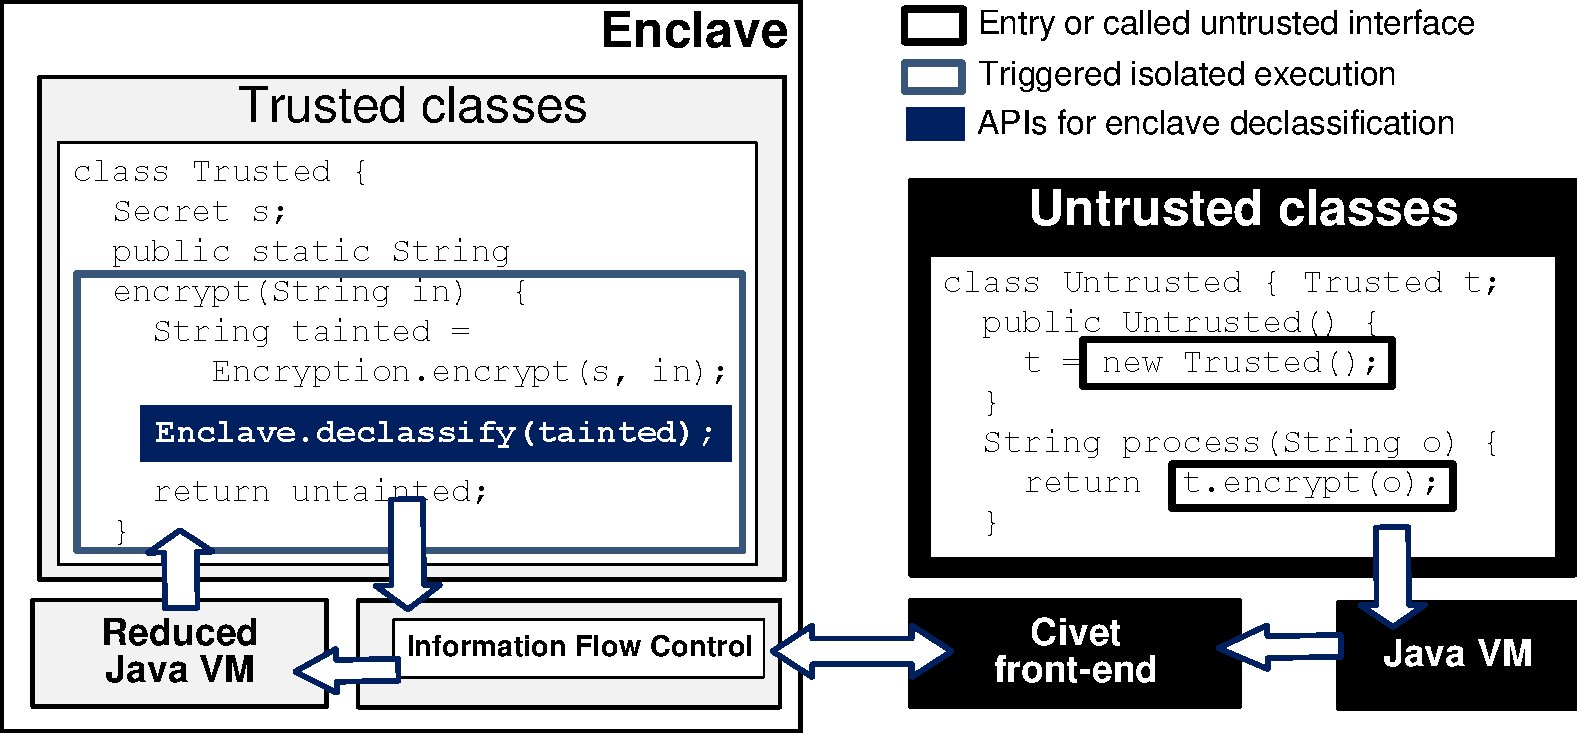
\includegraphics[width=3.2in]{civet/figures/declassify.pdf}
\footnotesize
\caption[\sysname{}: declassifier APIs.]
{How \sysname{} provides declassifier APIs to declassify sensitive data.
When the untrusted class ({\tt Untrusted}) from Figure ~\ref{fig:civet:synthesis} now calls the {\tt encrypt} method of a trusted class ({\tt Trusted}),
\sysname{} automatically calls the {\tt encrypt} method inside enclave, and pass the {\tt String} parameter.
Before returning the result, the trusted class has to use the {\tt declassify} to remove the taint of {\tt tainted} variable that is tainted by the {\tt encrypt} method of class {\tt Encryptor} because of the tainted secret variable {\tt s}.
}
\label{fig:civet:declassify}
\end{figure}

%Because the code running in enclave has access to complete address space, including the trusted as well as untrusted memory regions, it is easy for the trusted code to inadvertently undermine \sgx{} protection by writing secret information in the untrusted region. Further, leaking any information derived from or related to the secret may be used by the untrusted code to guess the value of secret information. For example, even in the presence of memory protection, sandboxing and virtualization, it is possible to recover the secret key used by crypto algorithms~\citep{kocher1996timing,osvik2006cache,weiss2012cache, zhang2012cross}. So, to ascertain the secrecy of the sensitive data, no information derived from the secret should exit enclave in plaintext.

%We use JAVA tool phosphor source and sink to taint provisioned data and control leakage
%\sysname{} leverages extensive research on information flow tracking and control in \java{} to harden the \sgx{} security. 

In the enclave, we implement source-to-sink taint tracking, using the open-source Phosphor library~\citep{phosphor}.
%\fixmedp{check this}
The programmer manually selects the classes containing secret data that take secret input from a remotely-provisioned source.
This taint is propagated to any new variables that result from explicit or implicit flows from a secret object.
The only way to remove taint from an object is to pass the object through a \sysname{} declassifier API,
which returns an untainted copy of the object.

%\fixmedp{Would be nice to have a simple example class with a label and declassifier in a figure, if space and time allow}

\sysname{} enforces the policy that only untained data may be returned from an enclave.
If tainted data is being returned, the system transparently encrypts the data and removes its taint before letting the data leave the enclave.
In the cases where a developer wants to return references to sensitive data, \sysname{} instead returns an opaque reference or, in the case of a literal, encrypts the return value.

%mFor tainted data, the developer may opt to either throw a runtime error, or, by default, to return an encrypted object instead.
%The en

% to taint the secret data when provisioned and propagate the taint to any new data generated as an explicit or implicit result of the secret data. We specify the enclave exit points as targets and enforce the policy that any tainted data must pass through a declassifier, that encrypts the data before egress. We only consider the provisioned data as security sensitive, as the enclave image is only integrity protected.

%Declassifier API: correct usage and scenarios
The \sysname{} {\tt Enclave} class provides a {\tt declassify(Object o)} API that creates an untainted
copy of the object.  In practice, we expect this function to be used in conjunction with tests
on the returned data, or cryptographic functions to protect the data in transit across an untrusted channel.

Continuing our example from Figure~\ref{fig:civet:synthesis}, in Figure~\ref{fig:civet:declassify}, if the {\tt Untrusted} class wants to call the {\tt encrypt} method on the trusted object {\tt t}, \sysname{} front-end transparently passes the argument string {\tt o} to the enclave, and the corresponding {\tt encrypt} method is called in the enclave. The secret {\tt s} is tainted because it was provisioned from remote trusted server as shown in Figure ~\ref{fig:civet:synthesis}. As a result, the call to method {\tt encrypt} of class {\tt Encryptor} taints the encrypted output string {\tt tainted}. If the developer had returned this {\tt tainted} variable, the \sysname{} information flow tracking would re-encrypt the ciphertext, and thus make the return value useless for the {\tt Untrusted} class. However, as the developer wants to return the ciphertext as is, she can declassify the {\tt tainted} string by passing it through the declassifier API to get an untainted version of the same object. Such untainted objects can be released from the enclave without further encryption.

%to let the application developer explicitly indicate that the argument object does not contain any secret information, and is safe to leave the enclave as is. For instance, if the enclave code encrypts a blob of data using the tainted secret provisioned key, the information flow will taint the encrypted data. However, because the encrypted data is safe to exit enclave if a perfectly secure encryption algorithm is used, the developer can explicitly mark the encrypted data as declassified. We note that the developers need to be extra careful while declassifying objects to inadvertently leaking secret information.

%Dealing with confidential code
In order to protect the confidentiality of sensitive code,
\sysname{} also allows classes themselves to be tainted.
\sysname{} enforces a policy that any data returned from sensitive code is tainted, and the developer needs to explicitly declassify tainted output data to mitigate
concerns around reverse-engineering the code based on brute-force probing of its outputs.
Of course, the binary code itself is also not allowed to be copied out of the enclave.

% expose it to the untrusted world.
%The {\em code confidentiality} property of \sysname{} loads and executes encrypted classes from remote hosts to protect secret algorithm. We consider this provisioned code as equally security sensitive as provisioned data. ~

%\begin{table*}[t!b!]
\centering
  \begin{tabular}{p{0.05in} >{\raggedright\arraybackslash}p{2.05in} >{\raggedright\arraybackslash}p{4.4in}}
  \toprule
  \multicolumn{2}{l}{\it Security guarantees or features} & {\it The modeling approach applied by \sysname{}} \\
  \midrule
  \midrule
  \multicolumn{3}{l}{\bf Natively provided by the \sgx{} hardware (including the SDK):} \\
  \midrule
  & Isolating security-sensitive components &
  Asking developers to identify multi-level sensitivity, by marking the {\em entry classes}. Complete separation between isolated and untrusted classes.
  \\
  \midrule
  & Secure entry / exit of enclaves &
  Exporting public methods of isolated classes. Arguments are type-checked.
  \\
  \midrule
  & Integrity of the execution environment & 
  Packaging all supporting classes into a signed JAR.
  \\
  \midrule
  & Attestation \& secure provisioning & 
  Providing class {\tt Enclave}, to create secure channels and exchange attestation.
  \\
  \midrule
  \midrule
  \multicolumn{3}{l}{\bf Improvement from combining of \java{} language and the \sgx{} hardware protection:} \\
  \midrule
  & Memory safety \& control flow integrity &
  Naturally provided by \java{} language.
  \\
  \midrule
  & Reducing the enclave TCB &
  Automated partitioning based on class dependencies.
  \\
  \midrule
  & Preventing information flow leakage &
  Tracking information flow in trusted classes, only allow releasing the information if not tainted or declassified by developers.
  \\
  \midrule
  & Code confidentiality & Dynamically loading provisioned classes.
  \\
  \end{tabular}
  
\footnotesize
\caption{
The approaches applied by \sysname{} to model the security guarantees and features of the \sgx{} hardware, and to enhance the security by combining language and hardware protections.
}
\label{tab:features}
\end{table*}


%% dp: This title is pretty vague.  
%\section{Addressing the Combination of \java{} and \sgx{}}
\section{\java{} Support for Partitioning into \sgx{}}
\label{sec:concept}

%\fixmets{1.5 page}

This section explains the support \sysname{} adds to \java{}
for partitioning applications into \sgx{} enclaves.
%support in addresses the challenges
%in partitioning \java{} applications on 

\subsection{Cleanly partitioning classes and objects}
\label{sec:concept:partition}

%To address the partition challenge in a managed language like \java{},
%\sysname{} diminishes the need for developers
%to scrutinize the whole code base
%and identify the fine line of isolating trusted and untrusted classes. 

\sysname{} includes Shredder to 
 partition \java{} code for \sgx{},
reducing developer effort.
Figure~\ref{fig:builder} shows the workflow of a developer using the \sysname{} Shredder tool.
The developer selects the application's main class, either as a JAR or class files
and the classpath of the library.
The developer also specifies the list of
entry classes that should be in the enclave and exports an interface to the code 
outside of the enclave.
%% When developers use the tool to partition their applications, they provide
%% the application package, either in JAR or classes,
%% the class paths of the depended libraries,
%% and a list of {\em entry classes} as the initial entry points of the enclave.
The Shredder then
identifies all classes that the entry classes depend upon,
until the transitive closure of these dependencies converges.
%performs {\bf dependency tracking} starting at the entry classes,
%until all the depended classes eventually converge.
%% dp: this feels out of place here; maybe put it at the beginning of the section?
%Afterward, \sysname{} packages the classes, with additional steps of augmentation, instrumentation, and signing, purpose of which is explain in \S\ref{sec:concept:loading} and \ref{sec:concept:accessing}.

\begin{figure}[t!]
\centering
\includegraphics[width=1.0\linewidth]{building-tool.pdf}
\caption{\sysname{} \staticphase{} tool, for partitioning, packaging, augmentation, instrumentation, and signing.
\sysname{} partitions the \java{} application based on the entry classes
specified by the developers (classes {\tt Trusted}).
The Shredder tool recursively pulls all required supporting classes into the 
package to run in the enclave.
%from all the class paths.
%Only the minimum necessary classes are kept for the enclave,
The Shredder tool creates an enclave JAR file after augmentation,
instrumentation, and signing.}
\label{fig:builder}
\end{figure}

The Shredder creates a single package with all dependencies of the
entry classes.
This is a reasonable simplification, although 
% for two reasons.  First, 
%loading all required classes from a single package is 
%is a reasonable simplification 
%that matches expected practice for enclaves.
%We note that 
it would be relatively easy in future work to add multiple, signed JAR-style packages,
if needed.
This approach also allows us to 
reduce the attack surface and overheads by minimizing the 
enclave entry and exit points, albeit at the expense of duplicating some supporting
classes in and out of the enclave.
%\fixmedp{sounds like we don't let enclave code call out to classes? Might bear some discussion whether this is a limitation or not}

%% We argue that partition based on entry classes and
%% dependency tracking at class granularity
%% is sufficient for isolating the trusted and untrusted components.
%% There are basically two goals for our partition tool:

%% \begin{compactenum}
%% \item To create a static package of supporting classes, so the \sysname{} \dynamicphase{} framework can load every required class from the package.
%% \item To avoid the isolated execution from leaving the enclave,
%% in between the entry triggered by method invocation
%% from the untrusted components,
%% and returning the control to the untrusted components.
%% \end{compactenum}


Unless the application explicitly asks the class loader to
dynamically load a class,
every piece of code needed during the execution of trusted classes
is included in the enclave image.
The image includes classes that are used in dynamic casting and parent classes 
that contain code inherited by the trusted classes.
Shredder also includes any required supporting JNI libraries in the image.
Shredder does not attempt to partition the JNI libraries to a smaller binary,
which we leave for future work.

%Because \java{} maintains type-safety in most cases \fixmedp{is it not always type safe?},
%any classes that have ever been cast to in the application can be tracked as a dependency. Methods that are inherited from the parent classes
%are also covered in dependency tracking.

%If an application will ever request for dynamic loading using class names,
%the developers must specify the classes in the partition tool.
%The case that dynamic loading is needed is most commonly seen in the crypto APIs:
%for example, to instantiate a {\tt Cipher} object,
%the applications will provide a string that describes the transformation
%of the cipher, such as {\tt AES/CBC/PKCS5PADDING}.
%Based on the string, the method {\tt Cipher.getInstance()} will load classes
%{\tt AESCipher}, {\tt PCBC}, and {\tt PKCS5Padding}.
%The rationale behind dynamic loading is that no matter
%which class name the application request for,
%the class loader will only search among the trusted classes,
%so no malicious classes will be loaded.

%% \sysname{} also includes any JNI 
%% In the case that any supporting classes require JNI,
%% \sysname{} will include the correspondent JNI libraries in the enclave image.
%% The JNI libraries are unpacked when the enclave starts,
%% and added to {\tt LD\_LIBRARY\_PATH} for the trusted \jvm{}.
%% \sysname{} currently does not partition the JNI libraries, but we see the partition of JNI as a manageable future work. 

Based on our case studies (\S\ref{sec:case-study}),
we observe that specifying the entry classes and identifying any dynamically loaded classes,
is relatively simple.  %requires low developer effort.
In all of our use cases, the applications are partitioned with only one entry class, and very few dynamically loaded classes.


%\sysname{} transparently handles all the details of accessing \sgx{} hardware,
%in behave of the loaded \java{} applications (as shown in figure~\ref{fig:synthesis}).
%When \sysname{} is called to run isolated \java{} components,
%it creates two worlds of \java{} execution --- one is in the enclave and the other is outside the enclave.
%With the ability of running \java{} classes inside the enclave,
%\sysname{} can support the partitioned model with both isolated and untrusted classes implemented as \java{} classes.

%\begin{table*}[t!b!]
\centering
  \begin{tabular}{p{0.05in} >{\raggedright\arraybackslash}p{2.05in} >{\raggedright\arraybackslash}p{4.4in}}
  \toprule
  \multicolumn{2}{l}{\it Security guarantees or features} & {\it The modeling approach applied by \sysname{}} \\
  \midrule
  \midrule
  \multicolumn{3}{l}{\bf Natively provided by the \sgx{} hardware (including the SDK):} \\
  \midrule
  & Isolating security-sensitive components &
  Asking developers to identify multi-level sensitivity, by marking the {\em entry classes}. Complete separation between isolated and untrusted classes.
  \\
  \midrule
  & Secure entry / exit of enclaves &
  Exporting public methods of isolated classes. Arguments are type-checked.
  \\
  \midrule
  & Integrity of the execution environment & 
  Packaging all supporting classes into a signed JAR.
  \\
  \midrule
  & Attestation \& secure provisioning & 
  Providing class {\tt Enclave}, to create secure channels and exchange attestation.
  \\
  \midrule
  \midrule
  \multicolumn{3}{l}{\bf Improvement from combining of \java{} language and the \sgx{} hardware protection:} \\
  \midrule
  & Memory safety \& control flow integrity &
  Naturally provided by \java{} language.
  \\
  \midrule
  & Reducing the enclave TCB &
  Automated partitioning based on class dependencies.
  \\
  \midrule
  & Preventing information flow leakage &
  Tracking information flow in trusted classes, only allow releasing the information if not tainted or declassified by developers.
  \\
  \midrule
  & Code confidentiality & Dynamically loading provisioned classes.
  \\
  \end{tabular}
  
\footnotesize
\caption{
The approaches applied by \sysname{} to model the security guarantees and features of the \sgx{} hardware, and to enhance the security by combining language and hardware protections.
}
\label{tab:features}
\end{table*}


%Even though \sysname{} hides the low-level semantics of the \sgx{} hardware from the applications,
%the applications still have full access to the security guarantees ({\em what is secured?}) and features ({\em how is it secured?}) provided by the the \sgx{} hardware.
%We do so by identifying the high-level goals of these guarantees and features,
%and remodel the goals in the \java{} language.
%The underlying mechanisms of these goals is the original guarantees and features provided by the \sgx{} hardware.

%We discuss each security guarantee or features of the \sgx{} hardware,
%and how they are actually modeled in \sysname{} as follows.

%\paragraph{Isolated execution of security-sensitive components}
%The \sgx{} hardware ensures components with higher security sensitivity
%to be executed inside the enclave
%and completely isolated from the components that are less security sensitive.
%The isolated components shall not share any data with the untrusted components unless the isolated components decide
%to flow the data out of the enclave.  

%\sysname{} models this guarantee by asking the developers to make
%the classes that they believe to be security sensitive.
%Note that only the top-most classes that interact with the untrusted components have to be identified --- we can these classes as the {\em entry classes}.
%After developers identifying the multi-level security sensitive with an application, \sysname{} uses a building tool to partition the application
%based on the developers' hint.
%The partition completely separates the \java{} classes for the isolated components from the classes for the untrusted components.
%The execution of these isolated classes will be fully jailed inside the enclave, and any invocation of the methods exported by the isolated classes
%from the untrusted classes
%will be re-routed into the enclave.
%The returned values of the invoked methods will be routed back to
%the untrusted classes,
%either as proxies of the actually returned instances (if the instances are not yet safe to release from the enclave) or the actual values.



\subsection{Dynamically loading byte-code with integrity}
\label{sec:concept:loading}

A key motivation for dynamic loading is the ability to load encrypted
classes from a remote, trusted host. 
For instance, one may want to load proprietary code into an enclave
that must first be decrypted and then validated, in order to 
protect an implementation of a trade secret.

Shredder creates a partition image as a JAR file, which
developers can ship with the rest of the application.
The application is then executed on an untrusted host with the 
%to the untrusted hosts that have the 
\sysname{} \dynamicphase{} framework installed.
%Then, on the untrusted hosts users will run the application,
Upon the first use, either by creating a trusted object or calling a static method of a trusted class,
%Whenever an entry class is instantiated, or one of its static method is invoked,
the \sysname{} \dynamicphase{} framework creates an enclave containing the trusted classes.

%\fixmedp{Trusted and isolated are used pretty interchangeably.  Pick one keyword and use it consistently, please}

Figure~\ref{fig:runtime} shows the structure of the \sysname{} \dynamicphase{} framework (a more detailed view of Figure~\ref{fig:synthesis}).
The \sysname{} runtime framework is split into the front-end (untrusted) and the back-end (trusted).
When the front-end calls into a trusted class,
it finds enclave image that contains the class,
checks if an enclave is created for the same image in the current \jvm{},
and, if not, creates an enclave.
The trusted classes from the same image share an enclave.
%and \sysname{} does not support the scenarios that the developers want to 
%further partition the trusted classes.

\sysname{} runs a separate, lighter-weight \jvm{} in the enclave.
Running a \jvm{} in the enclave is a subtle challenge because a \jvm{}
often yields a large system API footprint, and, by default, uses a large heap. % requires access to abundant resources such as the heap.
To provide the required OS APIs inside the enclave, we use the \graphene{} \libos{}~\cite{tsai14graphene}~\footnote{Downloaded from \url{github.com/oscarlab/graphene}}.
In order to remove unneeded features and balance resource utilization with performance in current \sgx{} enclaves, such as
a 128 MB limit on the size of the enclave page cache,
we adjust the build-time configuration of the \jvm{} to change multi-threaded garbage collector to single threaded, remove multiple JIT engines and stop non-essential threads in the \jvm{}. 
\fixmedp{say how, more specifically (in English.  You don't need to list specific options, but give us a bit more here}

%Moreover, a production \jvm{} like \jvmname{} is implemented in
%millions of lines of code \fixmets{get the actual number},
%which will cost tremendous effort to port into \sgx{} enclaves.

%To avoid the cost of porting the \jvm{}, \sysname{} uses {\em \sgx{}-\sgx{} \sgx{}}~\cite{graphene-sgx} 
%to facilitate the OS features needed by the \jvm{}.
%Therefore, we do not modify any code of \jvmname{}, except tuning the compilation options to reduce its resource usage.

%\fixmets{I am gonna avoid saying \sgx{} from now on.}
When \sysname{} creates an enclave, the \sgx{} hardware measures integrity of the initially-loaded \libos{}.
The \libos{} then loads \jvmname{} and all of the supporting libraries,
such as {\tt libc},
the JLI (\java{} legacy interface) library, and the minimal \java{} classes needed to bootstrap the class loader.
Finally, \jvm{} loads the enclave image JAR file.

The \graphene{} \libos{} maintains the code integrity of the \jvm{}.
When \graphene{} loads a binary or class files,
it verifies the integrity of the files by checking their measurements.
The measurements of binary or class files are also
hashed into the enclave measurement,
so no attacks can bypass the integrity check or manipulate \graphene{} to load  a malicious \jvm{} or bogus enclave image.

If an application requests dynamic loading by a class name,
the developers must specify the classes to the Shredder tool.
The case where dynamic loading is needed is most commonly seen in the crypto APIs:
for example, to instantiate a {\tt Cipher} object,
the applications provide a string that describes the transformation
of the cipher, such as {\tt AES/CBC/PKCS5PADDING}.
Based on the string, the method {\tt Cipher.getInstance()} loads classes
{\tt AESCipher}, {\tt PCBC}, and {\tt PKCS5Padding}.
The rationale behind this restriction on dynamic loading is that, no matter
which class name the application requests,
the class loader only searches among the trusted classes,
so no malicious classes will be loaded.
\fixmedp{Seems like you could also do a signature check at \dynamicphase{}, and there are other ways to relax this requirement, but whatever.}

%\paragraph{Integrity of the execution environment}
%The \sgx{} hardware must guarantee the execution of the isolated components
%is exactly the same as developed, tested and verified by the application developers.
%The \sgx{} hardware verify the cryptographic measurement of loaded binaries
%at the creation of the enclave,
%and can generate attestation that the enclave is created with such measurement.
%The purpose of the guarantee is to prevent code injection,
%unless the isolated applications are tricked into loading the code by the attackers.

%\sysname{} models this guarantee by creating a snapshot of developers'
%execution environment, including the version of \jvm{},
%checksums of any infrastructure binaries,
%and the minimal supporting classes for the isolated component. 
%\sysname{} packs all these files into a JAR file and sign it with the developers' private key.
%When \sysname{} creates an enclave, the hardware measurement of the enclave includes only the infrastructure, as the \jvm{} and the \sysname{} back-end.
%Once the enclave is created, the \sysname{} back-end must  
%check whether the JAR file loaded has the correct signature.

\begin{figure}[t!]
\centering
\includegraphics[width=1.0\linewidth]{civet-structure.pdf}
\caption{\sysname{} framework overview.
\sysname{} creates two worlds for a partitioned \java{} application, each with an individual \jvm{}.
The \jvm{} in the enclave is ported using the \graphene{} \libos{}.
Untrusted classes can invoke methods of trusted classes through proxy objects,
which can transparently access the enclave interface, through serialization
and deserialization over a ring buffer accessed by both untrusted and trusted \jvm{}. }
\label{fig:runtime}
\end{figure}


\subsection{Seamless access to in-enclave objects}
\label{sec:concept:accessing}

For programmer convenience, 
untrusted code can seamlessly call in-enclave objects in \sysname{}.
This is particularly useful when application components are closed-source.
All public methods of trusted, programmer-identified entry classes are entry points for the enclave.
The \sysname{} \dynamicphase{} framework is responsible for generating glue code for entering and exiting
the enclave appropriately, tracking references to objects in the enclave, 
as well as marshalling arguments and return values for in-enclave functions.

%in \sysname{},
%access to in-enclave objects seamless for the untrusted components.
%The rationale behind this design is based on two reasons.
%First, the target of method invocation in \java{} is identified dynamically
%via referencing the object.
%Second, \sysname{} intends to avoid the developers' effort for injecting explicit entry points into the untrusted components,
%especially when the imported \java{} class libraries are close-source.

%% As \sysname{} dynamically determines the enclave entry points in the untrusted components,
%% it avoids the requirement for developers
%% to define the untrusted interface of the enclave.
%% Instead of inquiring manual definition,
%% \sysname{} applies a simple principle to automatically determine the entry points:
%% All public methods of the {\em public} trusted classes can be entry points of the enclave.

In order to reference objects inside the enclave from outside the enclave,
\sysname{} framework uses a byte code generation library --- {\em CGLib}~\cite{cglib} to create untrusted proxies for the in-enclave instances.
CGLib instruments the class that is being proxied,
and redirects the control to a handler 
assigned by \sysname{} upon any method invocation on the proxy.
The proxy then triggers enclave entry to run the trusted method.



%% When untrusted code calls a public method of a trusted class,
%% \sysname{} transparently identifies 
%% determines enclave entry based on whether the objects accessed is in the enclave or part of the untrusted components.
%% As classes can be replicated inside and outside the enclave,
%% the same method of the same class must trigger different behavior according to the sensitivity of the instances.
%% If the object is instantiated in the untrusted components, the method must be run outside the enclave.
%% If the object is instantiated in the enclave, the method should be trapped,
%% and trigger enclave entry to run the method.
 
In general, supporting classes can be duplicated inside and outside of the enclave.
Calls to a supporting class, such as {\tt String}, from inside of an enclave
go to the in-enclave version, and calls from outside the enclave go to the untrusted version.

An exception is made for entry classes, which are not allowed to be replicated.
Rather, any call to an entry class function is placed inside the enclave.
Thus, constructors and static methods of entry classes also cause enclave entries.
We note that this design point was taken to minimize programmer effort in porting to \sgx{};
alternatively, we could allow an entry class to be replicated by requiring the programmer to 
explicitly annotate calls to object functions.

The Shredder creates untrusted proxy classes for all entry classes,
in which all constructors and static methods are redirected to
the \sysname{} front-end, which then enters the enclave.
We chose this approach because CGLib disallows redirecting 
constructors and static methods, as this can introduce ambiguity in
the invocation target when all classes are in the same \jvm{}.

%% If the method called is a constructor or static method,
%% the affected object is no longer an instance,
%% but the class itself.
%% To allow seamless invocation of the method,
%% it causes ambiguity for the affiliation of the class, if the class is replicated in both partitions.
%% Therefore, \sysname{} restricts the invocation of constructors or static methods
%% to only the entry classes,
%% and disallows replicating the entry classes
%% in the untrusted components.
%% In addition, if the constructor of an entry class is called upon the constructor of its untrusted subclass,
%% the instantiation will be rejected by \sysname{}.

%% \paragraph{Interception of in-enclave objects.}
%% To seamlessly trigger the enclave entry upon method invocation,
%% \sysname{} intercepts the instances or classes that belong to the isolated components.
%% To intercept non-static method of in-enclave instances,
%% \sysname{} uses {\em CGLib} \fixmets{cite} to create proxies of the in-enclave instances.
%% CGLib instruments the class that is being proxied,
%% and redirect the control to a handler assigned by \sysname{} upon any method invocation on the proxy.
%% The handler then triggers enclave entry to run the isolated method.

%% \sysname{} uses a different mechanism of interception for constructors and static methods,
%% because CGLib disallows redirecting constructors and static method
%% due to the ambiguity of invocation targets.
%% Instead, \sysname{} uses the \staticphase{} tool to create a dummy classes for all the entry classes,
%% in which all constructors and static methods are redirected to
%% the \sysname{} front-end.
%% Because we disallow replication of entry classes
%% in the untrusted components,
%% loading the dummy classes does not affect functionalities of the application. 

\paragraph{Passing arguments into the enclave}
When a method triggers enclave entry, the arguments of the method have to be passed into the enclave for the invocation.
\sysname{} always copy the arguments into the enclave,
by serializing the arguments into byte streams,
copying the byte streams into the enclave memory,
and then de-serializing into objects.
By coping arguments into the enclave,
\sysname{} ensures execution of trusted code does not inadvertently leave the enclave.
If the code invokes a method on one of the arguments,
the in-enclave copy of the class is used on an in-enclave instantiation of the object.
Upon de-serialization, the arguments are also automatically type-checked,
thus avoiding the risk of memory corruption.

\paragraph{Returning objects}
Once the triggered method finishes execution in the enclave,
it may return an object or literal back to the untrusted calling function.
In general, objects are returned similarly to passing input arguments---by serializing the object to a byte stream and returning the bytes.
%Technically, returning objects is the same as passing arguments, and only take serialization and de-serialization.

In order to ensure confidentiality of sensitive data, \sysname{} takes additional care to check
whether a returned object creates an unexpected control flow.
At enclave exit, \sysname{} only allows an object to be returned if it is not tainted with any secret data,
in which case the object is serialized and passed back to the caller.
Section~\ref{sec:security} details our information flow tracking mechanism.

In cases where the object is tainted and an instance of a trusted class,
\sysname{} instead creates a reference in the enclave (to prevent garbage collection of the object internally),
and returns an opaque reference type, that causes the untrusted \sysname{} runtime to create a proxy out of the enclave.
This policy applies to all constructors.
If a proxy object is garbage collected, the destructor calls into the enclave to release the reference on the 
corresponding object in the enclave.
The \sysname{} untrusted components are responsible for translating any proxy objects passed as arguments to the enclave into opaque pointers,
which the in-enclave components then translate to local object references.

%In the case of a tainted literal, we encrypt the plaintext return value concatenated with a nonce, using a temporary key, and return the ciphertext.
%This encrypted literal can then be passed to subsequent enclave calls, where the value is decrypted as part of deserialization.

%% However, unconditionally allowing returning objects may become a threat to the information confidentiality of the enclave,
%% because the object may contain part of the enclave secrets due to the information flow.
%% \sysname{} only allows returning objects
%% that are not tainted by the information flow from any secrets. More details about determining the taintedness of the objects are discussed in section~\ref{sec:security}.

%% Based on the taintedness of the objects, \sysname{} has different policies and mechanisms of returning the objects to the caller,
%% to maintain both information confidentiality and progress of the application.
%% The policies are described as follows:

%% \begin{compactitem}
%% \item {\bf the object is not tainted}: serialize and pass the object to the caller.
%% \item {\bf the object is tainted, and is instance of an isolated class}: 
%% create a proxy and intercept future invocation.
%% The policy commonly applies to all constructors.
%% \item {\bf the object is tainted, and is a literal}:
%% automatically encrypt the literal with a default key.
%% \end{compactitem}


%\paragraph{Secure entry and exit of the enclave}
%The \sgx{} hardware ensures that the enclave only has fixed number of entry points (exactly one location where the execution starts, but multiple pre-defined locations that the execution can jump to). 
%The untrusted components must be forbidden to jump to random code in the enclave.
%Moreover, if the isolated component want to exit the enclave,
%it must explicit call the exit instruction ({\tt EEXIT}) to make sure
%the control flow won't be manipulated to leave the enclave.

%\sysname{} models this guarantees by exporting all the public methods of the isolated classes
%(including constructors, static and non-static methods) as the entry points or untrusted interfaces.
%When the untrusted component calls a constructor or static method of an isolated class,
%the execution inside the enclave is triggered,
%either to instantiate the class or perform other operations.
%If a proxy of an isolated instance is returned to the untrusted components,
%the untrusted components can keep it or pass it around.
%As soon as any untrusted components call one of the public methods on the proxy, the execution re-enter the enclave and start the isolated execution.

%Exporting public methods as the entry points or the untrusted interface
%is assumed to be reasonably secure in \sysname{}.
%First, only for the entry classes (the top-most classes of the enclave),
%the constructors or static method will be exported.
%Because developers have expressed that these classes are the ones that interact with the untrusted classes, it is safe to allow the untrusted components to calls these methods and trigger execution in the enclave.
%Second, even if the public non-static methods can be called
%upon isolated classes, the untrusted components can only call upon the proxies,
%which are essentially returned values from the previous method calls.
%Without the proxy, the untrusted components can never call the public methods
%on random instances in the enclave, if the instances are never returned to the untrusted components.


\subsection{Remote Attestation and Provisioning}
\label{sec:concept:others}

\paragraph{Generating attestation reports}
A feature of \sgx{} hardware is the ability to generate an attestation report for a remote entity,
demonstrating the integrity of the enclave code at launch time.
%The \sgx{} hardware provides the feature of generating a attestation report to prove the integrity of the isolated execution to a remote entity.
\sysname{} provides helper API for developers to access these features,
with convenience and extended trust.
For attestation, \sysname{} generates a report that contains a list of classes loaded inside the enclave, with their measurements.
The report is attached with the attestation generated and signed by \sgx{}, but processed by \graphene{}.
The \sgx{}-generated attestation contains both
the enclave measurement (proving integrity of \sgx{}) and
the measurement verified by \sgx{} (proving integrity of other binaries and files).


%% \fixmedp{Huh?  Really?}
%% The attestation report contains the enclave measurement
%% and is signed using a key derived
%% from the measurements of both sides of attesters,
%% so the remote entity can verify it by retrieving the same key
%% (both attesters must be running in \sgx{} enclaves).

Note that \sysname{} also includes
the dynamic loading state in the attestation report.
%A stronger guarantee provided by \sysname{} than \sgx{}
%is to present the dynamic loading state in the attestation report.
The attestation generated by \sgx{} only contains
the initial state of the enclave, and does not record changes within the executable code
after the enclave starts. 
In both cases, the remote entity is trusting the initially loaded binary
to not dynamically load code that could compromise the enclave;
however, \sysname{} can offer a more precise accounting of the state of the enclave 
at the time a report is generated.

\fixmedp{For future work, would be cool to have some non-editable record of what is added to the enclave, so a corrupted enclave cannot hide the equivalent of a rootkit}

%% As a result, the entity that
%% verifies the attestation report has to blindly trust the initial code
%% in the enclave does not dynamically load any vulnerable code.  
%% The attestation report generated by \sysname{}
%% reflects the latest state of class loading,
%% allowing the trusted entity to audit the execution of enclaves.

% providing a class called {\tt Enclave}, with the APIs that service attestation and provisioning requests.
%The {\tt Enclave} APIs are wrapper to the low-level semantics required by the \sgx{} hardware,such as exchanging the attestations with remote hosts and verifying them, or 
%securing the channels after attesting the other side of communication.
%Because the works are completely hidden beneath the APIs,
%the developers are spared from all the cryptographic details during the process of attestation and provisioning.

\paragraph{Secure provisioning}
\sysname{} provides an API that transparently validates a connection to a remote host to load
sensitive classes or secret data.
%to be used for secure provisioning.
To use this API, both sides of the connection
must be running in enclaves created by \sysname{}.
The API performs key exchange algorithm (e.g., Diffie-Hellman) on the connection,
secure the connection with encryption,
and authenticate the connection by exchanging the attestation reports.
\sysname{} provides convenient helper functions for developers to create a trusted path
for provisioning sensitive data to a remote enclave.
%Developers can use this API to design any provisioning scheme, without implementing the details of building the trusted path.


\section{Filtering Information Flow at Enclave Border}
\label{sec:security}

\sysname{} % models the high-level security guarantees and features
%of the \sgx{} hardware in the \java{} language,
allows \java{} developers to directly utilize the security features of \sgx{}, such as isolation from an untrusted hypervisor, % execution, code integrity, etc,
in combination with language-level features that make the code in the enclave more robust.
% safety and advanced protections in \java{}.
%By bridging the gap between language and hardware protections,
%\sysname{} creates opportunities to combine \sgx{} hardware protections
%and security benefits given by \java{} as a managed language.
%In this section, we discussed the opportunities we explore to harden \sgx{} protection with the usage of \java{} language.

%\fixmedp{Honestly, a lot of this is getting pretty repetitive.  I would probably hoist the argument for Java into the motivational text and not bother repeating it here.}

%\subsection{Benefits from the usage of \java{} Language}

%We note that \java{} has several features that can reduce or eliminate
%common vulnerabilities.
%Memory corruption bugs are constant threats to applications
%implemented in C or C++ languages,
%but \java{} applications naturally defend against these vulnerabilities.
%\java{} is immune from memory corruption bugs, such as heap and buffer overflows.
%Several security enhancements come naturally with running \java{} classes
%in the enclave. \java{} applications are known to be immune to memory corruption bugs such as buffer or heap overflow.
%Type casting in \java{} is checked against the type of the target object.
%applications, \java{} perform strict type-checking on the objects to be casted.
%Type-checking prevents corruption of object either in the isolated components,
%or when receiving arguments from the untrusted interfaces.
%Similarly, 
%Similar as the memory corruption bugs,
%Because \java{} is memory safe, it is immune to known control flow attacks, such as return-oriented programming,
%where control flow is manipulated by unsafe writes to return pointers on the stack or function pointers in objects.
%applications implemented in C or C++ languages inevitably face the risk of ROP (return-oriented programming) attacks,
%where attackers can manipulate the control flow by corrupting the applications' stacks or heaps.
%Since \java{} classes can defend against memory corruption,
%attacks cannot manipulate the control flow by overriding the return pointers or function pointers.

%We do assume that the \jvm{} and JNI code are free from memory corruption and control flow attacks.
%Proving a \jvm{} implementation correct is beyond the scope, although similar 
%efforts have been made previously to prove a language runtime correct~\cite{yang10safe}.
%In the case of JNI, we would discourage developers from using JNI code in enclaves if at all possible.

%% Note that although memory corruption bugs and control flows attacks are forbidden in \java{} classes,
%% these vulnerabilities can still exist in the \jvm{} and JNI.
%% In \sysname{} we assume \jvm{} and JNI must be fully trusted,
%% and we leave it as a future work to secure these components.

%% dp: Meh.  prolix
%% For isolated components in the enclaves, memory corruption bugs and control flow attacks are just as dangerous as for other applications.
%% Because the isolated components are fully trusted by the CPU,
%% they can access any memory that are set to proper permissions, including the memory outside the enclaves.
%% Even if a vulnerable component is exploited to copy all the enclave secret out of the enclaves, no hardware solution can effectively stop the exploitation.
%% Even though isolated components cannot directly jump out of the enclave,
%% control flow attack can still manipulate the components to jump to certain locations internally and perform malicious operations. 
%% Therefore, preventing memory corruption bugs and control flow attacks
%% can be a strong reason for application developers
%% to choose \java{} language instead of C/C++ to implement the isolated components.

%\fixmedp{This whole subsection is already covered above.  Commenting}
\begin{comment}
\subsection{Reducing the enclave TCB}

%A \java{} applications often yield a huge TCB, including the \jvm{},
%JNI and supporting classes that come in bulk.
%For example, a \java{} applications executed by \jvmname{}
%will load the \jvm{} binaries up to 40MB \fixmets{find out actual numbers}. The classes in the standard \jvm{} libraries such as {\tt rt.jar} includes more than 18,000 classes, and the size of the package is more than 30MB.
%On the other hand, the actual classes needed by an application from {\tt rt.jar}
%can be as less as 1,000 classes.
%Majority of the classes provided from {\tt rt.jar},
%--- even though they may never be loaded into the enclave ---
%still remains in the TCB.

Having unnecessary binaries and classes in the TCB of the enclave
can aggravate the risk of being attacks.
First of all, the huge amount of code loaded into the enclave
increase the opportunity of having gadgets that can be exploited in ROP attacks,  
which can still happen in the \jvm{} or JNI.
Even though most of the \java{} classes have static footprint of their supporting classes,
many of them still dynamically load classes, such as directly calling the class loader, or specifying providers to the \java{} cryptography framework.
Having huge TCB as \java{} classes in the enclave still intensify
the risk of attacks, even though \java{} classes are immune to control flow attacks. 

\sysname{} largely reduce the supporting classes that can be loaded into the enclave,
by partitioning out the necessary classes from all the libraries in the developers' class paths, into the enclave image.
When the enclave is created, the \jvm{} will not load any existing libraries such as {\tt rt.jar} from the host system,
but instead only search classes in the signed enclave image.
Minimizing the supporting classes that can be loaded into the enclave
guarantees that all the classes that are included in the TCB
are actually required by the isolated components,
and come from a trusted source such as the developers' execution environment. 

Note that we do not partition the JNI within the \jvm{} binaries.
We assume partitioning out the JNI functions that are required by the isolated classes
is fully feasible with some manageable efforts.
Moreover, the \java{} classes can be potentially partitioned at a smaller granularity than the whole classes, such as the methods and fields, which can even further reduce the TCB.
We leave these potential improvements as future works. 
\end{comment}

%\subsection{Information Flow Control at Enclave Boundary}
%Problem of not just leaking secrets but also tainted info
As an example of higher-level, language-based analysis, we implemented information flow tracking
in \sysname{}.
A common usage of enclaves is to protect sensitive data, such as an encryption key;
thus, a common concern is that this sensitive data not be inadvertently returned because of an error or exploit within the enclave code.
In general, we chose a design point that minimizes programmer effort; to adopt information flow tracking, we
do require the programmer to specify secret data classes and declassify objects to be released as is from the enclave.

\begin{figure}[t!]
\centering
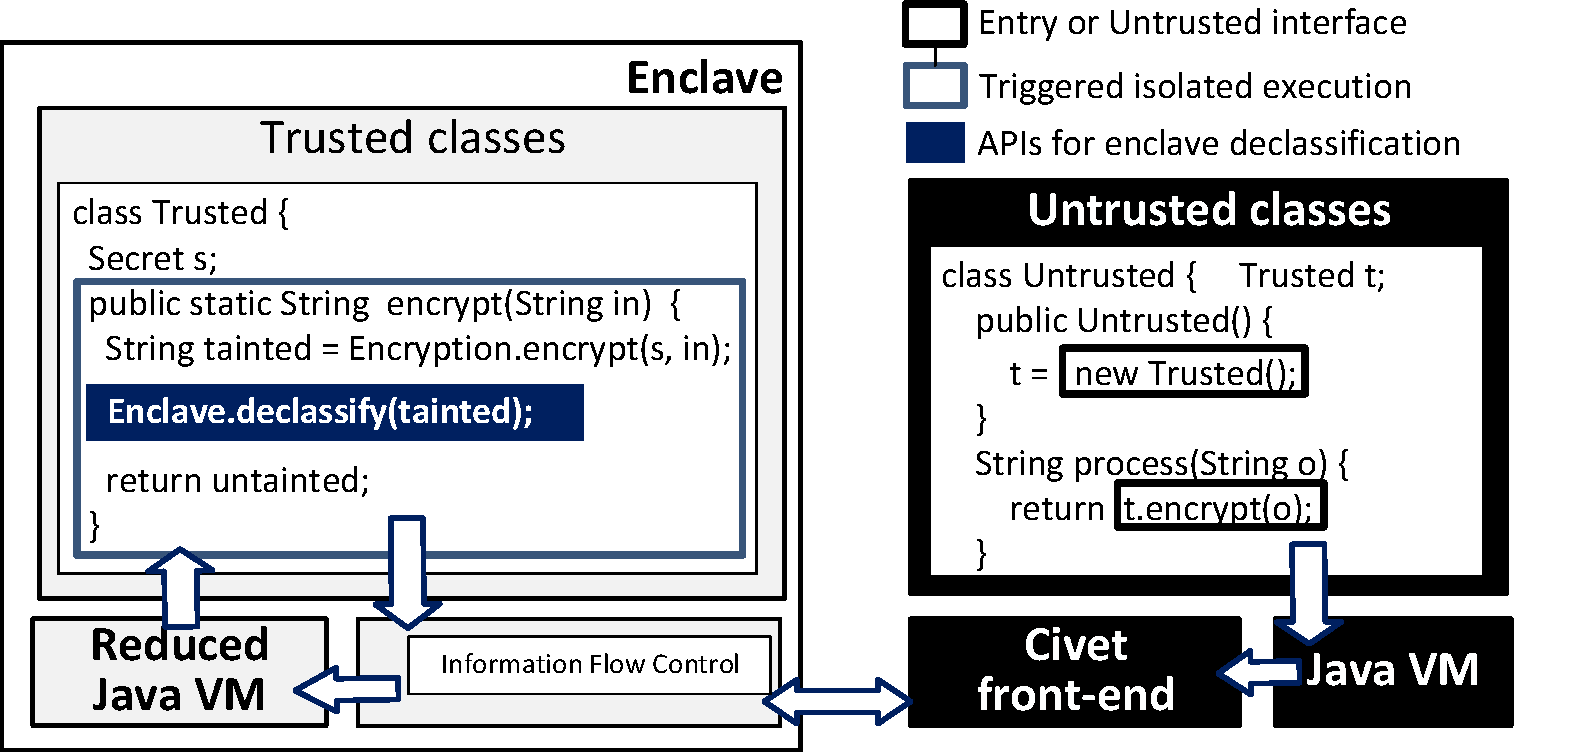
\includegraphics[width=1.0\linewidth]{declassify.pdf}
\footnotesize
\caption{How \sysname{} provides a declassifier API to declassify sensitive  data.
When the untrusted class ({\tt Untrusted}) from Figure ~\ref{fig:synthesis} now calls the {\tt encrypt} method of a trusted class ({\tt Trusted}),
\sysname{} automatically calls the {\tt encrypt} method inside enclave, and pass the {\tt byte[]} input.
Before returning, {\tt Trusted.encrypt} uses {\tt declassify()} to release the cipher generated and tainted  by {\tt cipher.doFinal()}.}
\label{fig:declassify}
\end{figure}

%Because the code running in enclave has access to complete address space, including the trusted as well as untrusted memory regions, it is easy for the trusted code to inadvertently undermine \sgx{} protection by writing secret information in the untrusted region. Further, leaking any information derived from or related to the secret may be used by the untrusted code to guess the value of secret information. For example, even in the presence of memory protection, sandboxing and virtualization, it is possible to recover the secret key used by crypto algorithms~\cite{kocher1996timing,osvik2006cache,weiss2012cache, zhang2012cross}. So, to ascertain the secrecy of the sensitive data, no information derived from the secret should exit enclave in plaintext.

%We use JAVA tool phosphor source and sink to taint provisioned data and control leakage
%\sysname{} leverages extensive research on information flow tracking and control in \java{} to harden the \sgx{} security. 

In the enclave, we implement source-to-sink taint tracking, using the open-source Phosphor library~\cite{phosphor}.
%\fixmedp{check this}
The programmer manually selects the classes containing secret data that take secret input from a remotely-provisioned source.
This taint is propagated to any new variables that result from explicit or implicit flows from a secret object.
The only way to remove taint from an object is to pass the object through a \sysname{} declassifier API,
which returns an untainted copy of the object.

%\fixmedp{Would be nice to have a simple example class with a label and declassifier in a figure, if space and time allow}

\sysname{} enforces the policy that only untained data may be returned from an enclave.
If tainted data is being returned, the system transparently encrypts the data and removes its taint before letting the data leave the enclave.
In the cases where a developer wants to return references to sensitive data, \sysname{} instead returns an opaque reference or, in the case of a literal, encrypts the return value.

%mFor tainted data, the developer may opt to either throw a runtime error, or, by default, to return an encrypted object instead.
%The en

% to taint the secret data when provisioned and propagate the taint to any new data generated as an explicit or implicit result of the secret data. We specify the enclave exit points as targets and enforce the policy that any tainted data must pass through a declassifier, that encrypts the data before egress. We only consider the provisioned data as security sensitive, as the enclave image is only integrity protected.

%Declassifier API: correct usage and scenarios
The \sysname{} framework provides a {\tt declassify(Object)} API that creates an untainted
copy of the object.  In practice, we expect this function to be used in conjunction with tests
on the returned data, or cryptographic functions to protect the data in transit across an untrusted channel.

Continuing our example from Figure~\ref{fig:synthesis}, in Figure~\ref{fig:declassify}, if the {\tt Untrusted} class wants to call the {\tt encrypt} method on the trusted object {\tt t}, \sysname{} front-end transparently passes the argument string {\tt o} to the enclave, and the corresponding {\tt encrypt} method is called in the enclave. The secret {\tt s} is tainted because it was provisioned from remote trusted server as shown in Figure ~\ref{fig:synthesis}. As a result, the call to method {\tt encrypt} of class {\tt Encryptor} taints the encrypted output string {\tt tainted}. If the developer had returned this {\tt tainted} variable, the \sysname{} information flow tracking would re-encrypt the ciphertext, and thus make the return value useless for the {\tt Untrusted} class. However, as the developer wants to return the ciphertext as is, she can declassify the {\tt tainted} string by passing it through the declassifier API to get an untainted version of the same object. Such untainted objects can be released from the enclave without further encryption.

%to let the application developer explicitly indicate that the argument object does not contain any secret information, and is safe to leave the enclave as is. For instance, if the enclave code encrypts a blob of data using the tainted secret provisioned key, the information flow will taint the encrypted data. However, because the encrypted data is safe to exit enclave if a perfectly secure encryption algorithm is used, the developer can explicitly mark the encrypted data as declassified. We note that the developers need to be extra careful while declassifying objects to inadvertently leaking secret information.

%Dealing with confidential code
%In order to protect the confidentiality of sensitive code,
%\sysname{} also allows classes themselves to be tainted.
%\sysname{} enforces a policy that any data returned from sensitive code is tainted, and the developer needs to explicitly declassify tainted output data to mitigate
%concerns around reverse-engineering the code based on brute-force probing of its outputs.
%Of course, the binary code itself is also not allowed to be copied out of the enclave.

% expose it to the untrusted world.
%The {\em code confidentiality} property of \sysname{} loads and executes encrypted classes from remote hosts to protect secret algorithm. We consider this provisioned code as equally security sensitive as provisioned data. ~

%\begin{table*}[t!b!]
\centering
  \begin{tabular}{p{0.05in} >{\raggedright\arraybackslash}p{2.05in} >{\raggedright\arraybackslash}p{4.4in}}
  \toprule
  \multicolumn{2}{l}{\it Security guarantees or features} & {\it The modeling approach applied by \sysname{}} \\
  \midrule
  \midrule
  \multicolumn{3}{l}{\bf Natively provided by the \sgx{} hardware (including the SDK):} \\
  \midrule
  & Isolating security-sensitive components &
  Asking developers to identify multi-level sensitivity, by marking the {\em entry classes}. Complete separation between isolated and untrusted classes.
  \\
  \midrule
  & Secure entry / exit of enclaves &
  Exporting public methods of isolated classes. Arguments are type-checked.
  \\
  \midrule
  & Integrity of the execution environment & 
  Packaging all supporting classes into a signed JAR.
  \\
  \midrule
  & Attestation \& secure provisioning & 
  Providing class {\tt Enclave}, to create secure channels and exchange attestation.
  \\
  \midrule
  \midrule
  \multicolumn{3}{l}{\bf Improvement from combining of \java{} language and the \sgx{} hardware protection:} \\
  \midrule
  & Memory safety \& control flow integrity &
  Naturally provided by \java{} language.
  \\
  \midrule
  & Reducing the enclave TCB &
  Automated partitioning based on class dependencies.
  \\
  \midrule
  & Preventing information flow leakage &
  Tracking information flow in trusted classes, only allow releasing the information if not tainted or declassified by developers.
  \\
  \midrule
  & Code confidentiality & Dynamically loading provisioned classes.
  \\
  \end{tabular}
  
\footnotesize
\caption{
The approaches applied by \sysname{} to model the security guarantees and features of the \sgx{} hardware, and to enhance the security by combining language and hardware protections.
}
\label{tab:features}
\end{table*}


%\input{Design of \jvm{} for SGX}
%\section{The \thelibos{} Architecture}


The \libos{} of \graphene{}, or 
\thelibos{},
is a single library to be loaded beneath a Linux application,
as a compatible layer between
Linux \linuxapis{} and \thehostabi{}.
The purpose of \thelibos{} is to reuse an unmodified Linux application
upon an incompatible host OS or hardware.
%to support compatible OS features.
%for exporting compatible features.
An unmodified Linux application is built with the assumption of running on a Linux kernel or equivalent.
A Linux kernel
has exported a set of idiosyncratic features and characteristics,
or {\bf personality},
which an unmodified Linux application depends on.
%In order to reuse an unmodified Linux application
%on an incompatible host,
\thelibos{} takes the role of reproducing the Linux personality,
and is equivalent to a guest Linux kernel
over various host options.
%using \thehostabi{} exported by the host OS and PAL.
%The purpose of \thelibos{}
%is to resue an unmodified Linux application,
%by combining with a PAL and a host OS to behave as an equivalence of a Linux kernel. 
%%which is developed upon the assumption of running on a Linux kernel or equivalent.
%The main purpose of \thelibos{} is to reproduce
%the idiosyncratic features and behaviors of Linux,
%or the {\bf Linux personality},
%to resurrect Linux applications upon incompatible
%host OSes or hardware.
\graphene{} develops \thelibos{} as an ELF dynamic library (i.e., \code{\tt libLinux.so}),
loadable and linkable by a PAL.
%to be loaded on a host by the corresponding PAL.
%at the beginning of a \picoproc{}.


A key component of \thelibos{}
is a Linux system call table, which redirects \linuxapis{} from a Linux application to functions in \thelibos{}.
%a key Linux kernel component applications. 
%that \thelibos{} implements is the Linux system call table.
%For Linux and similar OSes,
A system call table is a primary entry point of a Linux kernel.
Each entry of the system call table
points to the kernel implementation of a Linux API related with a \linuxapi{} number (e.g., \code{NR\_open}).
%and triggers in-kernel operations for servicing requests from applications.
%and defines the interaction between applications and kernel.
\graphene{} moves the Linux system call table into \thelibos{},
and implements a number of \linuxapi{} handlers in the user space.
%The system call table in \thelibos{} contains a number of \linuxapi{} handlers,
Each \linuxapi{} handler emulates
individual \linuxapi{} that \graphene{} supports;
\graphene{} develops each handler
based on either a known specification, % known by the Linux application developers,
mostly described by a Linux manpage~\cite{linux-man-syscall},
or bug-for-bug behaviors
observed in a real Linux kernel.
For example, \syscall{rt\_sigaction} is partially documented
in the corresponding Linux manpage, and \thelibos{} implements the \linuxapi{} by mimicking the Linux kernel.
\graphene{} grows the functionality of \thelibos{}
primarily by extending the guest-level Linux system call table
with more complete \linuxapi{} implementation.

%Otherwise, for a few \linuxapis{} whose behaviors
%are not clearly defined by the Linux manpages,
%such as \syscall{rt\_sigaction},
%the \linuxapi{} handlers mimic the bug-for-bug behaviors of an actual Linux kernel.
%A continuing goal in \graphene{} is
%to extend \thelibos{} with more complete \linuxapi{} handlers.


%grow the functionality of \thelibos{},
%by extending the system call table with more complete handlers.




%The development of \linuxapi{} handlers in \thelibos{}
%is equivalent to implementing the specifications described in the Linux man pages~\cite{linux-man-syscall},
%including the valid inputs to each \linuxapi{},
%as well as the expected outcome.


%\paragraph{Implementing Linux Personality.} 
%\fixmedp{Revisit the logical flow of these paragraphs}
\Thelibos{} currently implements \graphenesyscallnum{} \linuxapis{},
and demonstrates 
the sufficiency of running applications ranging from servers to command-line applications.
For reference,
a relatively recent Linux kernel contains more than three hundred \linuxapis{}, including a long tail of infrequently-used \linuxapis{}.
%upon \thehostabi{}. % to interact with the host.
%Among the whole Linux \linuxapi{} table,
%A Linux kernel exports a long tail of infrequently-used \linuxapis{}.
%For reference, the Linux \linuxversion{} kernel exports \linuxsyscallnum{} \linuxapis{}.
A study of the Linux \linuxapi{} usage~\cite{tsai16apistudy}
indicates that only forty \linuxapis{} are indispensable to every applications available in the Ubuntu official repositories.
%The study also shows that
In the meantime, more than a hundred \linuxapis{} are used by only a single application,
or no application at all.
The development of \thelibos{} begins with
implementing twelve basic \linuxapis{} needed for running a ``hello world'' application,
such as \syscall{read}, \syscall{write}, and \syscall{open},
and then gradually grows the count of \linuxapis{}.
%for each new application introduced to run on \graphene{}.
As the count of \linuxapis{} continues to grow,
each time \thelibos{} is tested against a new application, the number of \linuxapis{} that need to be added
has dropped.
%Based on the types of applications priorized in \graphene{}, including servers, command-line programs, and language runtimes, some \linuxapis{} to be more important %for reusing the applications
%than the others. % \linuxapis{}.
According to the usage of each \linuxapi{} in applications,
developers can prioritize the popular \linuxapis{}, over other \linuxapis{} that are either unpopular among applications, or only used by administrative tools such as \code{reboot} or \code{ifconfig}.
\thelibos{} demonstrates that
\thehostabi{} is sufficient for implementing
a significant subset of the Linux \linuxapis{} to run
a representative sample of applications.


%The current \thelibos{} implementation
%includes a set of high-valued Linux \linuxapis{} for the types of applications
%that \graphene{} has targeted,
%including servers, command-line programs, and runtimes.
%The remaning \linuxapis{} may require extending \thehostabi{} with more privileged abstractions,
%including administrative operations
%and host-specific features.
%\thelibos{} demonstrates that \thehostabi{} is sufficient
%for exporting the host abstractions, to support a representative sample of Linux applications.

%such as memory sharing, scheduler configuration, and NUMA (non-uniform memory architecture) support.


%Linux exports a very long tail of infrequently-used \linuxapis{}.
%applications.




%An analysis indicates roughly 100 additional calls that can be implemented
%with the existing \pal{} ABI and coordination framework, less than 10 administrative calls that will not make sense to expose to 
%an application, such as loading a kernel module or rebooting the system, and roughly 54 that will require 
%\pal{} extensions to meaningfully implement, such as controlling scheduling,
%NUMA placement, I/O privilege, and shared memory.
%In the last category of system calls, the degree to which actual host details should be exported versus emulated is debatable.

%We believe represent the most commonly used system calls.
%When an application requests a call or argument that {\tt libLinux.so} does not implement,
%the picoprocess exits with a distinct error message. 
%Each time we have tested \graphene{} with a new application, the number of extra system calls
%required has dropped---most recently we only added 4 calls
%(namely, epoll\_create, epoll\_wait, semget and semop)
%to support the Apache web server.
%Thus, we believe \graphene{} implements a representative sample of Linux calls.

%such as {\tt sched\_setparam}, which manipulates scheduler-specific
%parameters or 
%{\tt uselib}, which has been abandoned 
%in {\tt glibc} version 2 in favor of a user-space dynamic linker.
%We do not plan to implement administrative interfaces, such as {\tt reboot}.
%The growth in the set of supported system calls has been driven by 
%the requirements of new applications we use to exercise \graphene{}, and has been 
%slowing considerably over time.



\subsection{\Linuxapi{} redirection}


\thelibos{} transparently intercepts \linuxapis{} in a Linux application. In a Linux kernel, a \linuxapi{} interrupt handler is assigned
to trigger the kernel operations,
whenever the application executes
a ``\assembly{syscall}'' or ``\assembly{int \$80}'' instruction.
The handler
performs a context switch from the application to kernel,
and redirects \linuxapi{} arguments to the kernel routine which services the requested \linuxapi{}.
%based on a kernel convention agreed by applications and Linux kernels.
\thelibos{} intercepts the \linuxapis{}
from an unmodified Linux executable or library, and redirects
to the system call table implemented inside \thelibos{}.
%intercepts the \linuxapis{}
%in an executable or library binary, and redirect the \linuxapis{}
%to the \linuxapi{} handlers inside \thelibos{}.
%\thelibos{} implements the callback functions for a subset of the Linux \linuxapis{}.
%For reference, Linux kernel \linuxversion{}
%has defined \linuxsyscallnum{} \linuxapis{} in total.


In normal cases,
\thelibos{} can redirect \linuxapis{} from an unmodified Linux application
using a modified C library (\libc{}).
%from an unmodified Linux application.
Most Linux executables and libraries avoid invoking \linuxapis{} directly,
but use \libc{} functions as wrappers to \linuxapis{}.
%which internally execute ``\code{syscall}'' or ``\code{int \$80}'' instructions.
%an executable or library in Linux and similar OSes invokes \linuxapis{} through \libc{},
%instead of directly containing the \code{syscall} instructions.
%The \libc{}
%contains a large set of \linuxapi{} wrappers,
%which encapsulate direct \linuxapis{} to the kernel as functions.
For example, the \libc{} function \funcname{read} is a wrapper to the \syscall{read} \linuxapi{},
which internally executes
the \assembly{syscall} instruction.
% that bares the same name and definition.
By defualt, \thelibos{} uses a modified
{\bf GNU C library (\glibc{})}~\cite{glibc},
since \glibc{} is compatible against most Linux applications released by Ubuntu. % are compatible against \glibc{}.
%which is compatible against most of the Linux applications released for Ubuntu.
%Other \libc{} variants, ,
%which are either fully or partially compatible with \glibc{},
%can be also modified to redirect \linuxapis{} to \thelibos{}.
%are alternatives upon \thelibos{} as long as they are modified for .
\graphene{} can also use other \libc{} variants,
such as \projname{uClibc}~\cite{uclibc} and \projname{musl}~\cite{musl},
if the application requires less \libc{} functionality.
%\graphene{} demonstrates that 
%are also demonstrated
%to be acceptable alternatives,
%with slight modification for \linuxapi{} redirection.




\graphene{} restricts the modification in \glibc{}
to up to \gipclines{} lines of code.
The C source code in \glibc{} consistently uses a platform-independent macro,
%referenced a single macro called
\funcname{INLINE\_SYSCALL},
to invoke \linuxapis{} to the kernel.
%when it needs to invoke a \linuxapi{}.
\funcname{INLINE\_SYSCALL} contains a piece of assembly code
that copies \linuxapi{} number and arguments to registers,
and then uses \assembly{syscall} to enter a Linux kernel.
\graphene{} modifies \funcname{INLINE\_SYSCALL}
to redirect a \linuxapi{} to
an entry point of \thelibos{} called \funcname{syscalldb}.
\funcname{syscalldb} saves the current register state, similar to a context switch,
and then
calls the \linuxapi{} handler
indicated by the \linuxapi{} number.
%, to trigger operations inside \thelibos{}.
For assembly code in \glibc{},
\graphene{} replaces each \code{syscall} instruction with
a dynamic call to
\funcname{syscalldb}, given the address of \funcname{syscalldb} is dynamically determined.
Figure~\ref{fig:libos:syscall-redirection} summarizes the mechanism of \linuxapi{} redirection.
%to \thelibos{}.


\begin{figure}[t!]
\centering
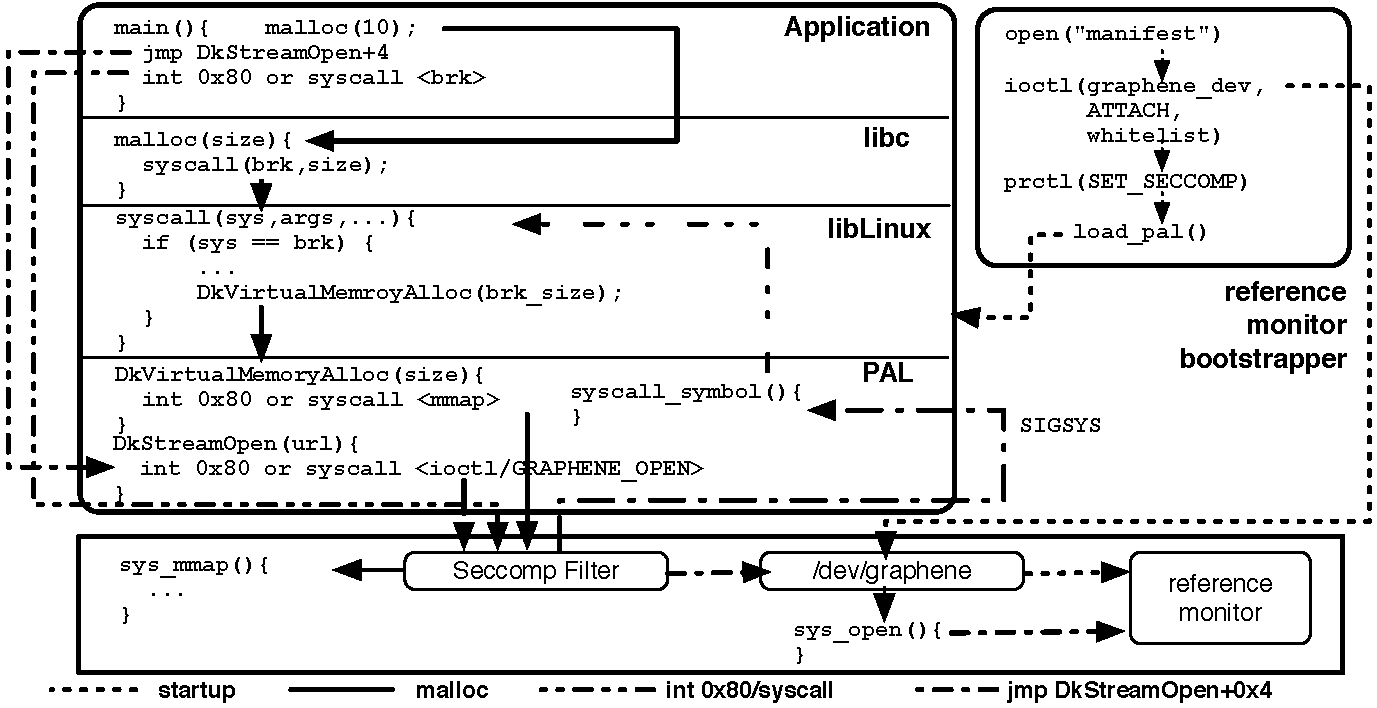
\includegraphics[width=\linewidth]{syscall-redirection.pdf}
\footnotesize
\caption{System call redirection for \thelibos{}.
In the normal case (first line of {\tt main}), {\tt malloc} is invoked causing the invocation of {\tt brk} ({\tt libLinux}) and {\tt mmap} in the \pal{}. In the second line, the application jumps to an address in \pal{}, which is permissible.
Files are accessed through {\tt ioctl} to {\tt /dev/graphene} and checked by reference monitor.
The third line invokes {\tt brk} with an {\tt int} instruction, which is redirected to the {\tt libLinux} function.}
\label{fig:libos:syscall-redirection}
\end{figure}


\graphene{} modifies several \glibc{} libraries with individual purposes,
%When using \graphene{}, an application must be deployed with the modified \libc{} libraries,
including \code{ld.so}, \code{libc.so}, \libpthread{}, and \libdl{}.
\Glibc{} partitions its code into separate libraries to reduce the binary sizes
loaded by each application.
%Despite that \glibc{} has partitioned its code into separate libraries,
\graphene{} only modifies the libraries which contains direct \linuxapis{} (i.e., \assembly{syscall} instructions).
%not every libraries of \glibc{} need to be modified for \linuxapi{} redirection.
%Only \code{libc.so}, \libpthread{}, and \libdl{} have included \code{syscall} instructions,
%and thus have to be modified for \graphene{}.
Other \libc{} libraries, such as \code{libm.so},
never directly invoke \linuxapis{} and only rely on 
existing \libc{} functions;
therefore, \graphene{} leaves \code{libm.so} and other similar \libc{} libraries unmodified.



\paragraph{Hard-coded \linuxapis{}.}
A static binary, or a platform-dependent application, may contain hard-coded \assembly{syscall} instructions
that cannot be redirected by a modified \libc{}.
Some application developers choose to statically link an executable against \libc{},
as a static binary with hard-coded \linuxapis{}. %\code{syscall} instructions.
Other application developers may program an application---usually a language runtime (e.g., go runtime) or system software (e.g., \projname{busybox})---with assembly code that directly invokes
platform-depenedent,
rare \linuxapis{} that are not wrapped by \libc{} functions.
%one of the \linuxapi{} wrappers in \libc{}, or \funcname{syscall}.
%As a result, a ELF binary may contain hard-coded \assembly{syscall} instructions.
%Either way leads to hard-coding \code{syscall} instructions in the ELF binaries.
Because modified \glibc{} does not redirect hard-coded \linuxapis{},
the \linuxapis{}
trigger context-switching into the host kernel,
causing security and compatibility issues as
exposing unauthorized, or unsynchronized host resources and states to the application.


As a solution,
\thelibos{} depends on host-level \linuxapi{} restriction to redirect hard-coded \linuxapis{}.
%to prevent \linuxapis{} from anywhere other than a PAL.
A direct \linuxapi{} traps into the host kernel,
unless the host has virtualized the interrupt handler to the \libos{}.
\graphene{} depends on each host to
detect unauthorized \linuxapis{} either from a wrong code location or with an unexpected \linuxapi{} number.
On Linux or a similar OS, the PAL can install a \linuxapi{} filter,
such as SECCOMP filter~\cite{seccomp}.
On some architecture, there are architectural limitation;
for example, SGX forbids \linuxapis{} inside an enclave and triggers an exception for an in-enclave \linuxapi{}.
%\code{syscall} instructions
%(e.g., SGX restriction).
%The details of the \linuxapi{} restriction mechanisms are discussed in
%\fixme{update labels}
%Section~\ref{sec:linux:syscall} and Section~\ref{sec:sgx:syscall}.
\thehostabi{} specifies that the host captures unauthorizes \linuxapis{}
and redirects to an exception handler (set up by \palcall{ExceptionSetHandler}).
%If a binary makes an illegal \linuxapi{},
%the host-level \linuxapi{} restriction will trigger an \code{ILLEGAL} exception
%at \thehostabi{},
%and thus the \linuxapi{} is redirected by an exception handler
%assigned by \thelibos{}.
The exception handler 
retrieves the \linuxapi{} number and arguments
from the saved context,
runs the \linuxapi{} handler,
and eventually pushes the return value back to the saved context. %\code{RAX} register.


Redirecting \linuxapis{} based on exceptions
can be expensive,
due to the overhead of context-switching between the host and guest.
Whenever an application invokes a direct \linuxapi{},
it traps into the host kernel, and then returns to the \libos{} to handle the \linuxapi{}.
Therefore, the process of redirecting a \linuxapi{} includes at least two times of context-switching, which can take up to microseconds.
To bypass the overhead,
\thelibos{} can 
rewrite the binary at run-time to redirect the hard-coded \linuxapis{};
%use {\bf binary translation} to modify the hard-coded \code{syscall} instructions;
\thelibos{} can
either scan-and-rewrites the whole binary at loading time,
or rewrites a single \assembly{SYSCALL} instruction in the exception handler.
%binary translation
%can be triggered when a host-level exception is raised
%for an illegal \linuxapi{},
%to optimize consecutive \linuxapi{} invocation at the same location.
%\thelibos{} can also perform a full scan in application binaries
%to spot and modify hard-code \code{syscall} instructions.
\graphene{} leaves the implementation of binary rewriting
as future work.



%\section{Automatic Partitioning of JAVA Applications}
\label{sec:partitioning}
\sysname{} reduces the TCB of a security critical 
application by automatically partitioning the 
application into trusted and untrusted parts. It is not 
easy for a novice developer to find the right 
partitioning boundary. As a result, the developer may 
include classes, which are not necessary for operation, 
in the trusted part. These extra classes may expose new 
attack vectors, reducing the security of the enclave. 
\sysname{} provides an enclave image utility to help 
the developer partition the code with minimum effort. 
The developer only needs to identify the classes that 
represent the secure objects.

The enclave image utility calculates the transitive 
closure of dependencies of the secure object classes.
The tool traverses all the imported classes by secure 
classes and marks them as secure too. The tool keeps 
traversing the newly added secure classes until there 
is no new class to be marked secure. It not only 
follows the user-defined classes but also the system 
classes to create a list of all the secure classes.

The utility then replaces the references of secure classes in the untrusted part with proxy stubs to make a remote method call instead of direct method invocation. The tool uses Phosphor information  flow tracking library to instrument the secure classes so that the information flow can be tracked at runtime as explained in Section ~\ref{sec:info-leak}. The output of the tool is an instrumented secure classes JAR and another JAR containing untrusted code with proxy stubs.

The enclave image tool then packages the Graphene LibOS, JVM, JNI, and the instrumented trusted JAR together, and generates the enclave object by cryptographically signing the package using its private key and \fixmebj{XX} algorithm. The untrusted JAR and the enclave object are deployed together in the cloud machine with \sgx{} capability. 

Thus, the automatic partition tool reduces the attack vectors exposed in the enclave, and removes the burden of the developer to create the partition boundary by finding the entry/exit points. This enforces a strict smallest possible TCB for the secure application.

%\papersection{Security isolation}
\label{sec:linux:security}

\issuedone{1.1.d}{Describe the security isolation story for Linux hosts}
\graphene{} separates OS features from security isolation.
This section explains the Linux host design for isolating mutually untrusting applications, with a reduced attack surface for protecting Linux kernels.
The discussion starts with the security guarantees and threat model, followed by the technical details of security isolation on a Linux host.



\papersubsection{Goals and threat model}

The security isolation model of \graphene{} ensures that mutually-untrusting applications cannot interfere with each other.
A goal of \graphene{} is to provide security isolation with comparable strength as
running applications in separate VMs.
When running two unrelated applications on the same machine,
the security requirement
of the OS involves not only blocking unauthorized access under normal circumstance,
but also preventing an application
from maliciously exploiting OS vulnerabilities to attack the other application.
Because a modern OS, such as Linux or \win{}, contains a rich of features and APIs,
it is difficult to eliminate OS vulnerabilities
or even just to verify whether an OS contains any vulnerabilities. 
A Linux container~\cite{lxc}
does provide a separate OS view for each application,
but still relies on the correctness of the whole Linux kernel to enforce security isolation.
On the other hand, a VM or a \libos{}
isolates the whole OS kernel or a part of the kernel in an unprivileged guest space
for each application.
The security isolation model prevents
any vulnerabilities inside the VM or the \libos{} from compromising the host kernel and other applications.



\graphene{} enforces security isolation %between applications
by separating 
backward-compatible OS features from security mechanisms.
A Linux kernel exports a wide range of system calls,
either as a legacy of previous kernels or as new programmability features. % of newer kernels.
By implementing OS features in a \libos{},
\graphene{} reduces the attack surface of a Linux kernel
to a small amount of system call corner cases.
%to implement \thehostabi{}.
%If a machine only runs applications in \graphene{},
%a Linux developer can try to carve out a minimal Linux kernel, containing only features needed by the Linux PAL.
A reduced attack surface
eliminates majority of execution paths inside a Linux kernel in which a malicious application can explore for vulnerabilities.
The complexity of Linux features and APIs exported by a \libos{} is unrelated with the attack surface of the host kernel,
unless the \libos{} asks for additional \hostapis{}.
A Linux developer can even carve out a minimal Linux kernel with only the features needed by the Linux PAL,
similar to shrinking a Linux kernel to a microkernel.
Otherwise, \graphene{} depends on the host security mechanisms to restrict a \libos{} from accessing unauthorized system calls and resources upon an unmodified Linux kernel.





The Linux PAL installs a {\bf system call filter} and a {\bf reference monitor}
for restricting the system calls, files, RPC streams, and network addresses
accessed by a \picoproc{}.
The Linux PAL requires \hostsyscallnum{} system calls in total
for implementing both required and optional \hostapis{}.
A system call filter, such as the Linux \seccomp{} filter~\cite{seccomp},
can restrict the system call access of an application
to only a small subset of all the system calls, with additional constraints on the parameters and optional flags permitted for each system call.
%The system call filter
%forbids an application from invoking any system calls
%that will interfere other \picoproc{} or increase the risk of exploitation in the host kernel.
A reference monitor further examines the arguments of permitted system calls to restrict the host resources accessed by an application, based on security policies configured in a manifest file~\cite{hunt07rethink}.
The system call filter and the reference monitor
significantly limit the ability of an untrusted \graphene{} \picoproc{} to interfere with the rest of the system,
preventing the risk of exposing any unknown vulnerabilities
on a kernel path never exercised by the system call footprint of \graphene{}.



\graphene{} contributes a multi-process security model 
based on a {\bf sandbox},
or a set of mutually-trusting \picoprocs{} running inside an isolated container.
The reference monitor permits picoprocesses within the same sandbox
to communicate over RPC streams,
allowing the \libos{} to share and coordinate any states
to create an unified OS view.
If two \picoprocs{} belong to different sandboxes,
the reference monitor will block any attempt of connecting RPC streams
between the \picoprocs{}
The access control over RPC streams
enforces an all-or-nothing security isolation model:
either two \picoprocs{} are in the same sandbox and share all the \libos{} states; or they are separated in two sandboxes and share nothing.
Even though the \libos{} instance can span its state across multiple \picoprocs{},
a host kernel needs not to examine the accesses to shared \libos{} states, but still enforces security isolation between sandboxes.




Files and network addresses
are the only host resources allowed to be shared across sandboxes,
using well-studied, explicit rules.
For sharing files, the reference monitor restricts the file access of a \picoproc{}
within a few host file or directories,
creating a restricted view of the local file system
(close to Plan 9's unionized file system views~\cite{pike90plan9}).
The file rules
in a manifest are similar to the policies of a {\bf AppArmor profile}~\cite{apparmor};
for each permitted file or directory,
a developer specifies the URI prefix and the permitted access type, either as read-only or readable-writable. %, within the target file or directory.
For sharing network addresses,
the reference monitor restricts a \picoproc{} from connecting through a local address or connecting to a remote address,
using {\bf iptables-like firewall rules}~\cite{iptablesman}.
Each network rule in a manifest
specifies the local or remote IP address and port range that a \picoproc{} is permitted to bind or connect a network socket.
The rules in a manifest file
specify a minimal list of files and network addresses that a \picoproc{} needs to access, and are largely based on existing security policies (e.g., AppArmor profiles, firewall rules).





\paragraph{Threat model (details).}
When running on a normal Linux host (without \sgx{} or other security hardware), \graphene{} assumes a trusted host kernel and reference monitor.
All the components inside the kernel space, including the \code{gipc} kernel module for bulk IPC, and the reference monitor,
are fully trusted by the other parts of the host kernel and the \graphene{} \picoprocs{}.
%which mediates all system calls with effects outside of a picoprocess's address space,
%such as file {\tt open} or network socket {\tt bind} or {\tt connect}.
On the other hand,
the host Linux kernel does not trust the \picoproc{}, including the Linux PAL, a \thelibos{} instance, \glibc{}, and the application.
The system call filter and reference monitor
initialized before an application starts running
defend the whole host kernel from malicious system calls invoked by a \picoproc{}.



All the components running within a \picoproc{}, including the Linux PAL, the \libos{} (\thelibos{}), \glibc{} libraries, and the application,
mutually trust each other. %, because all these components
%execute in the same guest address space.
Without internal sandboxing, the Linux PAL or \thelibos{}
cannot protect its internal states or control flows from an application.
Although some scenarios might require protecting the PAL or \thelibos{}
from the application,
\graphene{} only restricts the adversary
within a \picoproc{};
in other word, an adversary
only compromises the \libos{} in the same \picoproc{},
but can never interfere the host kernel 
or other unrelated \picoprocs{}.



For a multi-process application,
\graphene{} assumes that the \picoprocs{} 
%launched by the same application instance
running inside the same sandbox
trust each other and that all untrusted code run in sandboxed \picoprocs{}.
\graphene{} assumes the adversary can run arbitrary code inside
one or multiple \picoprocs within a sandbox.
The adversary can exploit any vulnerabilities in the \libos{}
or IPC protocol,
to propagate the attack to other \picoprocs{}.
\graphene{} ensures that
the adversary cannot interfere with any victim \picoprocs{}
in a separate sandbox.
A sandbox strictly isolates the coordination of \thelibos{} instances;
%if the only shared kernel abstractions are byte streams and files, 
the reference monitor ensures
that there is no writable intersection between sandboxes, so that
the adversary cannot interfere with any victim \picoprocs{}.


%%% The only processes allowed to run as standard kernel processes (non-\graphene{}) 
%%% are the reference monitor and
%%% system administration utilities that need more kernel interfaces than the \pal{} ABI provides.
%%% Ensuring that a collaborating picoprocess correctly implements
%%% some function (such as receiving a signal),
%%% as well as preventing exploitation of vulnerabilities in picoprocesses
%%% are beyond the scope of this work.

\graphene{} reduces the attack surface of the host Linux kernel, but does not change the trusted computing base; however, reducing the effective system call table size of a \picoproc{} does facilitate adoption of a smaller host kernel.
This thesis leaves the creation of a smaller host kernel for future work.

\papersubsection{System call restriction}
\label{sec:linux:security:syscall-restriction}


\graphene{} reduces the host ABI to \palcallnum{} calls
and the Linux system call footprint to \hostsyscallnum{} system calls.
To reduce the effective attack surface to a Linux host,
the Linux host restricts a \picoproc{} from accessing any system calls that are not part of the ordinary footprint of a Linux PAL.
The system call restriction on Linux focuses on blocking most of the system calls
that interferes with other processes.
The remaining permitted system calls with external effects are checked by 
the reference monitor (see Section~\ref{sec:linux:security:ref-monitor}).
 
%% dp: Meh
%%% Any picoprocess implementation 
%%% must restrict access to the host system call table,
%%% generally by blocking system calls in the host kernel~\cite{porter11drawbridge}
%%% or using {\tt ptrace}~\cite{xax}.


%The \pal{} is a host-provided library which implements \palcalls{} generic kernel ABIs,
%implemented using 
%These native system calls include {\tt ioctl} with 5 opcodes exclusively used by \graphene{} kernel extensions.

%This section describes how we adapt recent Linux sandboxing techniques 
%to \graphene{}.


%all allowed system calls with potentially external effects.

%%% For instance, an attempt to open a file will be checked by the reference monitor
%%% to see if the file is included in the sandbox definition, specified in the manifest
%%% with required permissions.
%%% Once the file handle is open, the \pal{} is then allowed to issue an {\tt mmap} or {\tt read}
%%% on the handle, as this operation can only affect the picoprocess address space
%%% or  file, which was already checked.

%Because the \pal{} is in the same address space as the application code, it is not
%trusted to enforce any security policies, and our threat model assumes that
%the \pal{} can be compromised by the adversary.
%Thus, the host kernel 
%only permits system calls that appear in the \pal{}'s source code and, through the reference monitor, further inspects calls that can have external effects.

%\begin{figure}[t!]
%\centering
%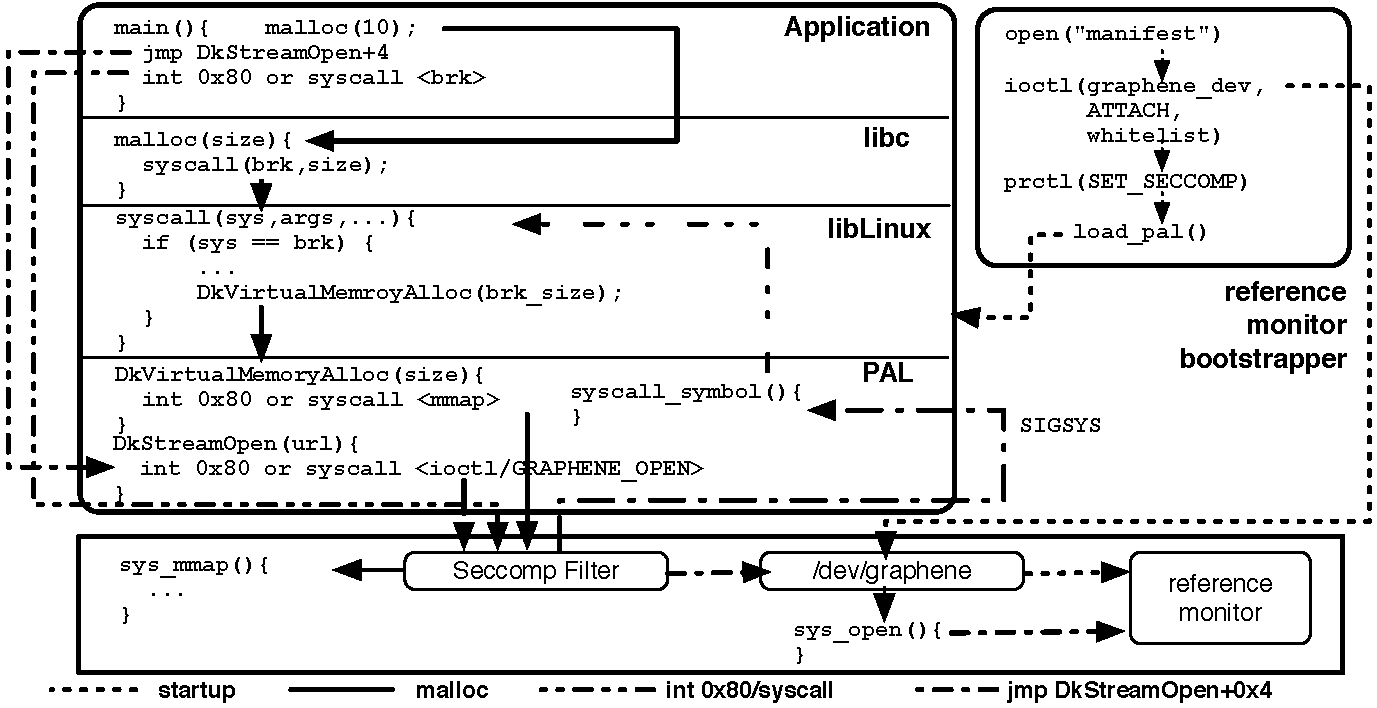
\includegraphics[width=\linewidth]{syscall-restriction.pdf}
%\footnotesize
%\caption[System call restriction approach in sysname{}]
%{System call restriction approach. The reference monitor loads policies into the LSM at startup.  A \graphene{} application requests OS services in three different ways. 
%In the normal case (first line of {\tt main}), {\tt malloc} is invoked causing the invocation of {\tt brk} ({\tt libLinux}) and {\tt mmap} in the \pal{}. In the second line, the application jumps to an address in \pal{}, which is permissible.
%Files are accessed through {\tt ioctl} to {\tt /dev/graphene} and checked by reference monitor.
%The third line invokes {\tt brk} with an {\tt int} instruction, which is redirected to the {\tt libLinux} function.}
%\label{fig:graphene:syscall-restriction}
%\end{figure}



\issuedone{1.3.d}{Extend the discussion of \seccomp{} filter}
\graphene{} restricts the host system calls 
using a \seccomp{} %(SECure COMPuting)
filter~\cite{seccomp}, a feature introduced in Linux 2.6.12.
% a recent Linux system call filtering mechanism, called 
A \seccomp{} filter allows a Linux process to install an immutable Berkeley Packet Filter (BPF) program
that specifies allowed system calls, as well as specifies
the consequence of invoking certain system calls, such as creating a \code{ptrace} event or raising a \code{SIGSYS} signal.
The BPF grammar is rich enough to filter scalar argument values,
such as only permitting specific opcodes for \syscall{ioctl},
as well as filter certain register values, such as blocking system calls from program counters (i.e., \code{RIP} register values) outside of the Linux PAL.
%This feature is particularly salient in the case of {\tt ioctl},
%where the \pal{} uses 5 out of over 400 opcodes for our bulk IPC module and sandbox creation;
%our BPF rules will block any other {\tt ioctl} opcode.
The current \seccomp{} filter installed by the Linux PAL contains \seccomplines{} lines of straightforward BPF macros.  %Experiments show that adding more precise argument checks has no significant impact on system call latency.
Once a \seccomp{} filter is installed in a process,
the filter intermediates
every system calls from the process and its future children, and guarantees the processes can never bypass the restriction.
The Linux PAL uses \code{SIGSYS} signals to capture rejected system calls,
and can either terminate the whole application or
redirect the system call to \thelibos{}.
The consecutive steps of system call redirection are described in Section~\ref{sec:libos:syscall-redirection}.



Developing a \seccomp{} filter presents several technical challenges.
First, a filter must restrict consecutive \picoprocs{}
to install a new filter the reverts the system call restriction.
%A \seccomp{} filter is installed using the \syscall{prctl} system call, so
Blocking the \syscall{prctl} system call in a \seccomp{} filter will prevent further installation of \seccomp{} filters.
Second, the BPF grammar can only filter certain values or ranges of a register.
The filter needs to
ensure that only the Linux PAL can invoke system calls;
however,
for satisfying the dynamic loading behavior of \thehostabi{},
the Linux PAL
is built as a shared library loaded at an address randomized by the Linux ASLR (Address Space Layout Randomization) feature.
If a filter only permits a specific range of program counters,
a child \picoproc{}
will load the Linux PAL at another randomized address,
and the inherited filter will restrict the child \picoproc{} to invoke any system calls.
The Linux PAL introduces a small, initial loader
loaded at a fixed address
within each \picoproc{} and permitted to invoke system calls.
Finally, a \seccomp{} filter
cannot check a string argument, such as a file path for \syscall{open} or a network address for \syscall{bind}.
Checking a string argument requires
involves reading user memory of unknown sizes and string comparison, and the BPF grammar only allows checking an argument arithmetically.
Filtering permitted file paths and network addresses
must rely on a trusted reference monitor (see Section~\ref{sec:linux:security:ref-monitor}).
%In order to avoid the overhead of trapping to the reference monitor on 
%every use of {\tt open}, {\tt stat}, {\tt bind} or {\tt connect} system calls, we instead 
%force picoprocess to only use {\tt ioctl} system call to \graphene{} special device ({\tt /dev/graphene}) as alternative interface these system calls. Direct access to these system calls are banned by seccomp filter.
%extend AppArmor~\cite{apparmor} 
%to enforce file system isolation in the kernel.



The \seccomp{} filter blocks  unauthorized system calls
from anywhere inside a \picoproc{}.
Even if none of the application binaries contains any \assembly{syscall} or \assembly{int \$80} instruction,
a piece of malicious application code can always bypass the Linux PAL
to invoke unauthorized system calls.
The application code can simply
jump to a \assembly{syscall} instruction inside the Linux PAL,
or corrupt a returned address on the current stack to launch a ROP (return-oriented programming) attack.
Even if the Linux PAL is hidden or isolated from the application,
an adversary can always leverage a gadget, a byte sequence that resembles the target instruction, within an executable or a library.
Therefore, the \seccomp{} enforces both program-counter-based 
and argument-based restrictions
to block unauthorized system calls from both the Linux PAL and the rest of \picoproc{}.


%In order to reduce the impact of bugs in the reference monitor,
%the reference monitor itself runs with a \seccomp{} filter, blocking unexpected system calls.


\paragraph{Security implications.}
Using an existing system call restriction mechanism like \seccomp{},
\graphene{} limits the ability of an untrusted application to attack a Linux kernel.
Ideally, since \thelibos{} only requires \thehostabi{},
\graphene{} can adopt a modified Linux kernel
that only exports \palcallnum{} \hostapis{} to each \picoproc{}.
%However, as a usability feature, \graphene{} runs \graphene{} on an unmodified Linux kernel using a Linux PAL to translate among host interfaces.
The \seccomp{} filter instead isolates a \picoproc{} on an unmodified Linux kernel,
with a reduced attack surface 
comparable to only exporting \thehostabi{}.
%The filter only permits \hostsyscallnum{} system calls with specific flags and opcodes
%required by the Linux PAL.
According to the principle of least privilege,
each component or layer in a system should only be granted access to a minimal amount of resources or abstractions
required for performing the expected tasks.
The \seccomp{} filter only permits
a minimal amount of system calls with specific flags and opcodes
required by the Linux PAL,
so an untrusted application
can only trigger
a limited amount of execution paths inside the host Linux kernel.
\graphene{} limits
the ability of an untrusted application to explore
known and unknown vulnerabilities
on any kernel execution paths for servicing one of the blocked system calls.



Although a regular Linux process can also leverage a \seccomp{} filter,
\graphene{} makes a major contribution
to reduce the system call footprint of any large-scale application
to a fixed, small system call profile.
Analysis %of applications and libraries
%in the official Ubuntu repositories
shows that the system call  footprint of a large-scale application such as Apache or MySQL can contain more than 100 system calls.
Since \thelibos{} has absorbed the Linux system call table,
running Apache, MySQL, or any other application in \graphene{} leads to at most \hostsyscallnum{} host system calls.
As a system
running a wide range of applications
can exposes a different partial view of the system call table to each application,
\graphene{}
has a static system call profile for all applications,
allowing OS developers to focus
on testing or analyzing a small portion of execution paths and corner cases
of a Linux kernel.
\citet{sun15unpredictability}
proposes sandboxing an uncertain, potentially-malicious application
in \graphene{}
with an unpredictable \thelibos{} implementation.







\paragraph{Static binaries.}
Besides security purposes,
a \seccomp{} filter provides a compatibility feature
for redirecting hard-coded system calls
in a statically-linked application binary.
\graphene{} leverages the \seccomp{} filter to redirect these leaked system calls
back to \thelibos{}. 
The filter contains BPF rules to check if the program counters
invoking the system calls
are parts of the Linux PAL.
The filter blocks system call invoked outside of the Linux PAL
and delivers a \code{SIGSYS} signal
to the PAL signal handler for redirecting the system calls to \thelibos{}.



\papersubsection{Reference monitor}
\label{sec:linux:security:ref-monitor}

The reference monitor on a Linux host
checks the arguments of host system calls for referencing any sharable host resources.
A host system call like \syscall{open}, \syscall{connect}, or \syscall{bind}
specifies a file system path or a network address
for opening a file or network stream and cannot be filtered by a \seccomp{} filter.
The host kernel trusts the reference monitor
to only permit
a list of sharable resources in a \picoproc{},
based on
rules in a manifest file.
Once the reference monitor has permitted the creation of a file or network stream,
consecutive operations on the stream
such as reading or writing data can be trusted
as long as being mediated by one of the permitted system calls.


\begin{figure}
\centering
\begin{lstlisting}
loader.exec = file:/usr/sbin/apache2        # allow loading executable 
loader.preload_libs = file:/graphene/libLinux.so    # loading libLinux
fs.allow_ro.libc = file:/graphene/libc/     # loading modified libc
fs.allow_ro.mods = file:/usr/lib/apache2/modules/   # loading modules
fs.allow_ro.cond = file:/etc/apache2/       # reading configuration
fs.allow_rw.logs = file:/var/log/apache2/   # writing to logs
fs.allow_ro.http_docs = file:/var/www/      # reading website files
net.allow_bind.httpd = 0.0.0.0:80           # binding to local port 80
net.allow_conn.any = 0.0.0.0:1-65535        # allow any connection
\end{lstlisting}
\caption{A example of a manifest file, containing security rules for the reference monitor to permit accessing sharable resources. The manifest file is for running a Apache http server (without php and other language engines).}
\label{fig:linux:manifest-example}
\end{figure}


The reference monitor enforces simple, white-listing rules
based on security mechanisms
already familiarized by users and developers.
Figure~\ref{fig:linux:manifest-example} shows an example of resource access rules
in a manifest.
First, a manifest lists
the URI prefixes of permitted files or directories
of an application,
similar to an AppArmor profile.
The executable (\code{loader.exec}) and the preloaded \libos{} binaries (\code{loader.preload\_libs})
are permitted for read-only access by default.
The reference monitor
simply compares file URIs against each permitted URI prefix
and checks the access types;
unlike many existing security mechanisms in Linux and similar OSes, such as permission bits, Access Control Lists (ACLs), and SELinux labels,
the reference monitor does not retrieve
security policies from file metadata, but obtains the manifest from an out-of-band channel.


Manifest-based security
simplifies the inspection, authentication, and population
of security policies.
An Android application is deployed with a similar manifest,
listing the accessed files and other resources,
which users approve when installing the application.
Developers can authenticate a security policy by signing the content of a manifest.
Moreover, to run an application, a user can choose among multiple manifest files
with different levels of security privileges.



Network rules in a manifest are similar to {\bf iptables firewall rules} for defending a server or a desktop machine.
A network rule specifies a local or remote address
that the application is permitted to bind or connect a network stream.
A local or remote address
can be an IPv4 or IPv6 address (possible to specify an ``any'' address, i.e., \code{0.0.0.0} or \code{[::1]}), combined with a specific port number or range.
When an application creates a network stream,
the reference monitor checks whether the local and remote addresses
match one of the network rules.







%is implemented using {\tt ioctl} system call to a special device {\tt /dev/graphene}.
%A picoprocess is restricted by seccomp filter~\cite{seccomp} to use any {\tt open} or socket {\tt connect} and {\tt bind} system calls.
%It must use the \graphene{} special device to open or create streams,
%so the file paths or network addresses can be checked against the sandbox rules.
%The kernel module as the driver of the \graphene{} special device can coexist with any LSM such as \emph{AppArmor} or \emph{SELinux}.

The reference monitor on a Linux host
is implemented as a Linux Security Module (LSM) extended from the existing AppArmor module.
AppArmor is the default LSM of most Linux distributions,
and a Linux kernel disallows multiple LSMs (e.g., AppArmor, SELinux) to be effective simultaneously.
\graphene{} instruments
a few security hooks of the AppArmor, to add checks for file system paths
and network addresses.
The security checks of the reference monitor are stackable with other host security mechanisms.
For example, if a manifest lists a root-privileged file and the \graphene{} application runs in a unprivileged process,
existing security checks in a Linux kernel
still blocks the file access even though the reference monitor permits the access.
The drawback of the implementation
is that \graphene{} must run on a modified Linux kernel.
Linux kernels do not support loading LSM as a dynamic kernel module.
\graphene{} only replaces
the AppArmor LSM in a Linux kernel; the rest of the Linux kernel remains unchanged.


A trusted security loader initializes the reference monitor
when launching an application in \graphene{}.
When a user launches an application in \graphene{} from the command line,
the first \picoproc{} begins in a new sandbox.
The security loader
reads the manifest file given by the user,
and submits the sandbox rules to the reference monitor.
The reference monitor exports a miscellaneous device called \code{/dev/graphene}
for the security loader to submit sandbox rules using the \syscall{ioctl} system call.
Once the reference monitor
starts a \picoproc{} in a sandbox, neither the first \picoproc{} nor any consecutive \picoprocs{} spawned in the sandbox can ever escape the sandbox or drop the restrictions on certain resources.


\paragraph{Alternative approaches.}
Other approaches can implement the reference monitor without modifying a Linux kernel, with a trade-off of performance or development simplicity.
An approach is to implement the reference monitor as a trusted process receiving \code{ptrace} events from \graphene{} \picoprocs{}.
Using the \syscall{ptrace} system call, this reference monitor can retrieve user memory from the monitored \picoprocs{},
and block the system calls which request for unpermitted resources.
Unfortunately, intercepting every system calls with \code{ptrace} events introduces significant overhead to \hostapis{};
thus, this approach is not ideal for isolating \graphene{} applications on a Linux host.


Another approach is to translate the resource rules in a manifest file
to AppArmor or iptables rules.
As explained in previous paragraph, the file and network rules in a manifest file are similar to the file lists in an AppArmor profile and the firewall rules enforced by iptables.
Instead of implementing a \graphene{}-specific reference monitor,
\graphene{} can convert a manifest file, either statically or dynamically,
to security rules recognized by AppArmor and iptables.
This approach requires no modification
in a Linux kernel, and can benefit from
existing optimizations of AppArmor and iptable. %these security mechanisms.
\graphene{} leaves the integration with AppArmor and iptables for future work.




\paragraph{Dynamic process-specific isolation.}
A child \picoproc{} may either inherit its parent's sandbox, 
or start in a new sandbox,
by either specifying a flag to \palcall{ProcessCreate} or calling the sandboxing \hostapi{}, \palcall{SandboxSetPolicy}.
A new sandbox may obtain a subset of the original file system view,
but can never request access to new regions of the 
host file system. 
%The restrictive policy enforced on the child will be written in a new manifest file generated by the parent, and the policy will be checked by the reference monitor.
If a child \picoproc{} voluntarily moves itself to a new sandbox
using \palcall{SandboxSetPolicy},
the Linux PAL issue another \syscall{ioctl} call to \code{/dev/graphene}
to dynamically detach
the \picoproc{}
from the parent's sandbox and update sandbox rules. The reference monitor
closes existing RPC streams and prevents RPC stream creation 
across sandboxes.
%among picoprocesses
%that are not in the same sandbox.
%and restricts external connections to remote URIs according to firewall rules in the manifest.
When a process detaches from a sandbox,
the reference monitor effectively splits the original sandbox
by closing any RPC streams that could bridge the two sandboxes.


\begin{comment}
We hasten to note that program counter filtering
is only provided for backwards compatibility, not security.
An attacker can compromise the \pal{}, so system policies are enforced
externally by the reference monitor.


Dynamically redirecting system calls to {\tt libLinux} is 
less efficient than dynamically linking against
the \graphene{} libc or statically compiling {\tt libLinux} into the application.
The overhead of dynamic redirection comes from 
transferring control to the kernel, then back to 
the \pal{}, and then to {\tt libLinux}.
We leave exploration of more efficient alternatives for future work,
such as redirecting the hardware system call table to {\tt libLinux}
on a host system like Dune~\cite{belay12dune},
or dynamically rewriting parts of the static binary~\cite{hunt99detours}.
\end{comment}

%\paragraph{Example.}
%Figure~\ref{fig:graphene:syscall-restriction} illustrates three possible situations. 
%%% An unmodified Linux application is dynamically linked against the 
%%% \graphene{} {\tt libc}, 
%%% which then dynamically links its system calls from {\tt libLinux},
%%% which in turn links in the host kernel ABI from the \pal{}.
%%% The application requests OS functionality in three ways.
%An unmodified application first invokes the {\tt libc} function {\tt malloc}, which issues 
%a {\tt brk} system call to {\tt libLinux}, which requests memory 
%from the host via a {\tt Dk\-Virtual\-Memory\-Alloc} \pal{} call,
%which ultimately issues an {\tt mmap} host system call.
%The {\tt mmap} host system call is allowed by seccomp because it only 
%affects the picoprocess's address space.
%The second line of the application jumps to the \pal{} instruction that issues
%an {\tt open} system call.
%From a security perspective, this is permissible,
%as it is isomorphic to \pal{} functionality.
%In practice, this could cause
%corruption of {\tt libLinux} or application data structures,
%but the only harm is to the application itself. 
%Because this system call involves the file system, the reference monitor LSM first checks if the file to be opened is included in the sandbox definition (manifest) before allowing  the {\tt open} system call in the kernel.  
%Finally, the application uses inline assembly to issue a {\tt brk} system call;
%%in an attempt to obtain I/O port privilege; 
%because this system call was not issued by the \pal{},
%seccomp will redirect this call back to the \pal{},
%which then calls the {\tt libLinux} implementation.


Sandbox creation in \graphene{} can provide
more options than virtualization, to reflect the security policy of applications at any timing,
in the granularity of picoprocess. 
A picoprocess can voluntarily detach itself from the current sandbox, dropping its privileges,
after finishing security-sensitive operations.
If a picoprocess decides one of its children is not trustworthy, it may also start the child under a restricted manifest,
or promptly shut down RPC streams to stop sharing OS states.
The picoprocess that moves to a separate sandbox will have a restrictive view of the filesystem, and no coordination with the previous sandboxes.
Section~\ref{sec:eval:graphene} describes an experiment that improves security isolation of Apache http server without sacrificing functionality.



%We add a \pal{} call which
%permits a picoprocess to request that it be moved into a new sandbox.
%This call, as well as file system path checks, are implemented
%as extensions to the  AppArmor LSM~\cite{apparmor}.
%%We modify \sandboxmodlines{} lines in the
%%to implement this call,
%The new sandbox call closes any open stream handles that cross sandbox boundaries;
%mediate path lookups;
%and create a new broadcast stream for multi-process
% coordination (\S\ref{sec:graphene:namespaces:blocks}).
%%The reference monitor also interposes on this call so that it can 
%%mediate future stream creation.

%To securely apply seccomp filtering we leveraged the fact that all
%\graphene{} processes have the same parent and also the new
%{\tt NO\_NEW\_PRIVS} bit introduced for Linux processes starting kernel
%version 3.5. This bit can be set by any process, is inherited across
%{\tt fork}, {\tt clone}, and {\tt execve}, and cannot be unset by
%children processes. Thus, we set the {\tt NO\_NEW\_PRIVS} bit in the initial
%\graphene{} process and apply seccomp filters allowing only system calls
%with corresponding functions in the \pal{}. As a result all \graphene{}
%processes will inherit the filters and cannot relax or bypass it.



%which reduces the kernel
%system call API surface to user-level processes. This mechanism allows
%a process to specify a whitelist filter for system calls, which is
%implemented as a Berkeley Packet Filter (BPF) program. The invocation
%of a disallowed system call causes the application to throw a {\tt SIGSYS}
%signal, which can be caught by a registered handler provided by the
%application. In \graphene{} we registered this handler at the \pal{}.


%\graphene{} applications rely on an OS loaded as a library to request
%system services. As most of traditional applications, \graphene{}
%processes do not normally issue system calls directly: they invoke
%wrapper functions from a \graphene{}-compliant version of libc, which
%allows for portability, security (parameters are limited and checked)
%and easiness of programming. However, while standard libc functions
%directly invoke the kernel system call themselves, our modified
%version of libc wrappers invoke functions from another library which
%represents the OS, libLinux (Figure \ref{fig:graphene:syscall-restriction}). A
%\graphene{} application can access all necessary system functionality
%through libLinux, which invokes corresponding system call functions at
%the \pal{}, also loaded as a library with a
%\graphene{} process. The \pal{} is the layer responsible for directly
%invoking system calls at the kernel. As discussed in \S\ref{sec:graphene:impl} the \pal{} provides \graphene{} applications with a
%subset of the kernel system call interface.\graphene{} applications rely
%on an OS loaded as a library to request system services.
%
%Even though we expect most of \graphene{} applications to leverage libc
%wrappers, we need to address applications that need to invoke system
%calls directly. Applications might need to bypass a library such as
%libc because some needed wrappers are not provided (there are no
%wrappers in libc for module and NUMA related system calls), or the
%wrapper does not meet the programmer’s needs. \graphene{} applications
%that need to perform direct invocation of system calls run unmodified
%as long as the system calls invoked are provided by the libos{l{}. We
%do not consider this a security violation; even though the application
%would be risking not functioning according to the libosaradigm for
%bypassing the \pal{}, all potential damage would be confined in the
%misbehaving application itself.  However, we do not allow the direct
%invocation of a system call that does not have a corresponding
%function in the libosnd \pal{}. In Figure \ref{fig:graphene:syscall-restriction}
%we illustrate these three situations. We have a \graphene{} application
%loaded with three libraries: a \graphene{}-compliant libc, libLinux
%representing the library OS with functions for a selected number of
%system calls, and the \pal{} which actually invokes host kernel system
%calls. The illustrated application requests three different types of
%OS functionality. It first invokes a function from libc, then it
%directly invokes a system call whose functionality is provided by the
%\pal{}, and third it attempts to directly invoke a system call not
%present in the \pal{}, which is not allowed by \graphene{}.

%We enforce system call restriction by leveraging seccomp Linux system
%call filtering mechanism~\cite{seccomp}, which reduces the kernel
%system call API surface to user-level processes. This mechanism allows
%a process to specify a whitelist filter for system calls, which is
%implemented as a Berkeley Packet Filter (BPF) program. The invocation
%of a disallowed system call causes the application to throw a {\tt SIGSYS}
%signal, which can be caught by a registered handler provided by the
%application. In \graphene{} we registered this handler at the \pal{}.
%
%To securely apply seccomp filtering we leveraged the fact that all
%\graphene{} processes have the same parent and also the new
%{\tt NO\_NEW\_PRIVS} bit introduced for Linux processes starting kernel
%version 3.5. This bit can be set by any process, is inherited across
%{\tt fork}, {\tt clone}, and {\tt execve}, and cannot be unset by
%children processes. Thus, we set the {\tt NO\_NEW\_PRIVS} bit in the initial
%\graphene{} process and apply seccomp filters allowing only system calls
%with corresponding functions in the \pal{}. As a result all \graphene{}
%processes will inherit the filters and cannot relax or bypass it.


%\begin{figure}
%\begin{centering}
%\includegraphics[width=2.0in\textwidth]{figures/syscall_restriction.png}
%\footnotesize
%\caption{System call restriction approach. \graphene{} application requesting OS services. The {\tt printf} function is handled by a wrapper function at our modified version of libc., which invoked a corresponding syscall function at libLinux, the library OS.This function invokes a system call function at the \pal{}, which actually invokes kernel system calls. The application also directly invokes two system calls and the last invocation is prohibited.
%\label{fig:syscall_restriction}
%\end{centering}
%\end{figure}

%\end{comment}

%\papersection{Seamless Provisioning of Secure Objects and Classes}
\label{sec:provisioning}

%\section{Framework Implementation}
\label{sec:implementation}

In this section we describe the design of \sysname{}.
\sysname{} adds language support in \java{} virtual machines to
create and execute partitioned applications in enclaves.

\subsection{Partitioned \java{} Execution}

To executed partitioned applications,
\sysname{} creates two worlds of \java{} execution,
one in an enclave and one outside the enclave,
to execute code at different security levels.
Each world contains an individual \java{} vM.
We allow only classes that are part of a signed enclave images to
be executed inside the enclave,
and all the other classes of the application
must run outside the enclave and access the secured classes through
an interface exported by the enclave.

Using \java{} language to implement enclaves
has the benefit of minimizing the development or porting cost.
Consider partitioning a native application for enclaves.
There are two primary sources of development or porting cost:
Separating the security-sensitive code from all the remaining code,
and designing the interface between the two.
%\java{} classes have huge advantage on fulfilling both goals
%with minimal works, for two reasons:
\java{} classes are well modularized and are natural granularity for partitioning.
Public methods can be exported as
enclave interfaces, with proper type-checking of arguments.

%\sysname{} allows \java{} applications
%to easily model enclave support as part of the language,
%without the awareness of the native interface to architecture.
%To reflect this concept, we have implemented two key principles in the language support:
%\begin{compactenum}
\sysname{} models each enclave as an object,
both inside and outside the enclave.
The object is used to access enclave information and features,
such as retrieving security attestation.
Instantiating and interfacing with the isolated classes
in enclaves is transparent to the untrusted part of application,
except the first instantiation.

%For the untrusted side of an application, both the enclave itself and
%the classes isolated in the enclaves
%are encapsulated as black boxes, to which the application
%can request for isolated execution seamlessly.
%These objects can be passed as parameters to other methods,
%or even overrode to extend their functionalities.

\begin{figure}[t!]
\vspace{-0.1in}
\centering
\includegraphics[width=3in]{civet-structure.pdf}
\vspace{-10pt}
\caption{\sysname{} framework overview. \sysname{} creates two worlds for an partitioned \java{} application, each with an individual JVM. The JVM in the enclave is ported using Graphene library OS. Untrusted classes can invoke methods of trusted classes through proxy objects, which will transparently access the enclave interface, through serialization and deserialization over an ring buffer accessed by both untrusted JVM and trust JVM. }
\label{fig:overview}
\end{figure}

\paragraph{Framework overview.} Figure ~\ref{fig:overview} shows the design and 
components of ~\sysname{} infrastructure.
All supporting classes to be isolated in the enclave
are packed into a JAR package --- an enclave image ---
and signed using a key given by the developers.
The untrusted side of the application initializes the enclave
using the enclave image JAR,
and starts to instantiate objects inside the enclave.
For each objects in the enclave, \sysname{} create a {\em proxy object} outside the enclave,
to access the interface exported from the enclave.
%and to represent the isolated objects to the rest of world.

The JVM running inside the enclave is a \jvmname{} VM
ported with the libOS-based programming model, using Graphene library OS.
Proxying isolated objects are handled through JNI in the untrusted JVM,
to access the low-level enclave interfaces.
To invocation of methods on the proxy objects are communicated
through a {\em ring buffer} outside the enclave memory,
accessible by both the enclave and the untrusted application.
The object ID, name of the invoking method, and all parameters are
serialized into binary forms and passed through the ring buffer.
In the enclave, one or more worker threads, initialized by the trusted JVM,
will poll the ring buffer,
accept the invocation requests,
de-serialize the parameters, invoke the method,
and return the result through the ring buffer.

%\begin{figure}[t!]
%\footnotesize
%\noindent
%\begin{minipage}[t]{.38\linewidth}
%\begin{lstlisting}[title=Isolated class,frame=none]
%class Secured {
%  Object run(
%    String args[]
%  ) {
%    ...
%  }
%}
%\end{lstlisting}
%\end{minipage}\hfill
%\begin{minipage}[t]{.54\linewidth}
%\begin{lstlisting}[title=Untrusted class,frame=none]
%class Untrusted {
%  static void main(
%    String[] args) {
%    Enclave e =
%      new Enclave(
%        "enclave.jar");
%    Secured o =
%      e.createInstance(
%        Secured.class);
%    Object r =
%      o.run(args);
%  }
%}
%\end{lstlisting}
%\end{minipage}
%\vspace{-10pt}
%\caption{Example code for using \sysname{} to interact with enclaves. Untrusted classes can use class {\tt Enclave} to create an enclave for a signed image JAR, and instantiate isolated object in the enclave. Invocation of methods of isolated objects will be proxied and forwarded into the enclave.}
%\label{fig:enclave-example}
%\end{figure}

Figure~\ref{fig:enclave-example} shows a code snippet that exercises such a framework.
The instance of class {\tt Enclave} represents the enclave created with
the given image JAR,
and is used to instantiated other isolated objects in the enclave.
Once isolated objects are instantiated,
\sysname{} also creates proxy objects outside the enclave.
All proxy objects belong to subclasses of the original classes,
so they can be casted to the superclasses
and passed around the untrusted application as arguments to other methods.

\paragraph{Limitations.}
Due to the limitations of \java{} class proxying,
untrusted classes cannot transparently invoke static methods
of isolated classes,
due to the ambiguity of which classes shall be accessed.
Also, enclave cannot execute any classes
that are not part of the enclave image JAR.
If untrusted classes passed a object
as the argument to an method of isolated classes,
and the class of the passed object is not part of the enclave image,
the framework will throw a ``Class Not Found'' exception.

\paragraph{Security Implications.}
The primary security implication of such a language support is to
improve {\em usability} of the security hardware.
By providing wrappers for security features and interfaces of an enclave,
developers can easily adopt enclaves into their programming models,
or override existing classes to leverage the hardware.
Because interaction with enclaves are mostly transparent
except the instantiation of first isolated objects,
developers need not to extensively modify existing code,
or constantly be aware of enclave interaction.
Yet all instantiated isolated objects will stay inside the enclave,
regardless of any further method invocation,
until the information flow filtering allows releasing the results.

Modeling the enclave support in language is also an improvement
for security policy specification.
Without language support, developers must constantly
keep partitioning in mind,
tracking whether the current location in code
will become part of the enclave,
because copying memory out of the enclave amy
violate the enclave's security policy.
In \sysname{}, developers use only minimal lines of code to
express the subjects that need to be put into the enclave,
and the framework will automatically isolate the subjects and any
of their products.  

%\sysname{} provides an encalve image utility that 
%takes a JAVA application JAR and a list of secure 
%classes as input, calculates transitive closure on 
%dependencies of those secure classes including system 
%classes, and outputs a JAR containing the trusted 
%secure JAVA classes and another JAR containing the 
%untrusted JAVA classes.
%The classes in the untrusted JAR are modified to use 
%proxy class replacements of the trusted classes.
%The utility also instruments the trusted JAVA classes 
%for information flow tracking.
%\sysname{} builds and cryptographically signs the 
%enclave to contain the Graphene LibOS, the trusted 
%JVM, JNI, information flow tracking library, and the 
%instrumented JAVA classes.

%At the runtime, the untrusted classes use 
%\sysname{} API to create and execute an enclave. 
%The \sgx{} hardware verifies the integrity of the 
%enclave code, and then starts the Graphene LibOS in 
%the enclave. Graphene loads the trusted JVM and JNI 
%in the enclave memory, and JVM runs the trusted JAVA 
%classes. The proxy objects and method calls are 
%passed between the enclave and untrusted world using 
%ring buffers. This communication channel is monitored 
%by the information filter to prevent any secure data 
%or other data derived from the secure data from 
%leaking to the untrusted world. The secret data and 
%code is provisioned in the enclave from the remote 
%servers after remote attestation using the 
%provisioning API of \sysname{}.

\subsection{Partitioning and Generating Images}

To initialize an enclave, the \sysname{} framework
loads an enclave image JAR containing all the supporting classes needed
for executing the isolated part of application.
The enclave image is a collection of all related classes in the developer's
environment as a snapshot, offered to the enclave
to recreate the stable, deterministic environment where the
developers have tested the application.
All loaded classes are part of the enclave's TCB,
so they must be signed by developers and verified by the infrastructure
during the runtime, to guarantee the integrity.

To minimize the effort for developers to package the supporting classes,
\sysname{} provides a building tool
to generate enclave image JARs,
%by collecting all required, supporting classes
from the developer's class paths.
The building tool
starts with one or more root classes given by the developer.
The root classes are the bottom line of enclave isolation,
and specify the boundary of partitioning.
The public methods of the root classes automatically
become part of the enclave interface.


Figure~\ref{fig:builder} shows the work flow of \sysname{}'s building tool.
The building tool takes an manifest file from the developers,
which specifies the class paths for the applications,
the root classes, and other attributes such as the signing key.
The tool recursively traces all dependency of the root classes,
until the supporting classes eventually converge.
Then, the supporting classes will be processed through
instrumentation and augmentation:
instrumentation adds information flow tracking in the classes,
and the augmentation adds an empty, dummy constructor to each class,
so their proxy objects create be instantiated.
After all previous steps, the tool packs all the collected classes,
signs them with the developer's key, and keep the public key
inside the image JAR. 

Automated partitioning in the \sysname{} building tool
covers most of the corner cases of dependency tracking.
There are exceptions such as
classes dynamically loaded using {\tt ClassLoader}s,
or subclasses that are not dependency of any class in the enclave.
%but developers intend to pass as a generalization of parameter types,
For these exceptions,
developers can specify additional classes to include in the enclave image.

\paragraph{Security Implications.}
By automating application partitioning,
\sysname{} can minimize the enclave TCB, more than
manual partitioning by developers.
Minimizing the TCB essentially reduce the attack factors in the enclave,
because any unused code can be effectively trimmed,
and any vulnerabilities in the trimmed code are eliminated.
As future work, \sysname{} can further reduce code by methods,
to even minimize the enclave TCB.

%\subsection{Providing Enclave Guarantees.}

\subsection{Enclave Infrastructure}

Beside initializing enclaves and partitioning \java{} applications,
\sysname{} also provides classes for access enclave infrastructure features.
Accessing enclave infrastructure features through classes
is both developer-friendly and platform-independent.

\paragraph{Wrappers to Architecture Features.}
\intel{} \sgx{} provides hardware-generated attestation
to prove the integrity of enclave,
and hardware-generated sealing keys
to encrypt data for permanent storage.
Accessing these features can be hard for \java{} classes,
because of the use of architecture-dependent instructions,
and cryptographical operations in both sides that request attestation.

\sysname{} provides methods like {\tt generateAttestation}
and {\tt verifyAttestation} in class {\tt Enclave}
to allow \java{} classes to conveniently access these features.
Attestation is especially needed for the enclave to open
a secured channel for communication with a remote, trusted service.
Once both sides of the communication have attested each other,
and guarantee the channel is securely encrypted,
the channel will be declassified from the information flow filtering,
and exempted from blocking for avoiding information leakage.

\paragraph{Secure Provisioning.}
Secure provisioning is a common step taken after remote attestation.
Most applications isolated in enclaves
needs to communicate with a remote, trusted service
to acquire certain security-sensitive resources.
The resources being provisioned are often encryption keys,
or sensitive information that needs to be processed.

\sysname{} provides classes called {\tt EnclaveProvServer}
and {\tt EnclaveProvClient}
to allow developers of enclaves to quickly build up
enclave provisioning services.
The server and client classes will transparently exchange attestation,
and create a secured channel.
Both the server and client can ship \java{} objects
to the other side,
while serialization, de-serialization and proper type-checking
will happen transparently.

\paragraph{Information Flow Filtering.}
Although the execution environment inside an enclave is isolated
from the system stacks and other applications,
it can still be vulnerable to information flow leakage,
if the execution is buggy.
\sysname{} effectively blocks information leakage
by applying information flow tracking and filtering, transparently
to the developers.

\sysname{} uses {\em Phosphor}~\cite{bell2014phosphor}
as the instrumentation framework for
tracking explicit and implicit information flow in isolated \java{} classes.
Explicit information flow is affected by direct assignment
and operations of objects.
Implicit information flow is affected by control flow that is determined by
branch conditions and method invocation.

By default, all classes in enclaves must be traced.
\sysname{} assumes
developers can easily make mistakes if
information flow tracking is an optional features.
To prevent human mistakes compromising the security of an enclave,
\sysname{} do not ask developers to annotate the classes
for tagging the objects,
but instead applies a whitelist-based policy:
\sysname{} will determine the tag of objects instatiated from a class,
based on a conservative default policy,
unless developers annotate the class as {\em not} security sensitive.

Once an object is tagged, the object contains secret that should not be
flown outside of the enclave.
\sysname{} blocks any possible information leakage on this object,
through two channels.
The first is the return values of enclave interface.
When the invocation to an enclave method from the untrusted application
is completed,
the trusted JVM will serialize the return value and
send it to the ring buffer.
The information flow filtering happens at the serialization:
if the to-be-serialized object is tainted by information flow,
either implicit or explicit,
the object will not be serialized and an ``Access Denied''
exception will be thrown.
The second channel of leaking information will be through
JNI calling system calls
to send data to files, pipes or sockets.
Because all system calls are intercepted by
Graphene library OS in the enclave,
the libOS can encrypted all outbound streams using a default enclave key.

\paragraph{Default Tagging Policy.}
Because \sysname{} only expect developers to make minimal modification
to the applications,
it will be excessive if it requires developers to
annotate every object that needs to be flown out of the enclave legally.
Fortunately, not all objects have to be tagged as secret since the beginning.
We design a conservative, default tagging policy,
which can skip tagging certain objects
if we are {\em absolutely} sure they contain no secret.
For instance, input arguments passed from the untrusted applications are
exempted from tagging.
Because the enclave image is visible outside the enclave,
methods and constants that come from the enclave image
will not contain any secret,
thus can be skipped for tagging.
Mostly, objects that are initially tagged are
objects that are generated in the enclave (e.g., a random number),
or objects that are provisioned from remote services.

\paragraph{Declassification.}
If the developers must send an object outside the enclave
regardless of the tag of the object,
the object has to be explicitly declassified.
A method {\tt release} in class {\tt Enclave} can declassify the tag
on an object.
Declassification is useful in many scenarios,
such as when developers use a provisioned key to encrypt a secret.
The information flow tracking will certainly tag the generated ciphertext
due to the information flow in the encryption algorithm.
However, because the encryption algorithm obfuscates the secret in the ciphertext,
the developers can explicitly declassify the object
to send it to network or permanent storage.

%Design Architecture

%\begin{figure}[t!]
%\centerline{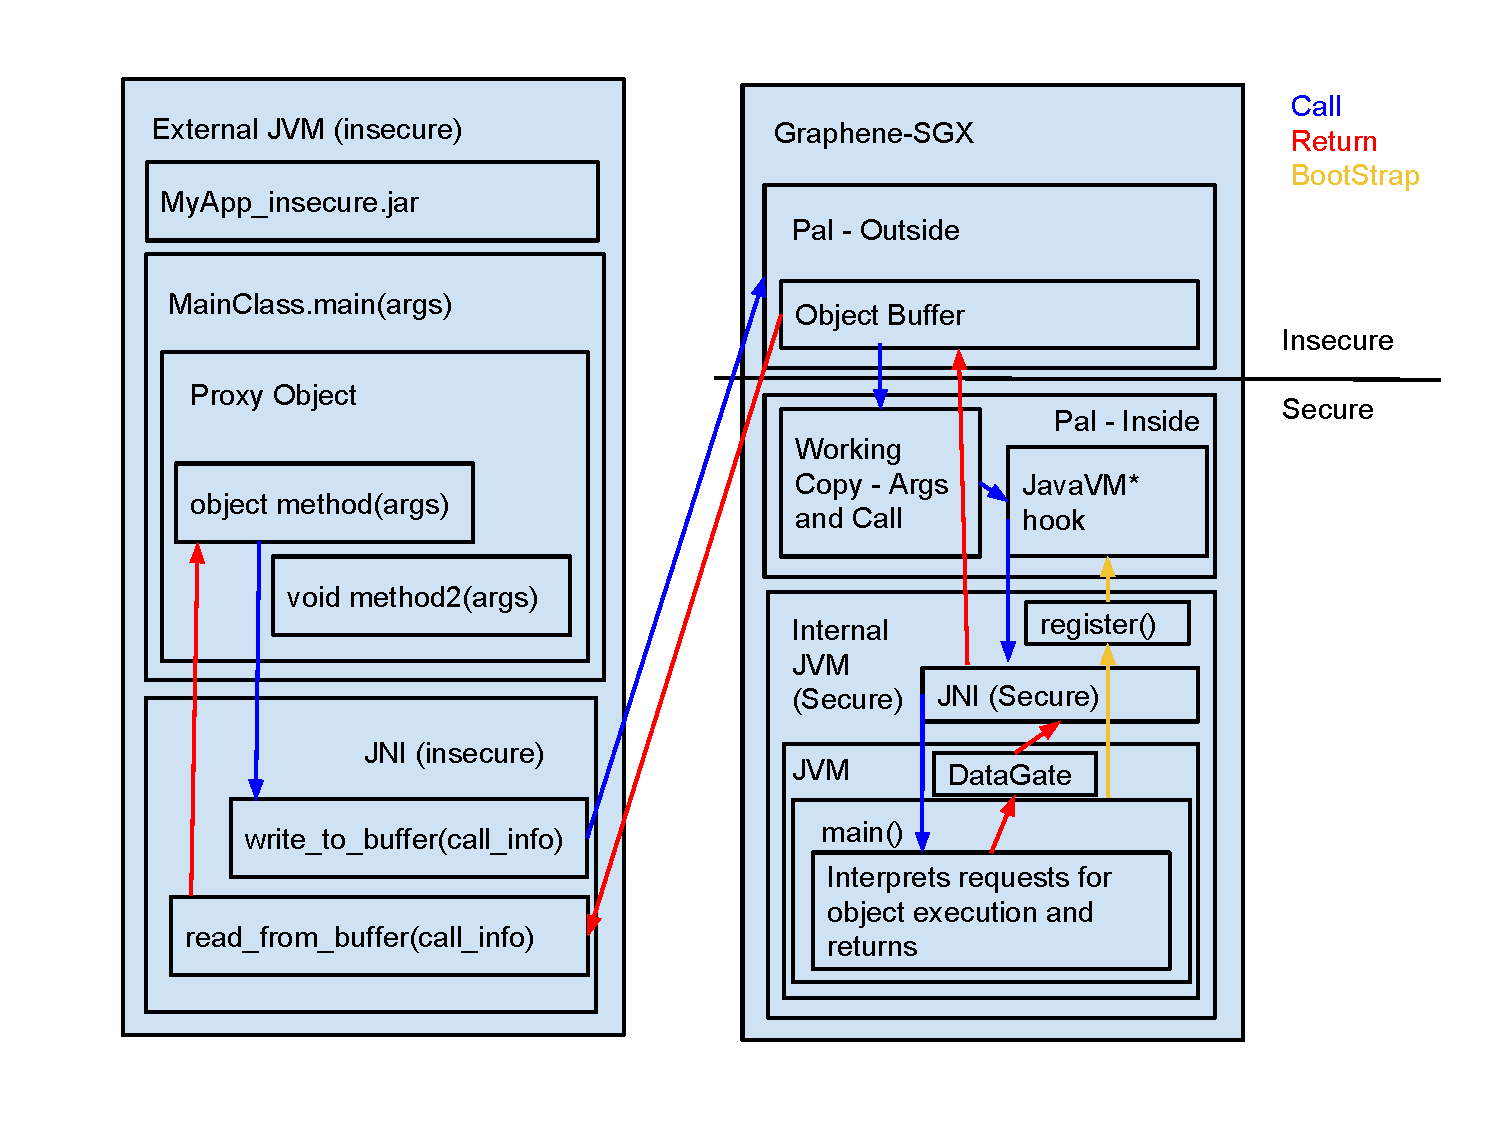
\includegraphics[width=\linewidth]{civet_flow.pdf}}
%\caption{Cevit Architecture and control flow.}
%\label{fig:architecture}
%\end{figure}

%\sysname{} leverages JAVA, a managed language 
%runtime, to help thwart the attacks discussed in 
%section~\ref{sec:background}. The modularity of JAVA 
%allows automatic partitioning of applications to 
%reduce the number of classes added to the Trusted 
%Computing Base. The type-safety property enforced by 
%JAVA runtime avoids exploitation of memory-safety 
%vulnerabilities in the application . JAVA framework 
%also eases the information flow tracking to prevent 
%information leakage due to buggy code. Moreover, 
%\sysname{} uses JAVA runtime to seamlessly 
%provision secure objects and classes in the enclave.




%\subsection{Automatic Partitioning of JAVA Applications}
%\subsection{Preventing Information Leakage}
%\subsection{Seamless Provisioning of Secure Objects and Classes}

\section{Implementation Details}
\label{sec:implementation}

In this section, we discuss in detail about how the framework of \sysname{}
is implemented. 

\paragraph{The \graphene{} \libos{} ported to \sgx{}}
Similar to Drawbridge~\cite{porter11drawbridge}
in Haven~\cite{baumann14haven},
\graphene{}~\cite{tsai14graphene} maps a larger number of Linux system APIs
to a narrow, portable host interface.
Library OSes like Drawbridge and Haven unlock the platform limitations of \sgx{} and
allows many applications to be ported to enclave painlessly.
%The untrusted interface of \graphene{} \libos{} after porting to \sgx{}
%is mostly identical to the original host interface,
%therefore \graphene{} has a finite  bound on interface for the enclave.

%\graphene{} uses checksums to verify the integrity of applications.
%The checksums are collected by a compile-time Signer tool of \graphene{}.
%The Signer tool ensures the integrity of the file checksums
%by including them as part of the enclave's measurement.
%Even if the same \libos{} is used
%to run the applications,
%different binaries in the enclaves yield different measurements. 
%Such a design decouples the problem of distributing 
%and guaranteeing code integrity for each application, as the enclave integrity is based on the integrity of the application --- not just the libOS.
 
\sysname{} makes minor modifications to \graphene{} to allow
the enclave to run
in the same process as the the untrusted \jvm{}.
The trusted and untrusted VM share a ring buffer (as shown in Figure~\ref{fig:runtime} for communication during control transfer,
but the ring buffer itself is not trusted. The \sysname{} framework encrypts tainted security-sensitive data before passing the data on the ring buffer.
 
\paragraph{Control transfer at enclave entry}

\sysname{} transparently transfers the control from the untrusted classes to trusted classes --- triggering enclave entry in the process ---
by intercepting the trusted classes's method or constructor invocation by untrusted classes.
\sysname{} intercepts classes in two ways:
(a) For an entry class that has finite entry points,
\sysname{} creates a wrapper class that redirects all constructors and static methods.
(b) For other trusted classes, \sysname{} adds the redirection calls only when a reference is returned by the enclave. %\fixmebj{Is this correct?}
%(b) For other trusted classes, the interception is installed when a reference of 
%object is returned to the untrusted classes.
On future access of the object in the enclave, a proxy object is created to trigger the interception, using CGLib.

When the control transfers between the trusted and untrusted classes,
the arguments and return values of the methods
are stored in the ring buffer.
\sysname{} relies on serialization and deserialization to safely transfer object in and out of the enclave.
When \sysname{} deserializes an object, the \jvm{} perform type-checking sanitize the input. % the members.

%After \sysname{} transfers the arguments, the \jvm{} thread that
%invoke the intercepted  method does not directly enter the enclave.
%On the other hand, several enclave threads that are pre-created during the enclave creation that are block-waiting on the ring buffer.
%One of the enclave threads consumes the queued job, invokes the method,
%and returns to block-waiting for more new requests.
%No variable on the stack has to be persistent for the enclave threads,
%and only instances of the trusted classes are persisted across enclave entry and exit.

%Moreover, upon enclave entry and exit, the objects that can be safely transferred in or out of the enclave must be serialized / deserialized.
%However, not all classes implement the interface {\tt Serializable},
%especially when the classes contain internal states that cannot be simply interpreted.
%But, \sysname{} assumes that the types of all arguments and return objects must be {\tt Serializable}. 

\paragraph{Limitations}
As we leverage dependency tracking for automated partition, there are few corner cases that the Shredder cannot gracefully handle.
Because CGLib creates subclasses of objects when intercepting them,
it requires the intercepted object to be never finalized.
If a trusted class is also a final class, developers have to manually modify the class definition. Even though final attribute prevents further extension of the class, we argue that the application developer who is building the enclave can safely remove the final attribute as the \sysname{} signs the enclave jar.

 We also do not let trusted classes make method or constructor invocation of the untrusted classes, as the untrusted classes may be able to influence and interfere with the execution of trusted classes. Moreover, we only consider the provisioned code and data as security-sensitive. Even though this limits the usage scenarios, we argue that for any right usage of \sgx{} hardware, these limitations are not disruptive.

%\input{Implementation Details}
%% ASPLOS
%\input{cloud}
%\input{Case Studies}
\section{Case Studies}
\label{sec:case-study}

In order to evaluate the utility of \sysname{}, we partitioned
several example \java{} applications, which we use in our evaluation.


\paragraph{Session Encryption in SSH Client/Server.}
%Code that handles security sensitive data
In order to show the ability of \sysname{} to protect a 
confidential data and avoid leaking that data,
%A \java{} program with a secret that is either generated during runtime
%or provisioned from trusted remote enclaves,
%can be partitioned and secured by \sysname{} to prevent leaking the secret.
%We demonstrate this use case
%using 
we partitioned a \java{}-based SSH client and server~\citep{apache-sshd}.
In this case, the protected secret is the session key.
%For an SSH connection, one primary secret that needs to be secured
%is the session key used for encrypting and decrypting the data
%between the two communicating parties.
For both the SSH client and server, we create
a control class in the enclave that includes 
the key generator, encryption engine objects, secret key
and the {\em BouncyCastle}~\citep{bouncycastle} cryptography library.
The rest of the application is outside of the enclave.
%from the rest of the application.
%\fixmedp{surprising the private key isn't also in the enclave}

We use information flow tracking to ensure that the only data
leaving the enclave is ciphertext output from the encryption algorithm,
or plaintext returned from the decryption algorithm.
This involves adding lines to the end of both algorithms, and does assume that
the encryption and decryption functions are implemented correctly.
Attempts to copy the session key directly into an output buffer at any other point in the code
will result in encryption of the buffer before leaving the enclave.

{\tt org.apache.sshd.common.FactoryManager} is identified as the entry class for Shredder, because this class returns all the objects required for the SSH Protocol.
Shredder generates the enclave image that includes the secret key classes, random generator, key generator, engine for diffie-hellman key-exchange, and encryption-decryption engine. Both the client as well as the server are partitioned to be run using \sysname{}. The client and server first mutually attests each other, exchange the key, and then setup the secure session. We use these SSH client and server for transferring files using SFTP. For simplicity, we run both client and the server on the same host, but in different enclaves. 
%We measure the bandwidth of file transfer as discussed in \S\ref{sec:eval:perf}

%\fixmedp{I took some liberty here: We have to be able to receive data too, right?  Also, I would be more careful with the use of ``guarantee'' in general}

%% The information flow filtering guarantees that no part of the session key
%% can leak from the enclave despite any vulnerabilities 
%% in the crypto library or the control class.
%% The only data that can be released from the enclave
%% is the cipher text of the inputs from the SSH client and server,
%% encrypted with the session key, after declassification.
%% We only had to add only one line of code to declassify the cipher text using the {\tt Enclave.declassify(ciphertext)} API. Thus, in addition to only identifying classes with sensitive information, the developers have to just add one statement per declassifying location in the enclave classes.

\paragraph{Secret Hadoop Algorithm.}
%Code that contains a secret algorithm
\sysname{} not only protects confidential data, but also protects confidential code.
For instance, if a company has developed an analysis tool that gives them a essential competitive advantage,
they must either run their own data center or trust a cloud provider not to leak their tool 
to any competitors.
%, such 
%as trade secret, that developers intend to protect from insecure system stack.

To demonstrate this use case, we modify a Hadoop sort algorithm~\citep{hadoop-sort},
so that the implementation of its Partitioner, Mapper, Combiner, Sorter and Reducer
are isolated from the rest of the Hadoop infrastructure. 
The algorithm sorts values from a key-value store, in which
the input keys and values are encrypted.
The output of the sorting algorithm is a sorted, encrypted key value store.
%based on original values a key-value store, in which
%both input keys and values are encrypted.

The Hadoop framework schedules proxy Partitioners, Mappers, Combiners, Sorters, and Reducers,
and then creates enclaves for these classes.
Once a baseline \sysname{} enclave is created, encrypted class files
are downloaded from a trusted server using our remote attestation tools,
and then decrypted, loaded, and measured for integrity. 
%We evaluate the Job completion time for our sort algorithm in \S\ref{sec:eval:perf}.
%, requests for the real classes to be provisioned from a trusted server, loads, and executes the provisioned classes.

The information flow control at the enclave border protects against
accidental output of a plaintext key-value pair from the encrypted store,
as well as protects the class code file itself.
Similarly, intermediate state from the code cannot be inadvertently returned by a function to the untrusted Hadoop framework,
although we do allow encrypted outputs to be passed from a Mapper to a Combiner or Reducer.
The contents of any code cannot be leaked outside enclave by copying the code into an output object, as the tainted object is automatically encrypted before leaving enclave. %\fixmedp{does this just happen naturally?},
Also, in conjunction with the trusted remote server, we rate-limit instantiations of the code to mitigate the risk of
brute-force mapping of its outputs or reverse-engineering the code.


%% any output of the isolated classes ---
%% even if it is just an intermediate state ---
%% is encrypted before leaving the enclave.
%% \sysname{} not only protects the implementation of the algorithm,
%% but any output of the algorithm that may potentially help attackers
%% reverse-engineer the implementation. The {\em confidential code} property of ~\sysname{} is not limited to Hadoop, but can also be leveraged by standard \java{} applications.

\paragraph{Secure Data Manager Web-app.}
%JAVA Web-start Application
\sysname{} can also secure {\em Java Network Launch Protocol} (JNLP) applets and web-start apps, effectively 
extending trust from a remote trusted server to a client enclave using any web-app 
plugged into a supported browser. This allows the developers to offload some of the 
computation on secret data to the client machine from the trusted server.
%\java{} applications in the form of
%can also be secured by \sysname{}. 

For instance, in a large medical hospital with a centralized repository of patient data,
the doctors may want to access any patient data from any terminal using a web browser.
A web developer can design an applet such as Secure Data 
Manager(SDM)~\citep{sdm-applet} to store the secret patient data on a client machine, 
and display this information securely using Intel Protected Audio and Video Path 
(PAVP) technology~\citep{intel-pavp}.
However, to protect the sensitive patient information from untrusted system stack, the 
developer can use \sysname{} to isolate the classes that represent the secure data 
in an enclave. The developer just has to identify such classes representing the secret 
data and display methods, and the \sysname{} seamlessly creates enclave for 
managing secret data.
% or perform computations on secret data isolated in an enclave.
%We demonstrate this use case using a 
%\fixmedp{what is the practial use case?  Like, what is the data actually used for?}
The trusted data manager class authenticates the doctor and loads the provisioned data 
from the remote trusted server. The Intel PAVP enabled displays can then take the input from the display methods of the trusted data manager class.

For simplicity, we only partition and run the SDM applet from a browser without the support for Intel PAVP display devices. We identify four classes --- {\tt SafetyBox}, 
{\tt AuthenticationInfo}, {\tt LoginEntry}, and {\tt Type} --- as entry class to the Shredder and generate a web-start app image containing the enclave image. The web-app loads normally, and when it tries to access any of the above four classes, \sysname{} seamlessly creates an enclave for those objects. 
%We measure the latency of I/O from the SDM in \S\ref{sec:eval:perf}.


%\fixmedp{This last example is pretty content free.  Can you give me an example of a web app that would use this, and flesh out the story a bit?}

\chapter{Evaluation}
\label{chap:eval}
%\subsection{Other Related Works}

\section{Summary}
\label{sec:graphene:summary}

The \graphene{} design is centered around
building a para-virtualized layer, which can reuse the OS components for reproducing Linux system interfaces.
%instead of building arbitrary compatibility layers for reproducing the system interface.
%constantly porting the significant  of the existing system interface.
%In \graphene{}, 
\graphene{} defines a host ABI, as a new boundary between the OS and user space.
The host ABI is simple enough to port (containing \palcalls{} functions),
and exports sufficient functionality for virtualizing a primary part of the system API components.
A library OS is built upon the host ABI,
and implements \graphenesyscalls{} Linux system calls to reuse unmodified Linux applications.
\graphene{} decouples the development for a compatibility layer,
from host-specific challenges to building OS features, and isolating applications from other malicious tenants.



%\sysname{} extends library OS designs 
%to include multi-process APIs required by common applications, such as a shell or 
%web server.
%\sysname{} demonstrates efficient, selective
%coordination of shared state across multiple library OS 
%instances---maintaining host independence.
%%simplifying security sandboxing of otherwise unwieldy OS features.
%Applications on \sysname{} enjoy both 
%strong security isolation with acceptable performance and low memory overheads.
%% from unrelated programs 
%%and seamless shared namespaces 
%%among a group of coordinating guests.
%%% Although this paper focuses on distributed coordination
%%% to facilitate the efficiency benefits,
%%% expect our experiences with distributed coordination 
%%% may also be particularly relevant to highly scalable OS designs, 
%%% which avoid the bottlenecks of shared OS data structures~\cite{baumann09barrelfish, song11eurosys}.
%%Graphene's overheads are acceptable and the memory 
%%footprint is substantially lower than a VM.



%% , which could benefit from the reduced memory footprint
%% in a cloud 

%% by introducing a novel design for  coordination APIs. 
%% to a new OS (Linux),
%% new classes of applications,
%% and introduces a
%% %an alternative design point for storage virtualization.
%% Our results further demonstrate the feasibility of the library OS model.
%% % generally,
%% Applications on Graphene enjoy both 
%% strong security isolation from unrelated programs 
%% and seamless shared namespaces 
%% among a group of coordinating guests.
%% Although we explore this concept in a library OS,
%% we expect the namespace coordination framework 
%% could also be adapted to limit the attack surface area between
%% processes in a traditional OS.
%% We expect these experiences with distributed coordination 
%% may also be particularly relevant to highly scalable OS designs, 
%% which avoid the bottlenecks of shared OS data structures~\cite{baumann09barrelfish}.
%and specifically of content-addressable storage as the primary virtual storage abstraction.
%%% This work opens up a number of interesting questions for future work, 
%%% including studying opportunities for low-level storage optimization within the CAS server,
%%% making CAS the root file system,
%%% eliminating storage management in the host kernel, and 
%%% investigating the impact of frequent migration among devices.

\begin{comment}
Enabling legacy applications in a restricted environment,
such as \picoprocs{} or enclaves,
requires extra effort for mitigating the limitations of platforms,
in order to support typical OS personalities.
\graphene{}, as described in this chapter, extends the existing \libos{} designs
from isolating single-process or unshared abstractions
to include multi-process APIs required by many UNIX applications,
such as servers or shell scripts.
The challenge that \graphene{} primarily overcomes
is the requirement for coordinating shared states across multiple \picoprocs{},
to provides a collaborative, unified OS view.
Essentially, \graphene{} implements all shared, multi-process abstractions
and OS states
based on coordination over host-provided, pipe-like RPC streams.
The RPC-based, distributed OS implementation enables multi-process support in \graphene{}, with minimal extension to the host interface,
and a sweet-spot for enforcing inter-application security isolation,
by simply sandboxing the RPC streams.
Such a model largely reduces the complexity of
enforcing security isolation
on idiosyncratic multi-process abstractions
and shared states.
Because the corporative nature of \picoprocs{} in \graphene{},
an application can even dynamically impose sandboxing on one of its processes,
to reflect per-process, variable security policies.
\end{comment}

\begin{comment}
In principle, we attempt to use \graphene{} to justify the platform independence
of the \libos{} design,
without sacrificing its qualitative benefits,
such as isolating mutually-untrusting applications
and a narrow attack surface to kernels.
\graphene{} implements a considerable number of common Linux system calls,
to support popular, modern applications
such as Apache web server, GNU Make, OpenJDK \java{} VM and the Python runtime.
\graphene{} translates the high-level system APIs used by applications
to a host ABI
inherited and extended from a previous Windows-compatible \libos{}~\cite{porter11drawbridge}.
In addition, we port the \pal{} (Platform Adaption Layer) of \graphene{}
to various platforms,
including FreeBSD, OSX, Windows, and even a more restricted environment, the \intel{} \sgx{} enclaves.
In particular, \graphene{} being ported to \intel{} \sgx{}
(\graphenesgx{})
can isolate applications --- either single-process or multi-process
--- on a host where neither the operating system nor the hardware (except the CPU package)
is trusted by the applications. 
Overall, \graphene{} shows that,
by simply porting the reasonably sized host ABI
to a new platform,
a whole large spectrum of legacy applications tested on the previous platforms
can be activated all together.
\end{comment}


\makeatletter
\def\input@path{{}}
\makeatother
\graphicspath{{}}
